\documentclass[twoside]{book}

% Packages required by doxygen
\usepackage{calc}
\usepackage{doxygen}
\usepackage{graphicx}
\usepackage[utf8]{inputenc}
\usepackage{makeidx}
\usepackage{multicol}
\usepackage{multirow}
\usepackage{textcomp}
\usepackage[table]{xcolor}

% Font selection
\usepackage[T1]{fontenc}
\usepackage{mathptmx}
\usepackage[scaled=.90]{helvet}
\usepackage{courier}
\usepackage{amssymb}
\usepackage{sectsty}
\renewcommand{\familydefault}{\sfdefault}
\allsectionsfont{%
  \fontseries{bc}\selectfont%
  \color{darkgray}%
}
\renewcommand{\DoxyLabelFont}{%
  \fontseries{bc}\selectfont%
  \color{darkgray}%
}

% Page & text layout
\usepackage{geometry}
\geometry{%
  a4paper,%
  top=2.5cm,%
  bottom=2.5cm,%
  left=2.5cm,%
  right=2.5cm%
}
\tolerance=750
\hfuzz=15pt
\hbadness=750
\setlength{\emergencystretch}{15pt}
\setlength{\parindent}{0cm}
\setlength{\parskip}{0.2cm}
\makeatletter
\renewcommand{\paragraph}{%
  \@startsection{paragraph}{4}{0ex}{-1.0ex}{1.0ex}{%
    \normalfont\normalsize\bfseries\SS@parafont%
  }%
}
\renewcommand{\subparagraph}{%
  \@startsection{subparagraph}{5}{0ex}{-1.0ex}{1.0ex}{%
    \normalfont\normalsize\bfseries\SS@subparafont%
  }%
}
\makeatother

% Headers & footers
\usepackage{fancyhdr}
\pagestyle{fancyplain}
\fancyhead[LE]{\fancyplain{}{\bfseries\thepage}}
\fancyhead[CE]{\fancyplain{}{}}
\fancyhead[RE]{\fancyplain{}{\bfseries\leftmark}}
\fancyhead[LO]{\fancyplain{}{\bfseries\rightmark}}
\fancyhead[CO]{\fancyplain{}{}}
\fancyhead[RO]{\fancyplain{}{\bfseries\thepage}}
\fancyfoot[LE]{\fancyplain{}{}}
\fancyfoot[CE]{\fancyplain{}{}}
\fancyfoot[RE]{\fancyplain{}{\bfseries\scriptsize Generated on Fri Jan 30 2015 13\-:05\-:35 for R\-P\-V-\/\-L\-F\-V-\/\-Analyzer by Doxygen }}
\fancyfoot[LO]{\fancyplain{}{\bfseries\scriptsize Generated on Fri Jan 30 2015 13\-:05\-:35 for R\-P\-V-\/\-L\-F\-V-\/\-Analyzer by Doxygen }}
\fancyfoot[CO]{\fancyplain{}{}}
\fancyfoot[RO]{\fancyplain{}{}}
\renewcommand{\footrulewidth}{0.4pt}
\renewcommand{\chaptermark}[1]{%
  \markboth{#1}{}%
}
\renewcommand{\sectionmark}[1]{%
  \markright{\thesection\ #1}%
}

% Indices & bibliography
\usepackage{natbib}
\usepackage[titles]{tocloft}
\setcounter{tocdepth}{3}
\setcounter{secnumdepth}{5}
\makeindex

% Hyperlinks (required, but should be loaded last)
\usepackage{ifpdf}
\ifpdf
  \usepackage[pdftex,pagebackref=true]{hyperref}
\else
  \usepackage[ps2pdf,pagebackref=true]{hyperref}
\fi
\hypersetup{%
  colorlinks=true,%
  linkcolor=blue,%
  citecolor=blue,%
  unicode%
}

% Custom commands
\newcommand{\clearemptydoublepage}{%
  \newpage{\pagestyle{empty}\cleardoublepage}%
}


%===== C O N T E N T S =====

\begin{document}

% Titlepage & ToC
\pagenumbering{roman}
\begin{titlepage}
\vspace*{7cm}
\begin{center}%
{\Large R\-P\-V-\/\-L\-F\-V-\/\-Analyzer }\\
\vspace*{1cm}
{\large Generated by Doxygen 1.8.5}\\
\vspace*{0.5cm}
{\small Fri Jan 30 2015 13:05:35}\\
\end{center}
\end{titlepage}
\clearemptydoublepage
\tableofcontents
\clearemptydoublepage
\pagenumbering{arabic}

%--- Begin generated contents ---
\chapter{githookcontroller}
\label{md_hooks_README}
This repository contains the githookcontroller, a general tool to construct git hooks for git\-Hub based projects without a central contral server.

\subsection*{Using githookcontroller in your repo\-:}

\subsubsection*{Setup\-:}

The easiest way to implement the githookcontroller to your repo is to add setup script as shown in the setup.\-sh.\-example file and run it from the root directory of your repo. \subsubsection*{Adjusting the hooks}

Githookcontroller ships with some exampe hook implementations, which you may want to adjust. The standard way to use the githookcontroller is to create a Git\-Hook\-Controller class object within a python hook script, parse hook infos if necessary and call member functions of the controller (e.\-g. update doxygen) to perform hook actions as needed.

\subsubsection*{Currently implemented features\-:}


\begin{DoxyItemize}
\item Parse output from pre-\/commit hooks.
\item Parse which files are changed in a commit.
\item Several easy to use controller class properties\-: current\-\_\-branch, tracked remote\-\_\-branches, local and remote root directory name, remote url.
\item Function to checkout different branches in local repo.
\item Create branch specific doxygen documentation on every commit (see hooks/pre-\/commit). Doxygen documentation without warnig can be enfoced based on repo root and branch name.
\item Add doxygen documentation for given branches to gh-\/pages branch (see hooks/pre-\/push). 
\end{DoxyItemize}
\chapter{Namespace Index}
\section{Namespace List}
Here is a list of all namespaces with brief descriptions\-:\begin{DoxyCompactList}
\item\contentsline{section}{\hyperlink{namespacegithookcontroller}{githookcontroller} }{\pageref{namespacegithookcontroller}}{}
\item\contentsline{section}{\hyperlink{namespacepost-commit}{post-\/commit} }{\pageref{namespacepost-commit}}{}
\item\contentsline{section}{\hyperlink{namespacepre-commit}{pre-\/commit} }{\pageref{namespacepre-commit}}{}
\item\contentsline{section}{\hyperlink{namespacepre-push}{pre-\/push} }{\pageref{namespacepre-push}}{}
\end{DoxyCompactList}

\chapter{Hierarchical Index}
\section{Class Hierarchy}
This inheritance list is sorted roughly, but not completely, alphabetically\-:\begin{DoxyCompactList}
\item Analysis\-Process\begin{DoxyCompactList}
\item \contentsline{section}{special\-Ana}{\pageref{classspecialAna}}{}
\end{DoxyCompactList}
\item \contentsline{section}{Cuts}{\pageref{classCuts}}{}
\item \contentsline{section}{githookcontroller.\-Git\-Hook\-Controller}{\pageref{classgithookcontroller_1_1GitHookController}}{}
\end{DoxyCompactList}

\chapter{Class Index}
\section{Class List}
Here are the classes, structs, unions and interfaces with brief descriptions\-:\begin{DoxyCompactList}
\item\contentsline{section}{\hyperlink{classCuts}{Cuts} }{\pageref{classCuts}}{}
\item\contentsline{section}{\hyperlink{classgithookcontroller_1_1GitHookController}{githookcontroller.\-Git\-Hook\-Controller} }{\pageref{classgithookcontroller_1_1GitHookController}}{}
\item\contentsline{section}{\hyperlink{classspecialAna}{special\-Ana} }{\pageref{classspecialAna}}{}
\end{DoxyCompactList}

\chapter{File Index}
\section{File List}
Here is a list of all files with brief descriptions\-:\begin{DoxyCompactList}
\item\contentsline{section}{\hyperlink{CutClass_8hh}{Cut\-Class.\-hh} }{\pageref{CutClass_8hh}}{}
\item\contentsline{section}{\hyperlink{specialAna_8cc}{special\-Ana.\-cc} }{\pageref{specialAna_8cc}}{}
\item\contentsline{section}{\hyperlink{specialAna_8hh}{special\-Ana.\-hh} }{\pageref{specialAna_8hh}}{}
\item\contentsline{section}{hooks/\hyperlink{githookcontroller_8py}{githookcontroller.\-py} }{\pageref{githookcontroller_8py}}{}
\item\contentsline{section}{hooks/\hyperlink{post-commit_8py}{post-\/commit.\-py} }{\pageref{post-commit_8py}}{}
\item\contentsline{section}{hooks/\hyperlink{pre-commit_8py}{pre-\/commit.\-py} }{\pageref{pre-commit_8py}}{}
\item\contentsline{section}{hooks/\hyperlink{pre-push_8py}{pre-\/push.\-py} }{\pageref{pre-push_8py}}{}
\end{DoxyCompactList}

\chapter{Namespace Documentation}
\section{githookcontroller Namespace Reference}
\label{namespacegithookcontroller}\index{githookcontroller@{githookcontroller}}
\subsection*{Classes}
\begin{DoxyCompactItemize}
\item 
class \hyperlink{classgithookcontroller_1_1GitHookController}{Git\-Hook\-Controller}
\end{DoxyCompactItemize}
\subsection*{Functions}
\begin{DoxyCompactItemize}
\item 
def \hyperlink{namespacegithookcontroller_a5c0a2facfdd7509f64df2aa6aefecf17}{main}
\end{DoxyCompactItemize}
\subsection*{Variables}
\begin{DoxyCompactItemize}
\item 
tuple \hyperlink{namespacegithookcontroller_a3bbdf7a562461bd3baca4ef635d6dd50}{log} = logging.\-get\-Logger( 'githookcontroller' )
\item 
tuple \hyperlink{namespacegithookcontroller_a13f0aa9843a2a5b05ba2e12f5ed3c903}{ch} = logging.\-Stream\-Handler( sys.\-stdout )
\item 
tuple \hyperlink{namespacegithookcontroller_a8672f684f117c8c4733546a0bc9e9616}{formatter} = logging.\-Formatter( '\%(levelname)s (\%(name)s)\-: \%(message)s' )
\item 
tuple \hyperlink{namespacegithookcontroller_ae617d8e0c886ed4e082bd11f1f33bd0d}{Push}
\item 
tuple \hyperlink{namespacegithookcontroller_af0d83e4b5f26b63a7ee452f3eb566ef4}{Commit}
\end{DoxyCompactItemize}


\subsection{Function Documentation}
\index{githookcontroller@{githookcontroller}!main@{main}}
\index{main@{main}!githookcontroller@{githookcontroller}}
\subsubsection[{main}]{\setlength{\rightskip}{0pt plus 5cm}def githookcontroller.\-main (
\begin{DoxyParamCaption}
{}
\end{DoxyParamCaption}
)}\label{namespacegithookcontroller_a5c0a2facfdd7509f64df2aa6aefecf17}


Definition at line 450 of file githookcontroller.\-py.



\subsection{Variable Documentation}
\index{githookcontroller@{githookcontroller}!ch@{ch}}
\index{ch@{ch}!githookcontroller@{githookcontroller}}
\subsubsection[{ch}]{\setlength{\rightskip}{0pt plus 5cm}tuple githookcontroller.\-ch = logging.\-Stream\-Handler( sys.\-stdout )}\label{namespacegithookcontroller_a13f0aa9843a2a5b05ba2e12f5ed3c903}


Definition at line 37 of file githookcontroller.\-py.

\index{githookcontroller@{githookcontroller}!Commit@{Commit}}
\index{Commit@{Commit}!githookcontroller@{githookcontroller}}
\subsubsection[{Commit}]{\setlength{\rightskip}{0pt plus 5cm}tuple githookcontroller.\-Commit}\label{namespacegithookcontroller_af0d83e4b5f26b63a7ee452f3eb566ef4}
{\bfseries Initial value\-:}
\begin{DoxyCode}
1 = namedtuple(\textcolor{stringliteral}{'Commit'}, [\textcolor{stringliteral}{'local\_ref'}, \textcolor{stringliteral}{'local\_sha1'}, \textcolor{stringliteral}{'remote\_ref'}, \textcolor{stringliteral}{'remote\_sha1'},
2                                \textcolor{stringliteral}{'local\_branch'}, \textcolor{stringliteral}{'remote\_branch'}])
\end{DoxyCode}


Definition at line 45 of file githookcontroller.\-py.



Referenced by githookcontroller.\-Git\-Hook\-Controller.\-parse\-\_\-pre\-\_\-push().

\index{githookcontroller@{githookcontroller}!formatter@{formatter}}
\index{formatter@{formatter}!githookcontroller@{githookcontroller}}
\subsubsection[{formatter}]{\setlength{\rightskip}{0pt plus 5cm}tuple githookcontroller.\-formatter = logging.\-Formatter( '\%(levelname)s (\%(name)s)\-: \%(message)s' )}\label{namespacegithookcontroller_a8672f684f117c8c4733546a0bc9e9616}


Definition at line 39 of file githookcontroller.\-py.

\index{githookcontroller@{githookcontroller}!log@{log}}
\index{log@{log}!githookcontroller@{githookcontroller}}
\subsubsection[{log}]{\setlength{\rightskip}{0pt plus 5cm}tuple githookcontroller.\-log = logging.\-get\-Logger( 'githookcontroller' )}\label{namespacegithookcontroller_a3bbdf7a562461bd3baca4ef635d6dd50}


Definition at line 35 of file githookcontroller.\-py.

\index{githookcontroller@{githookcontroller}!Push@{Push}}
\index{Push@{Push}!githookcontroller@{githookcontroller}}
\subsubsection[{Push}]{\setlength{\rightskip}{0pt plus 5cm}tuple githookcontroller.\-Push}\label{namespacegithookcontroller_ae617d8e0c886ed4e082bd11f1f33bd0d}
{\bfseries Initial value\-:}
\begin{DoxyCode}
1 = namedtuple(\textcolor{stringliteral}{'Push'}, [\textcolor{stringliteral}{'commits'}, \textcolor{stringliteral}{'remote\_name'}, \textcolor{stringliteral}{'remote\_url'},
2                            \textcolor{stringliteral}{'current\_branch'}, \textcolor{stringliteral}{'removing\_remote'}, \textcolor{stringliteral}{'forcing'}])
\end{DoxyCode}


Definition at line 43 of file githookcontroller.\-py.



Referenced by githookcontroller.\-Git\-Hook\-Controller.\-parse\-\_\-pre\-\_\-push().


\section{post-\/commit Namespace Reference}
\label{namespacepost-commit}\index{post-\/commit@{post-\/commit}}

\section{pre-\/commit Namespace Reference}
\label{namespacepre-commit}\index{pre-\/commit@{pre-\/commit}}
\subsection*{Variables}
\begin{DoxyCompactItemize}
\item 
tuple \hyperlink{namespacepre-commit_a95f05a041aa51857ded4a498e766b83d}{git\-Controller} = \hyperlink{classgithookcontroller_1_1GitHookController}{Git\-Hook\-Controller}()
\item 
tuple \hyperlink{namespacepre-commit_a1c824fbe54d00a54423cb4955f97dcf5}{changed} = git\-Controller.\-parse\-\_\-pre\-\_\-commit()
\end{DoxyCompactItemize}


\subsection{Variable Documentation}
\index{pre-\/commit@{pre-\/commit}!changed@{changed}}
\index{changed@{changed}!pre-commit@{pre-\/commit}}
\subsubsection[{changed}]{\setlength{\rightskip}{0pt plus 5cm}tuple pre-\/commit.\-changed = git\-Controller.\-parse\-\_\-pre\-\_\-commit()}\label{namespacepre-commit_a1c824fbe54d00a54423cb4955f97dcf5}


Definition at line 11 of file pre-\/commit.\-py.

\index{pre-\/commit@{pre-\/commit}!git\-Controller@{git\-Controller}}
\index{git\-Controller@{git\-Controller}!pre-commit@{pre-\/commit}}
\subsubsection[{git\-Controller}]{\setlength{\rightskip}{0pt plus 5cm}tuple pre-\/commit.\-git\-Controller = {\bf Git\-Hook\-Controller}()}\label{namespacepre-commit_a95f05a041aa51857ded4a498e766b83d}


Definition at line 9 of file pre-\/commit.\-py.


\section{pre-\/push Namespace Reference}
\label{namespacepre-push}\index{pre-\/push@{pre-\/push}}
\subsection*{Variables}
\begin{DoxyCompactItemize}
\item 
tuple \hyperlink{namespacepre-push_a8c127aba641727d65b14a0f4aad44a1c}{git\-Controller} = \hyperlink{classgithookcontroller_1_1GitHookController}{Git\-Hook\-Controller}()
\item 
tuple \hyperlink{namespacepre-push_a71bb0fe33ffeefadee67d3dbbe085080}{push} = git\-Controller.\-parse\-\_\-pre\-\_\-push()
\item 
list \hyperlink{namespacepre-push_a78ac8288356df9910db91d02884f211c}{branchnames} = \mbox{[}commit.\-local\-\_\-branch for commit in push.\-commits\mbox{]}
\end{DoxyCompactItemize}


\subsection{Variable Documentation}
\index{pre-\/push@{pre-\/push}!branchnames@{branchnames}}
\index{branchnames@{branchnames}!pre-push@{pre-\/push}}
\subsubsection[{branchnames}]{\setlength{\rightskip}{0pt plus 5cm}list pre-\/push.\-branchnames = \mbox{[}commit.\-local\-\_\-branch for commit in push.\-commits\mbox{]}}\label{namespacepre-push_a78ac8288356df9910db91d02884f211c}


Definition at line 34 of file pre-\/push.\-py.

\index{pre-\/push@{pre-\/push}!git\-Controller@{git\-Controller}}
\index{git\-Controller@{git\-Controller}!pre-push@{pre-\/push}}
\subsubsection[{git\-Controller}]{\setlength{\rightskip}{0pt plus 5cm}tuple pre-\/push.\-git\-Controller = {\bf Git\-Hook\-Controller}()}\label{namespacepre-push_a8c127aba641727d65b14a0f4aad44a1c}


Definition at line 30 of file pre-\/push.\-py.

\index{pre-\/push@{pre-\/push}!push@{push}}
\index{push@{push}!pre-push@{pre-\/push}}
\subsubsection[{push}]{\setlength{\rightskip}{0pt plus 5cm}tuple pre-\/push.\-push = git\-Controller.\-parse\-\_\-pre\-\_\-push()}\label{namespacepre-push_a71bb0fe33ffeefadee67d3dbbe085080}


Definition at line 33 of file pre-\/push.\-py.


\chapter{Class Documentation}
\section{Cuts Class Reference}
\label{classCuts}\index{Cuts@{Cuts}}


{\ttfamily \#include $<$Cut\-Class.\-hh$>$}

\subsection*{Public Member Functions}
\begin{DoxyCompactItemize}
\item 
\hyperlink{classCuts_a8c24c150ccef259ae6ebc3051dc32658}{Cuts} ()
\item 
\hyperlink{classCuts_a7b563df83f6e6bfabc4d605d5a809aca}{Cuts} (const std\-::string name)
\item 
\hyperlink{classCuts_a8d012671d52feca2353658e81bb5055c}{Cuts} (const std\-::string name, int i\-\_\-n\-\_\-bins\-\_\-x, double i\-\_\-x\-\_\-min, double i\-\_\-x\-\_\-max)
\item 
\hyperlink{classCuts_afc57873c550bee21a77e747d0c647f44}{Cuts} (const std\-::string name, int i\-\_\-n\-\_\-bins\-\_\-x, double i\-\_\-x\-\_\-min, double i\-\_\-x\-\_\-max, std\-::string i\-\_\-x\-\_\-title)
\item 
\hyperlink{classCuts_adc1fca90f6426f31e3100e4ea2bd31fe}{Cuts} (const std\-::string name, int i\-\_\-n\-\_\-bins\-\_\-x, double i\-\_\-x\-\_\-min, double i\-\_\-x\-\_\-max, int i\-\_\-n\-\_\-bins\-\_\-y, double i\-\_\-y\-\_\-min, double i\-\_\-y\-\_\-max)
\item 
\hyperlink{classCuts_abee935c038cbfe00a40510326334c393}{Cuts} (const std\-::string name, int i\-\_\-n\-\_\-bins\-\_\-x, double i\-\_\-x\-\_\-min, double i\-\_\-x\-\_\-max, int i\-\_\-n\-\_\-bins\-\_\-y, double i\-\_\-y\-\_\-min, double i\-\_\-y\-\_\-max, std\-::string i\-\_\-x\-\_\-title, std\-::string i\-\_\-y\-\_\-title)
\item 
\hyperlink{classCuts_a8bb350e9c40023b113fb7dc145e8b897}{Cuts} (const \hyperlink{classCuts}{Cuts} \&a)
\item 
\hyperlink{classCuts_a2562d8d0e6ef06fe240e345b779e2b1a}{$\sim$\-Cuts} ()
\item 
void \hyperlink{classCuts_a773e5d0750471fd309c67f8ee0c4f63d}{Set\-Passed} (bool passed)
\item 
void \hyperlink{classCuts_a97c553e56acebf56a62b0261b1d1b20b}{Set\-Vars} (double i\-\_\-var\-\_\-1)
\item 
void \hyperlink{classCuts_ad0f0d1027a88184208e4514e57850860}{Set\-Vars} (double i\-\_\-var\-\_\-1, double i\-\_\-var\-\_\-2)
\item 
int \hyperlink{classCuts_abad4ce6f1a78c616b24447bfc5e13d02}{dim} ()
\item 
int \hyperlink{classCuts_a47e062067996240269bdaece2ca22d20}{bx} ()
\item 
int \hyperlink{classCuts_a0d43b72943c442c0d871349cc9236a0f}{by} ()
\item 
double \hyperlink{classCuts_a423445a2a577e2c196f293f3afacc2cc}{xmi} ()
\item 
double \hyperlink{classCuts_acd8d05dc99b2a5346f7f514bf53a2a27}{xma} ()
\item 
double \hyperlink{classCuts_a095895dd4a9e28d949d5e2dab5c187a8}{ymi} ()
\item 
double \hyperlink{classCuts_a8a78fea1f43641ab4ef7ff9f054b66de}{yma} ()
\item 
double \hyperlink{classCuts_a5ff775fc4b80018af874c2a22f320929}{v1} ()
\item 
double \hyperlink{classCuts_a7df198487a1a1233588252dd4cc79f6b}{v2} ()
\item 
bool \hyperlink{classCuts_a700da84c03e0c27c4c3ca2746c214e31}{pass} ()
\item 
std\-::string \hyperlink{classCuts_ab49b5fd5a9a35d4950ade6b70098dfe0}{xt} ()
\item 
std\-::string \hyperlink{classCuts_a6c9b325003c1036f32872d3864ea1750}{yt} ()
\end{DoxyCompactItemize}
\subsection*{Private Attributes}
\begin{DoxyCompactItemize}
\item 
std\-::string \hyperlink{classCuts_a0ed5314e60a9cdb43cb01dd3e6b17152}{cut\-\_\-name}
\item 
bool \hyperlink{classCuts_af27a75ec95b86920a5f181a36815c756}{cut\-\_\-passed}
\item 
int \hyperlink{classCuts_ac8a1b7c2f1b01a2ad9a90bdea47bcb51}{dimensions}
\item 
int \hyperlink{classCuts_aa85210c0202d13c328e0f1d7c0094804}{n\-\_\-bins\-\_\-x}
\item 
double \hyperlink{classCuts_a4e3e41f16721b728c361b5214609acbc}{x\-\_\-min}
\item 
double \hyperlink{classCuts_a38827082987aebf38960f33ce7a16429}{x\-\_\-max}
\item 
int \hyperlink{classCuts_abca69d36badd0c0a7444a2722db7c7d5}{n\-\_\-bins\-\_\-y}
\item 
double \hyperlink{classCuts_a63a13001d11785cfef2bb686216b4352}{y\-\_\-min}
\item 
double \hyperlink{classCuts_afecd199b8235871d84319eced64a134e}{y\-\_\-max}
\item 
double \hyperlink{classCuts_afd5e22efe86600e5b7540a2d9b4d149e}{var\-\_\-1}
\item 
double \hyperlink{classCuts_a278df7d02bf3adcec75fb3a36302af99}{var\-\_\-2}
\item 
std\-::string \hyperlink{classCuts_af1a4af3816d627a9f2bfcc9ee4a08489}{x\-\_\-title}
\item 
std\-::string \hyperlink{classCuts_a614ea94fe39f141a1ec195e99d01eecf}{y\-\_\-title}
\end{DoxyCompactItemize}


\subsection{Detailed Description}


Definition at line 4 of file Cut\-Class.\-hh.



\subsection{Constructor \& Destructor Documentation}
\index{Cuts@{Cuts}!Cuts@{Cuts}}
\index{Cuts@{Cuts}!Cuts@{Cuts}}
\subsubsection[{Cuts}]{\setlength{\rightskip}{0pt plus 5cm}Cuts\-::\-Cuts (
\begin{DoxyParamCaption}
{}
\end{DoxyParamCaption}
)\hspace{0.3cm}{\ttfamily [inline]}}\label{classCuts_a8c24c150ccef259ae6ebc3051dc32658}


Definition at line 7 of file Cut\-Class.\-hh.

\index{Cuts@{Cuts}!Cuts@{Cuts}}
\index{Cuts@{Cuts}!Cuts@{Cuts}}
\subsubsection[{Cuts}]{\setlength{\rightskip}{0pt plus 5cm}Cuts\-::\-Cuts (
\begin{DoxyParamCaption}
\item[{const std\-::string}]{name}
\end{DoxyParamCaption}
)\hspace{0.3cm}{\ttfamily [inline]}}\label{classCuts_a7b563df83f6e6bfabc4d605d5a809aca}


Definition at line 22 of file Cut\-Class.\-hh.

\index{Cuts@{Cuts}!Cuts@{Cuts}}
\index{Cuts@{Cuts}!Cuts@{Cuts}}
\subsubsection[{Cuts}]{\setlength{\rightskip}{0pt plus 5cm}Cuts\-::\-Cuts (
\begin{DoxyParamCaption}
\item[{const std\-::string}]{name, }
\item[{int}]{i\-\_\-n\-\_\-bins\-\_\-x, }
\item[{double}]{i\-\_\-x\-\_\-min, }
\item[{double}]{i\-\_\-x\-\_\-max}
\end{DoxyParamCaption}
)\hspace{0.3cm}{\ttfamily [inline]}}\label{classCuts_a8d012671d52feca2353658e81bb5055c}


Definition at line 37 of file Cut\-Class.\-hh.

\index{Cuts@{Cuts}!Cuts@{Cuts}}
\index{Cuts@{Cuts}!Cuts@{Cuts}}
\subsubsection[{Cuts}]{\setlength{\rightskip}{0pt plus 5cm}Cuts\-::\-Cuts (
\begin{DoxyParamCaption}
\item[{const std\-::string}]{name, }
\item[{int}]{i\-\_\-n\-\_\-bins\-\_\-x, }
\item[{double}]{i\-\_\-x\-\_\-min, }
\item[{double}]{i\-\_\-x\-\_\-max, }
\item[{std\-::string}]{i\-\_\-x\-\_\-title}
\end{DoxyParamCaption}
)\hspace{0.3cm}{\ttfamily [inline]}}\label{classCuts_afc57873c550bee21a77e747d0c647f44}


Definition at line 52 of file Cut\-Class.\-hh.

\index{Cuts@{Cuts}!Cuts@{Cuts}}
\index{Cuts@{Cuts}!Cuts@{Cuts}}
\subsubsection[{Cuts}]{\setlength{\rightskip}{0pt plus 5cm}Cuts\-::\-Cuts (
\begin{DoxyParamCaption}
\item[{const std\-::string}]{name, }
\item[{int}]{i\-\_\-n\-\_\-bins\-\_\-x, }
\item[{double}]{i\-\_\-x\-\_\-min, }
\item[{double}]{i\-\_\-x\-\_\-max, }
\item[{int}]{i\-\_\-n\-\_\-bins\-\_\-y, }
\item[{double}]{i\-\_\-y\-\_\-min, }
\item[{double}]{i\-\_\-y\-\_\-max}
\end{DoxyParamCaption}
)\hspace{0.3cm}{\ttfamily [inline]}}\label{classCuts_adc1fca90f6426f31e3100e4ea2bd31fe}


Definition at line 67 of file Cut\-Class.\-hh.

\index{Cuts@{Cuts}!Cuts@{Cuts}}
\index{Cuts@{Cuts}!Cuts@{Cuts}}
\subsubsection[{Cuts}]{\setlength{\rightskip}{0pt plus 5cm}Cuts\-::\-Cuts (
\begin{DoxyParamCaption}
\item[{const std\-::string}]{name, }
\item[{int}]{i\-\_\-n\-\_\-bins\-\_\-x, }
\item[{double}]{i\-\_\-x\-\_\-min, }
\item[{double}]{i\-\_\-x\-\_\-max, }
\item[{int}]{i\-\_\-n\-\_\-bins\-\_\-y, }
\item[{double}]{i\-\_\-y\-\_\-min, }
\item[{double}]{i\-\_\-y\-\_\-max, }
\item[{std\-::string}]{i\-\_\-x\-\_\-title, }
\item[{std\-::string}]{i\-\_\-y\-\_\-title}
\end{DoxyParamCaption}
)\hspace{0.3cm}{\ttfamily [inline]}}\label{classCuts_abee935c038cbfe00a40510326334c393}


Definition at line 82 of file Cut\-Class.\-hh.

\index{Cuts@{Cuts}!Cuts@{Cuts}}
\index{Cuts@{Cuts}!Cuts@{Cuts}}
\subsubsection[{Cuts}]{\setlength{\rightskip}{0pt plus 5cm}Cuts\-::\-Cuts (
\begin{DoxyParamCaption}
\item[{const {\bf Cuts} \&}]{a}
\end{DoxyParamCaption}
)\hspace{0.3cm}{\ttfamily [inline]}}\label{classCuts_a8bb350e9c40023b113fb7dc145e8b897}


Definition at line 97 of file Cut\-Class.\-hh.

\index{Cuts@{Cuts}!$\sim$\-Cuts@{$\sim$\-Cuts}}
\index{$\sim$\-Cuts@{$\sim$\-Cuts}!Cuts@{Cuts}}
\subsubsection[{$\sim$\-Cuts}]{\setlength{\rightskip}{0pt plus 5cm}Cuts\-::$\sim$\-Cuts (
\begin{DoxyParamCaption}
{}
\end{DoxyParamCaption}
)\hspace{0.3cm}{\ttfamily [inline]}}\label{classCuts_a2562d8d0e6ef06fe240e345b779e2b1a}


Definition at line 99 of file Cut\-Class.\-hh.



\subsection{Member Function Documentation}
\index{Cuts@{Cuts}!bx@{bx}}
\index{bx@{bx}!Cuts@{Cuts}}
\subsubsection[{bx}]{\setlength{\rightskip}{0pt plus 5cm}int Cuts\-::bx (
\begin{DoxyParamCaption}
{}
\end{DoxyParamCaption}
)\hspace{0.3cm}{\ttfamily [inline]}}\label{classCuts_a47e062067996240269bdaece2ca22d20}


Definition at line 118 of file Cut\-Class.\-hh.



References n\-\_\-bins\-\_\-x.

\index{Cuts@{Cuts}!by@{by}}
\index{by@{by}!Cuts@{Cuts}}
\subsubsection[{by}]{\setlength{\rightskip}{0pt plus 5cm}int Cuts\-::by (
\begin{DoxyParamCaption}
{}
\end{DoxyParamCaption}
)\hspace{0.3cm}{\ttfamily [inline]}}\label{classCuts_a0d43b72943c442c0d871349cc9236a0f}


Definition at line 122 of file Cut\-Class.\-hh.



References n\-\_\-bins\-\_\-y.

\index{Cuts@{Cuts}!dim@{dim}}
\index{dim@{dim}!Cuts@{Cuts}}
\subsubsection[{dim}]{\setlength{\rightskip}{0pt plus 5cm}int Cuts\-::dim (
\begin{DoxyParamCaption}
{}
\end{DoxyParamCaption}
)\hspace{0.3cm}{\ttfamily [inline]}}\label{classCuts_abad4ce6f1a78c616b24447bfc5e13d02}


Definition at line 114 of file Cut\-Class.\-hh.



References dimensions.

\index{Cuts@{Cuts}!pass@{pass}}
\index{pass@{pass}!Cuts@{Cuts}}
\subsubsection[{pass}]{\setlength{\rightskip}{0pt plus 5cm}bool Cuts\-::pass (
\begin{DoxyParamCaption}
{}
\end{DoxyParamCaption}
)\hspace{0.3cm}{\ttfamily [inline]}}\label{classCuts_a700da84c03e0c27c4c3ca2746c214e31}


Definition at line 150 of file Cut\-Class.\-hh.



References cut\-\_\-passed.

\index{Cuts@{Cuts}!Set\-Passed@{Set\-Passed}}
\index{Set\-Passed@{Set\-Passed}!Cuts@{Cuts}}
\subsubsection[{Set\-Passed}]{\setlength{\rightskip}{0pt plus 5cm}void Cuts\-::\-Set\-Passed (
\begin{DoxyParamCaption}
\item[{bool}]{passed}
\end{DoxyParamCaption}
)\hspace{0.3cm}{\ttfamily [inline]}}\label{classCuts_a773e5d0750471fd309c67f8ee0c4f63d}


Definition at line 101 of file Cut\-Class.\-hh.



References cut\-\_\-passed.

\index{Cuts@{Cuts}!Set\-Vars@{Set\-Vars}}
\index{Set\-Vars@{Set\-Vars}!Cuts@{Cuts}}
\subsubsection[{Set\-Vars}]{\setlength{\rightskip}{0pt plus 5cm}void Cuts\-::\-Set\-Vars (
\begin{DoxyParamCaption}
\item[{double}]{i\-\_\-var\-\_\-1}
\end{DoxyParamCaption}
)\hspace{0.3cm}{\ttfamily [inline]}}\label{classCuts_a97c553e56acebf56a62b0261b1d1b20b}


Definition at line 105 of file Cut\-Class.\-hh.



References var\-\_\-1.



Referenced by special\-Ana\-::\-Bjet\-\_\-veto(), special\-Ana\-::\-Leptonic\-\_\-fraction\-\_\-cut(), special\-Ana\-::\-Make\-\_\-\-Delta\-Phi\-\_\-emu(), special\-Ana\-::\-Make\-\_\-\-Delta\-Phi\-\_\-mutau(), special\-Ana\-::\-Make\-\_\-\-Delta\-Phi\-\_\-tauemu(), special\-Ana\-::\-Make\-\_\-\-Delta\-Phi\-\_\-tau\-M\-E\-T(), special\-Ana\-::\-Make\-\_\-zeta\-\_\-cut(), special\-Ana\-::\-M\-T\-\_\-cut(), special\-Ana\-::\-Opp\-Sign\-\_\-charge(), special\-Ana\-::p\-T\-\_\-muele\-\_\-ratio\-\_\-cut(), and special\-Ana\-::p\-T\-\_\-mutau\-\_\-ratio\-\_\-cut().

\index{Cuts@{Cuts}!Set\-Vars@{Set\-Vars}}
\index{Set\-Vars@{Set\-Vars}!Cuts@{Cuts}}
\subsubsection[{Set\-Vars}]{\setlength{\rightskip}{0pt plus 5cm}void Cuts\-::\-Set\-Vars (
\begin{DoxyParamCaption}
\item[{double}]{i\-\_\-var\-\_\-1, }
\item[{double}]{i\-\_\-var\-\_\-2}
\end{DoxyParamCaption}
)\hspace{0.3cm}{\ttfamily [inline]}}\label{classCuts_ad0f0d1027a88184208e4514e57850860}


Definition at line 109 of file Cut\-Class.\-hh.



References var\-\_\-1, and var\-\_\-2.

\index{Cuts@{Cuts}!v1@{v1}}
\index{v1@{v1}!Cuts@{Cuts}}
\subsubsection[{v1}]{\setlength{\rightskip}{0pt plus 5cm}double Cuts\-::v1 (
\begin{DoxyParamCaption}
{}
\end{DoxyParamCaption}
)\hspace{0.3cm}{\ttfamily [inline]}}\label{classCuts_a5ff775fc4b80018af874c2a22f320929}


Definition at line 142 of file Cut\-Class.\-hh.



References var\-\_\-1.

\index{Cuts@{Cuts}!v2@{v2}}
\index{v2@{v2}!Cuts@{Cuts}}
\subsubsection[{v2}]{\setlength{\rightskip}{0pt plus 5cm}double Cuts\-::v2 (
\begin{DoxyParamCaption}
{}
\end{DoxyParamCaption}
)\hspace{0.3cm}{\ttfamily [inline]}}\label{classCuts_a7df198487a1a1233588252dd4cc79f6b}


Definition at line 146 of file Cut\-Class.\-hh.



References var\-\_\-2.

\index{Cuts@{Cuts}!xma@{xma}}
\index{xma@{xma}!Cuts@{Cuts}}
\subsubsection[{xma}]{\setlength{\rightskip}{0pt plus 5cm}double Cuts\-::xma (
\begin{DoxyParamCaption}
{}
\end{DoxyParamCaption}
)\hspace{0.3cm}{\ttfamily [inline]}}\label{classCuts_acd8d05dc99b2a5346f7f514bf53a2a27}


Definition at line 130 of file Cut\-Class.\-hh.



References x\-\_\-max.

\index{Cuts@{Cuts}!xmi@{xmi}}
\index{xmi@{xmi}!Cuts@{Cuts}}
\subsubsection[{xmi}]{\setlength{\rightskip}{0pt plus 5cm}double Cuts\-::xmi (
\begin{DoxyParamCaption}
{}
\end{DoxyParamCaption}
)\hspace{0.3cm}{\ttfamily [inline]}}\label{classCuts_a423445a2a577e2c196f293f3afacc2cc}


Definition at line 126 of file Cut\-Class.\-hh.



References x\-\_\-min.

\index{Cuts@{Cuts}!xt@{xt}}
\index{xt@{xt}!Cuts@{Cuts}}
\subsubsection[{xt}]{\setlength{\rightskip}{0pt plus 5cm}std\-::string Cuts\-::xt (
\begin{DoxyParamCaption}
{}
\end{DoxyParamCaption}
)\hspace{0.3cm}{\ttfamily [inline]}}\label{classCuts_ab49b5fd5a9a35d4950ade6b70098dfe0}


Definition at line 154 of file Cut\-Class.\-hh.



References x\-\_\-title.

\index{Cuts@{Cuts}!yma@{yma}}
\index{yma@{yma}!Cuts@{Cuts}}
\subsubsection[{yma}]{\setlength{\rightskip}{0pt plus 5cm}double Cuts\-::yma (
\begin{DoxyParamCaption}
{}
\end{DoxyParamCaption}
)\hspace{0.3cm}{\ttfamily [inline]}}\label{classCuts_a8a78fea1f43641ab4ef7ff9f054b66de}


Definition at line 138 of file Cut\-Class.\-hh.



References y\-\_\-max.

\index{Cuts@{Cuts}!ymi@{ymi}}
\index{ymi@{ymi}!Cuts@{Cuts}}
\subsubsection[{ymi}]{\setlength{\rightskip}{0pt plus 5cm}double Cuts\-::ymi (
\begin{DoxyParamCaption}
{}
\end{DoxyParamCaption}
)\hspace{0.3cm}{\ttfamily [inline]}}\label{classCuts_a095895dd4a9e28d949d5e2dab5c187a8}


Definition at line 134 of file Cut\-Class.\-hh.



References y\-\_\-min.

\index{Cuts@{Cuts}!yt@{yt}}
\index{yt@{yt}!Cuts@{Cuts}}
\subsubsection[{yt}]{\setlength{\rightskip}{0pt plus 5cm}std\-::string Cuts\-::yt (
\begin{DoxyParamCaption}
{}
\end{DoxyParamCaption}
)\hspace{0.3cm}{\ttfamily [inline]}}\label{classCuts_a6c9b325003c1036f32872d3864ea1750}


Definition at line 158 of file Cut\-Class.\-hh.



References y\-\_\-title.



\subsection{Member Data Documentation}
\index{Cuts@{Cuts}!cut\-\_\-name@{cut\-\_\-name}}
\index{cut\-\_\-name@{cut\-\_\-name}!Cuts@{Cuts}}
\subsubsection[{cut\-\_\-name}]{\setlength{\rightskip}{0pt plus 5cm}std\-::string Cuts\-::cut\-\_\-name\hspace{0.3cm}{\ttfamily [private]}}\label{classCuts_a0ed5314e60a9cdb43cb01dd3e6b17152}


Definition at line 164 of file Cut\-Class.\-hh.

\index{Cuts@{Cuts}!cut\-\_\-passed@{cut\-\_\-passed}}
\index{cut\-\_\-passed@{cut\-\_\-passed}!Cuts@{Cuts}}
\subsubsection[{cut\-\_\-passed}]{\setlength{\rightskip}{0pt plus 5cm}bool Cuts\-::cut\-\_\-passed\hspace{0.3cm}{\ttfamily [private]}}\label{classCuts_af27a75ec95b86920a5f181a36815c756}


Definition at line 165 of file Cut\-Class.\-hh.



Referenced by pass(), and Set\-Passed().

\index{Cuts@{Cuts}!dimensions@{dimensions}}
\index{dimensions@{dimensions}!Cuts@{Cuts}}
\subsubsection[{dimensions}]{\setlength{\rightskip}{0pt plus 5cm}int Cuts\-::dimensions\hspace{0.3cm}{\ttfamily [private]}}\label{classCuts_ac8a1b7c2f1b01a2ad9a90bdea47bcb51}


Definition at line 166 of file Cut\-Class.\-hh.



Referenced by dim().

\index{Cuts@{Cuts}!n\-\_\-bins\-\_\-x@{n\-\_\-bins\-\_\-x}}
\index{n\-\_\-bins\-\_\-x@{n\-\_\-bins\-\_\-x}!Cuts@{Cuts}}
\subsubsection[{n\-\_\-bins\-\_\-x}]{\setlength{\rightskip}{0pt plus 5cm}int Cuts\-::n\-\_\-bins\-\_\-x\hspace{0.3cm}{\ttfamily [private]}}\label{classCuts_aa85210c0202d13c328e0f1d7c0094804}


Definition at line 167 of file Cut\-Class.\-hh.



Referenced by bx().

\index{Cuts@{Cuts}!n\-\_\-bins\-\_\-y@{n\-\_\-bins\-\_\-y}}
\index{n\-\_\-bins\-\_\-y@{n\-\_\-bins\-\_\-y}!Cuts@{Cuts}}
\subsubsection[{n\-\_\-bins\-\_\-y}]{\setlength{\rightskip}{0pt plus 5cm}int Cuts\-::n\-\_\-bins\-\_\-y\hspace{0.3cm}{\ttfamily [private]}}\label{classCuts_abca69d36badd0c0a7444a2722db7c7d5}


Definition at line 170 of file Cut\-Class.\-hh.



Referenced by by().

\index{Cuts@{Cuts}!var\-\_\-1@{var\-\_\-1}}
\index{var\-\_\-1@{var\-\_\-1}!Cuts@{Cuts}}
\subsubsection[{var\-\_\-1}]{\setlength{\rightskip}{0pt plus 5cm}double Cuts\-::var\-\_\-1\hspace{0.3cm}{\ttfamily [private]}}\label{classCuts_afd5e22efe86600e5b7540a2d9b4d149e}


Definition at line 173 of file Cut\-Class.\-hh.



Referenced by Set\-Vars(), and v1().

\index{Cuts@{Cuts}!var\-\_\-2@{var\-\_\-2}}
\index{var\-\_\-2@{var\-\_\-2}!Cuts@{Cuts}}
\subsubsection[{var\-\_\-2}]{\setlength{\rightskip}{0pt plus 5cm}double Cuts\-::var\-\_\-2\hspace{0.3cm}{\ttfamily [private]}}\label{classCuts_a278df7d02bf3adcec75fb3a36302af99}


Definition at line 174 of file Cut\-Class.\-hh.



Referenced by Set\-Vars(), and v2().

\index{Cuts@{Cuts}!x\-\_\-max@{x\-\_\-max}}
\index{x\-\_\-max@{x\-\_\-max}!Cuts@{Cuts}}
\subsubsection[{x\-\_\-max}]{\setlength{\rightskip}{0pt plus 5cm}double Cuts\-::x\-\_\-max\hspace{0.3cm}{\ttfamily [private]}}\label{classCuts_a38827082987aebf38960f33ce7a16429}


Definition at line 169 of file Cut\-Class.\-hh.



Referenced by xma().

\index{Cuts@{Cuts}!x\-\_\-min@{x\-\_\-min}}
\index{x\-\_\-min@{x\-\_\-min}!Cuts@{Cuts}}
\subsubsection[{x\-\_\-min}]{\setlength{\rightskip}{0pt plus 5cm}double Cuts\-::x\-\_\-min\hspace{0.3cm}{\ttfamily [private]}}\label{classCuts_a4e3e41f16721b728c361b5214609acbc}


Definition at line 168 of file Cut\-Class.\-hh.



Referenced by xmi().

\index{Cuts@{Cuts}!x\-\_\-title@{x\-\_\-title}}
\index{x\-\_\-title@{x\-\_\-title}!Cuts@{Cuts}}
\subsubsection[{x\-\_\-title}]{\setlength{\rightskip}{0pt plus 5cm}std\-::string Cuts\-::x\-\_\-title\hspace{0.3cm}{\ttfamily [private]}}\label{classCuts_af1a4af3816d627a9f2bfcc9ee4a08489}


Definition at line 175 of file Cut\-Class.\-hh.



Referenced by xt().

\index{Cuts@{Cuts}!y\-\_\-max@{y\-\_\-max}}
\index{y\-\_\-max@{y\-\_\-max}!Cuts@{Cuts}}
\subsubsection[{y\-\_\-max}]{\setlength{\rightskip}{0pt plus 5cm}double Cuts\-::y\-\_\-max\hspace{0.3cm}{\ttfamily [private]}}\label{classCuts_afecd199b8235871d84319eced64a134e}


Definition at line 172 of file Cut\-Class.\-hh.



Referenced by yma().

\index{Cuts@{Cuts}!y\-\_\-min@{y\-\_\-min}}
\index{y\-\_\-min@{y\-\_\-min}!Cuts@{Cuts}}
\subsubsection[{y\-\_\-min}]{\setlength{\rightskip}{0pt plus 5cm}double Cuts\-::y\-\_\-min\hspace{0.3cm}{\ttfamily [private]}}\label{classCuts_a63a13001d11785cfef2bb686216b4352}


Definition at line 171 of file Cut\-Class.\-hh.



Referenced by ymi().

\index{Cuts@{Cuts}!y\-\_\-title@{y\-\_\-title}}
\index{y\-\_\-title@{y\-\_\-title}!Cuts@{Cuts}}
\subsubsection[{y\-\_\-title}]{\setlength{\rightskip}{0pt plus 5cm}std\-::string Cuts\-::y\-\_\-title\hspace{0.3cm}{\ttfamily [private]}}\label{classCuts_a614ea94fe39f141a1ec195e99d01eecf}


Definition at line 176 of file Cut\-Class.\-hh.



Referenced by yt().



The documentation for this class was generated from the following file\-:\begin{DoxyCompactItemize}
\item 
\hyperlink{CutClass_8hh}{Cut\-Class.\-hh}\end{DoxyCompactItemize}

\section{githookcontroller.\-Git\-Hook\-Controller Class Reference}
\label{classgithookcontroller_1_1GitHookController}\index{githookcontroller.\-Git\-Hook\-Controller@{githookcontroller.\-Git\-Hook\-Controller}}
\subsection*{Public Member Functions}
\begin{DoxyCompactItemize}
\item 
def \hyperlink{classgithookcontroller_1_1GitHookController_a3f9a0075420262ba2568316c76061966}{\-\_\-\-\_\-init\-\_\-\-\_\-}
\begin{DoxyCompactList}\small\item\em The constructor. \end{DoxyCompactList}\item 
def \hyperlink{classgithookcontroller_1_1GitHookController_a584fe8bed0edc20058e18467a6e6906c}{root\-\_\-name}
\begin{DoxyCompactList}\small\item\em git helper functions \#\#\# \end{DoxyCompactList}\item 
def \hyperlink{classgithookcontroller_1_1GitHookController_a3324d38801396b1269a97890798103d5}{remote\-\_\-root\-\_\-name}
\begin{DoxyCompactList}\small\item\em Get root name of remote (the original repo name) \end{DoxyCompactList}\item 
def \hyperlink{classgithookcontroller_1_1GitHookController_a4cf33d4adccdb044fa9514a49849e797}{remote\-\_\-url}
\begin{DoxyCompactList}\small\item\em Get url from remote. \end{DoxyCompactList}\item 
def \hyperlink{classgithookcontroller_1_1GitHookController_a7a4041c01fb80bffb487936866f62f98}{current\-\_\-branch}
\begin{DoxyCompactList}\small\item\em Get currently chosen branch. \end{DoxyCompactList}\item 
def \hyperlink{classgithookcontroller_1_1GitHookController_a39661900fa09468fa6f1cb97ba859e80}{remote\-\_\-branches}
\begin{DoxyCompactList}\small\item\em Get list of remote branches. \end{DoxyCompactList}\item 
def \hyperlink{classgithookcontroller_1_1GitHookController_aba5b2ce717c869648bc8804c9ba96b3b}{checkout\-\_\-branch}
\begin{DoxyCompactList}\small\item\em Checkout another branch. \end{DoxyCompactList}\item 
def \hyperlink{classgithookcontroller_1_1GitHookController_aafe2c7cbed97963e0295cfbae0136058}{post\-\_\-commit}
\begin{DoxyCompactList}\small\item\em functions for hooks \#\#\# \end{DoxyCompactList}\item 
def \hyperlink{classgithookcontroller_1_1GitHookController_a99438b6d511dfb4a3d98624318f2b8dd}{parse\-\_\-pre\-\_\-commit}
\begin{DoxyCompactList}\small\item\em Get list of chagend files in commit. \end{DoxyCompactList}\item 
def \hyperlink{classgithookcontroller_1_1GitHookController_afc24ced7e8d3a9a5a605b0de22e949a8}{parse\-\_\-pre\-\_\-push}
\begin{DoxyCompactList}\small\item\em Parse message from pre-\/push. \end{DoxyCompactList}\item 
def \hyperlink{classgithookcontroller_1_1GitHookController_a67a1f8d4dd8d4941c4b7409d972c7766}{check\-\_\-cpplint}
\begin{DoxyCompactList}\small\item\em functions for code style enforcment \#\#\# \end{DoxyCompactList}\item 
def \hyperlink{classgithookcontroller_1_1GitHookController_afa6bd69c6d0a9e9654cec6e3aeab34a8}{prepare\-\_\-doxygen\-\_\-cfg}
\begin{DoxyCompactList}\small\item\em functions for doxygen integration \#\#\# \end{DoxyCompactList}\item 
def \hyperlink{classgithookcontroller_1_1GitHookController_abd2d8e22fd8772e5c586748a0605cbe3}{publish\-\_\-doxygen}
\begin{DoxyCompactList}\small\item\em Checkout all doygen folders in gh-\/pages branch and commit changes. \end{DoxyCompactList}\item 
def \hyperlink{classgithookcontroller_1_1GitHookController_a256c5c260e76ab6da328a334af64e13e}{update\-\_\-doxygen}
\begin{DoxyCompactList}\small\item\em Update the doxygen documentation for this folder repo. \end{DoxyCompactList}\end{DoxyCompactItemize}
\subsection*{Public Attributes}
\begin{DoxyCompactItemize}
\item 
\hyperlink{classgithookcontroller_1_1GitHookController_a86262238108e9a37e5b3ca47e4f9b94e}{args}
\item 
\hyperlink{classgithookcontroller_1_1GitHookController_a2979702282896092040b9e3adff073e5}{stdin}
\item 
\hyperlink{classgithookcontroller_1_1GitHookController_abb66a7d13f82d794351fc72184c92aa6}{parser}
\item 
\hyperlink{classgithookcontroller_1_1GitHookController_a0600f5f58184170fa103c486691cde5e}{organisation}
\item 
\hyperlink{classgithookcontroller_1_1GitHookController_a8ba9332f051b62f8be656967a1607b16}{tempdir}
\item 
\hyperlink{classgithookcontroller_1_1GitHookController_aef6dc3b539aa239e80317038abe866aa}{vetobranches}
\item 
\hyperlink{classgithookcontroller_1_1GitHookController_aa8e96fe61c7a24a30c5d4a2abcbd49dc}{doxy\-\_\-enforce\-\_\-repos}
\end{DoxyCompactItemize}
\subsection*{Private Member Functions}
\begin{DoxyCompactItemize}
\item 
def \hyperlink{classgithookcontroller_1_1GitHookController_ad141395de7add5599a17feef12309ef3}{\-\_\-get\-\_\-doxygen\-\_\-warnings}
\begin{DoxyCompactList}\small\item\em Get all doxygen warnings. \end{DoxyCompactList}\end{DoxyCompactItemize}


\subsection{Detailed Description}


Definition at line 47 of file githookcontroller.\-py.



\subsection{Constructor \& Destructor Documentation}
\index{githookcontroller\-::\-Git\-Hook\-Controller@{githookcontroller\-::\-Git\-Hook\-Controller}!\-\_\-\-\_\-init\-\_\-\-\_\-@{\-\_\-\-\_\-init\-\_\-\-\_\-}}
\index{\-\_\-\-\_\-init\-\_\-\-\_\-@{\-\_\-\-\_\-init\-\_\-\-\_\-}!githookcontroller::GitHookController@{githookcontroller\-::\-Git\-Hook\-Controller}}
\subsubsection[{\-\_\-\-\_\-init\-\_\-\-\_\-}]{\setlength{\rightskip}{0pt plus 5cm}def githookcontroller.\-Git\-Hook\-Controller.\-\_\-\-\_\-init\-\_\-\-\_\- (
\begin{DoxyParamCaption}
\item[{}]{self, }
\item[{}]{tempdir = {\ttfamily '/tmp/'}}
\end{DoxyParamCaption}
)}\label{classgithookcontroller_1_1GitHookController_a3f9a0075420262ba2568316c76061966}


The constructor. 


\begin{DoxyParams}{Parameters}
{\em self} & The object pointer \\
\hline
{\em tempdir} & Directory where files are stored temporarily outside the repo default\-: /tmp/ \\
\hline
\end{DoxyParams}


Definition at line 53 of file githookcontroller.\-py.



\subsection{Member Function Documentation}
\index{githookcontroller\-::\-Git\-Hook\-Controller@{githookcontroller\-::\-Git\-Hook\-Controller}!\-\_\-get\-\_\-doxygen\-\_\-warnings@{\-\_\-get\-\_\-doxygen\-\_\-warnings}}
\index{\-\_\-get\-\_\-doxygen\-\_\-warnings@{\-\_\-get\-\_\-doxygen\-\_\-warnings}!githookcontroller::GitHookController@{githookcontroller\-::\-Git\-Hook\-Controller}}
\subsubsection[{\-\_\-get\-\_\-doxygen\-\_\-warnings}]{\setlength{\rightskip}{0pt plus 5cm}def githookcontroller.\-Git\-Hook\-Controller.\-\_\-get\-\_\-doxygen\-\_\-warnings (
\begin{DoxyParamCaption}
\item[{}]{self}
\end{DoxyParamCaption}
)\hspace{0.3cm}{\ttfamily [private]}}\label{classgithookcontroller_1_1GitHookController_ad141395de7add5599a17feef12309ef3}


Get all doxygen warnings. 



Definition at line 436 of file githookcontroller.\-py.



Referenced by githookcontroller.\-Git\-Hook\-Controller.\-update\-\_\-doxygen().

\index{githookcontroller\-::\-Git\-Hook\-Controller@{githookcontroller\-::\-Git\-Hook\-Controller}!check\-\_\-cpplint@{check\-\_\-cpplint}}
\index{check\-\_\-cpplint@{check\-\_\-cpplint}!githookcontroller::GitHookController@{githookcontroller\-::\-Git\-Hook\-Controller}}
\subsubsection[{check\-\_\-cpplint}]{\setlength{\rightskip}{0pt plus 5cm}def githookcontroller.\-Git\-Hook\-Controller.\-check\-\_\-cpplint (
\begin{DoxyParamCaption}
\item[{}]{self, }
\item[{}]{filepath}
\end{DoxyParamCaption}
)}\label{classgithookcontroller_1_1GitHookController_a67a1f8d4dd8d4941c4b7409d972c7766}


functions for code style enforcment \#\#\# 

Check if file fullfills cpplint check


\begin{DoxyParams}{Parameters}
{\em self} & The object pointer \\
\hline
{\em filepath} & path to the file where lint check should be performed \\
\hline
\end{DoxyParams}


Definition at line 244 of file githookcontroller.\-py.

\index{githookcontroller\-::\-Git\-Hook\-Controller@{githookcontroller\-::\-Git\-Hook\-Controller}!checkout\-\_\-branch@{checkout\-\_\-branch}}
\index{checkout\-\_\-branch@{checkout\-\_\-branch}!githookcontroller::GitHookController@{githookcontroller\-::\-Git\-Hook\-Controller}}
\subsubsection[{checkout\-\_\-branch}]{\setlength{\rightskip}{0pt plus 5cm}def githookcontroller.\-Git\-Hook\-Controller.\-checkout\-\_\-branch (
\begin{DoxyParamCaption}
\item[{}]{self, }
\item[{}]{branchname, }
\item[{}]{forced = {\ttfamily False}}
\end{DoxyParamCaption}
)}\label{classgithookcontroller_1_1GitHookController_aba5b2ce717c869648bc8804c9ba96b3b}


Checkout another branch. 


\begin{DoxyParams}{Parameters}
{\em self} & The object pointer \\
\hline
{\em branchname} & name of branch which is checked out \\
\hline
{\em forced} & boolean for forced checkout \\
\hline
\end{DoxyParams}


Definition at line 159 of file githookcontroller.\-py.



Referenced by githookcontroller.\-Git\-Hook\-Controller.\-publish\-\_\-doxygen().

\index{githookcontroller\-::\-Git\-Hook\-Controller@{githookcontroller\-::\-Git\-Hook\-Controller}!current\-\_\-branch@{current\-\_\-branch}}
\index{current\-\_\-branch@{current\-\_\-branch}!githookcontroller::GitHookController@{githookcontroller\-::\-Git\-Hook\-Controller}}
\subsubsection[{current\-\_\-branch}]{\setlength{\rightskip}{0pt plus 5cm}def githookcontroller.\-Git\-Hook\-Controller.\-current\-\_\-branch (
\begin{DoxyParamCaption}
\item[{}]{self}
\end{DoxyParamCaption}
)}\label{classgithookcontroller_1_1GitHookController_a7a4041c01fb80bffb487936866f62f98}


Get currently chosen branch. 



Definition at line 136 of file githookcontroller.\-py.



Referenced by githookcontroller.\-Git\-Hook\-Controller.\-prepare\-\_\-doxygen\-\_\-cfg(), githookcontroller.\-Git\-Hook\-Controller.\-publish\-\_\-doxygen(), and githookcontroller.\-Git\-Hook\-Controller.\-update\-\_\-doxygen().

\index{githookcontroller\-::\-Git\-Hook\-Controller@{githookcontroller\-::\-Git\-Hook\-Controller}!parse\-\_\-pre\-\_\-commit@{parse\-\_\-pre\-\_\-commit}}
\index{parse\-\_\-pre\-\_\-commit@{parse\-\_\-pre\-\_\-commit}!githookcontroller::GitHookController@{githookcontroller\-::\-Git\-Hook\-Controller}}
\subsubsection[{parse\-\_\-pre\-\_\-commit}]{\setlength{\rightskip}{0pt plus 5cm}def githookcontroller.\-Git\-Hook\-Controller.\-parse\-\_\-pre\-\_\-commit (
\begin{DoxyParamCaption}
\item[{}]{self}
\end{DoxyParamCaption}
)}\label{classgithookcontroller_1_1GitHookController_a99438b6d511dfb4a3d98624318f2b8dd}


Get list of chagend files in commit. 


\begin{DoxyParams}{Parameters}
{\em self} & The object pointer \\
\hline
\end{DoxyParams}


Definition at line 180 of file githookcontroller.\-py.

\index{githookcontroller\-::\-Git\-Hook\-Controller@{githookcontroller\-::\-Git\-Hook\-Controller}!parse\-\_\-pre\-\_\-push@{parse\-\_\-pre\-\_\-push}}
\index{parse\-\_\-pre\-\_\-push@{parse\-\_\-pre\-\_\-push}!githookcontroller::GitHookController@{githookcontroller\-::\-Git\-Hook\-Controller}}
\subsubsection[{parse\-\_\-pre\-\_\-push}]{\setlength{\rightskip}{0pt plus 5cm}def githookcontroller.\-Git\-Hook\-Controller.\-parse\-\_\-pre\-\_\-push (
\begin{DoxyParamCaption}
\item[{}]{self}
\end{DoxyParamCaption}
)}\label{classgithookcontroller_1_1GitHookController_afc24ced7e8d3a9a5a605b0de22e949a8}


Parse message from pre-\/push. 

Based on example in\-: \href{http://axialcorps.com/2014/06/03/preventing-errant-git-pushes-with-a-pre-push-hook/}{\tt http\-://axialcorps.\-com/2014/06/03/preventing-\/errant-\/git-\/pushes-\/with-\/a-\/pre-\/push-\/hook/}


\begin{DoxyParams}{Parameters}
{\em self} & The object pointer \\
\hline
\end{DoxyParams}
\begin{DoxyReturn}{Returns}
namedtupe of type Push fields\-: \mbox{[}'commits', 'remote\-\_\-name', 'remote\-\_\-url','current\-\_\-branch', 'removing\-\_\-remote', 'forcing'\mbox{]} 
\end{DoxyReturn}


Definition at line 198 of file githookcontroller.\-py.



References githookcontroller.\-Commit, and githookcontroller.\-Push.

\index{githookcontroller\-::\-Git\-Hook\-Controller@{githookcontroller\-::\-Git\-Hook\-Controller}!post\-\_\-commit@{post\-\_\-commit}}
\index{post\-\_\-commit@{post\-\_\-commit}!githookcontroller::GitHookController@{githookcontroller\-::\-Git\-Hook\-Controller}}
\subsubsection[{post\-\_\-commit}]{\setlength{\rightskip}{0pt plus 5cm}def githookcontroller.\-Git\-Hook\-Controller.\-post\-\_\-commit (
\begin{DoxyParamCaption}
\item[{}]{self}
\end{DoxyParamCaption}
)}\label{classgithookcontroller_1_1GitHookController_aafe2c7cbed97963e0295cfbae0136058}


functions for hooks \#\#\# 

Parse message from post commit


\begin{DoxyParams}{Parameters}
{\em self} & The object pointer \\
\hline
\end{DoxyParams}


Definition at line 174 of file githookcontroller.\-py.

\index{githookcontroller\-::\-Git\-Hook\-Controller@{githookcontroller\-::\-Git\-Hook\-Controller}!prepare\-\_\-doxygen\-\_\-cfg@{prepare\-\_\-doxygen\-\_\-cfg}}
\index{prepare\-\_\-doxygen\-\_\-cfg@{prepare\-\_\-doxygen\-\_\-cfg}!githookcontroller::GitHookController@{githookcontroller\-::\-Git\-Hook\-Controller}}
\subsubsection[{prepare\-\_\-doxygen\-\_\-cfg}]{\setlength{\rightskip}{0pt plus 5cm}def githookcontroller.\-Git\-Hook\-Controller.\-prepare\-\_\-doxygen\-\_\-cfg (
\begin{DoxyParamCaption}
\item[{}]{self}
\end{DoxyParamCaption}
)}\label{classgithookcontroller_1_1GitHookController_afa6bd69c6d0a9e9654cec6e3aeab34a8}


functions for doxygen integration \#\#\# 

Prepare doxygen config file from template

The function replaces Tokens for files in ./doc/\-:
\begin{DoxyItemize}
\item template\-\_\-cfg available Tokens\-: branchname\% current branch name remote\-\_\-root\-\_\-name\% html\-\_\-header\% path to html header file html\-\_\-footer\% path to html header file
\item header\-\_\-template.\-html
\item footer\-\_\-template.\-html available Tokens\-: +++optionsline+++ a fixed url path ++branch\-\_\-name++ current branch name ++remote\-\_\-url++ see object property ++remote\-\_\-root\-\_\-name++ see object property
\end{DoxyItemize}


\begin{DoxyParams}{Parameters}
{\em self} & The object pointer \\
\hline
\end{DoxyParams}


Definition at line 269 of file githookcontroller.\-py.



References githookcontroller.\-Git\-Hook\-Controller.\-current\-\_\-branch(), githookcontroller.\-Git\-Hook\-Controller.\-organisation, githookcontroller.\-Git\-Hook\-Controller.\-remote\-\_\-branches(), githookcontroller.\-Git\-Hook\-Controller.\-remote\-\_\-root\-\_\-name(), githookcontroller.\-Git\-Hook\-Controller.\-remote\-\_\-url(), and githookcontroller.\-Git\-Hook\-Controller.\-vetobranches.

\index{githookcontroller\-::\-Git\-Hook\-Controller@{githookcontroller\-::\-Git\-Hook\-Controller}!publish\-\_\-doxygen@{publish\-\_\-doxygen}}
\index{publish\-\_\-doxygen@{publish\-\_\-doxygen}!githookcontroller::GitHookController@{githookcontroller\-::\-Git\-Hook\-Controller}}
\subsubsection[{publish\-\_\-doxygen}]{\setlength{\rightskip}{0pt plus 5cm}def githookcontroller.\-Git\-Hook\-Controller.\-publish\-\_\-doxygen (
\begin{DoxyParamCaption}
\item[{}]{self, }
\item[{}]{branchnames}
\end{DoxyParamCaption}
)}\label{classgithookcontroller_1_1GitHookController_abd2d8e22fd8772e5c586748a0605cbe3}


Checkout all doygen folders in gh-\/pages branch and commit changes. 



Definition at line 335 of file githookcontroller.\-py.



References githookcontroller.\-Git\-Hook\-Controller.\-checkout\-\_\-branch(), and githookcontroller.\-Git\-Hook\-Controller.\-current\-\_\-branch().

\index{githookcontroller\-::\-Git\-Hook\-Controller@{githookcontroller\-::\-Git\-Hook\-Controller}!remote\-\_\-branches@{remote\-\_\-branches}}
\index{remote\-\_\-branches@{remote\-\_\-branches}!githookcontroller::GitHookController@{githookcontroller\-::\-Git\-Hook\-Controller}}
\subsubsection[{remote\-\_\-branches}]{\setlength{\rightskip}{0pt plus 5cm}def githookcontroller.\-Git\-Hook\-Controller.\-remote\-\_\-branches (
\begin{DoxyParamCaption}
\item[{}]{self}
\end{DoxyParamCaption}
)}\label{classgithookcontroller_1_1GitHookController_a39661900fa09468fa6f1cb97ba859e80}


Get list of remote branches. 

\begin{DoxyReturn}{Returns}
A list of strings containing all remot branch names 
\end{DoxyReturn}


Definition at line 146 of file githookcontroller.\-py.



Referenced by githookcontroller.\-Git\-Hook\-Controller.\-prepare\-\_\-doxygen\-\_\-cfg().

\index{githookcontroller\-::\-Git\-Hook\-Controller@{githookcontroller\-::\-Git\-Hook\-Controller}!remote\-\_\-root\-\_\-name@{remote\-\_\-root\-\_\-name}}
\index{remote\-\_\-root\-\_\-name@{remote\-\_\-root\-\_\-name}!githookcontroller::GitHookController@{githookcontroller\-::\-Git\-Hook\-Controller}}
\subsubsection[{remote\-\_\-root\-\_\-name}]{\setlength{\rightskip}{0pt plus 5cm}def githookcontroller.\-Git\-Hook\-Controller.\-remote\-\_\-root\-\_\-name (
\begin{DoxyParamCaption}
\item[{}]{self}
\end{DoxyParamCaption}
)}\label{classgithookcontroller_1_1GitHookController_a3324d38801396b1269a97890798103d5}


Get root name of remote (the original repo name) 

\begin{DoxyReturn}{Returns}
string containing the name of the remote root name 
\end{DoxyReturn}


Definition at line 86 of file githookcontroller.\-py.



Referenced by githookcontroller.\-Git\-Hook\-Controller.\-prepare\-\_\-doxygen\-\_\-cfg().

\index{githookcontroller\-::\-Git\-Hook\-Controller@{githookcontroller\-::\-Git\-Hook\-Controller}!remote\-\_\-url@{remote\-\_\-url}}
\index{remote\-\_\-url@{remote\-\_\-url}!githookcontroller::GitHookController@{githookcontroller\-::\-Git\-Hook\-Controller}}
\subsubsection[{remote\-\_\-url}]{\setlength{\rightskip}{0pt plus 5cm}def githookcontroller.\-Git\-Hook\-Controller.\-remote\-\_\-url (
\begin{DoxyParamCaption}
\item[{}]{self}
\end{DoxyParamCaption}
)}\label{classgithookcontroller_1_1GitHookController_a4cf33d4adccdb044fa9514a49849e797}


Get url from remote. 

\begin{DoxyReturn}{Returns}
string containing the name of the remote root name 
\end{DoxyReturn}


Definition at line 103 of file githookcontroller.\-py.



Referenced by githookcontroller.\-Git\-Hook\-Controller.\-prepare\-\_\-doxygen\-\_\-cfg().

\index{githookcontroller\-::\-Git\-Hook\-Controller@{githookcontroller\-::\-Git\-Hook\-Controller}!root\-\_\-name@{root\-\_\-name}}
\index{root\-\_\-name@{root\-\_\-name}!githookcontroller::GitHookController@{githookcontroller\-::\-Git\-Hook\-Controller}}
\subsubsection[{root\-\_\-name}]{\setlength{\rightskip}{0pt plus 5cm}def githookcontroller.\-Git\-Hook\-Controller.\-root\-\_\-name (
\begin{DoxyParamCaption}
\item[{}]{self}
\end{DoxyParamCaption}
)}\label{classgithookcontroller_1_1GitHookController_a584fe8bed0edc20058e18467a6e6906c}


git helper functions \#\#\# 

Get root name of repo

\begin{DoxyReturn}{Returns}
string containing the name of the root name 
\end{DoxyReturn}


Definition at line 76 of file githookcontroller.\-py.



Referenced by githookcontroller.\-Git\-Hook\-Controller.\-update\-\_\-doxygen().

\index{githookcontroller\-::\-Git\-Hook\-Controller@{githookcontroller\-::\-Git\-Hook\-Controller}!update\-\_\-doxygen@{update\-\_\-doxygen}}
\index{update\-\_\-doxygen@{update\-\_\-doxygen}!githookcontroller::GitHookController@{githookcontroller\-::\-Git\-Hook\-Controller}}
\subsubsection[{update\-\_\-doxygen}]{\setlength{\rightskip}{0pt plus 5cm}def githookcontroller.\-Git\-Hook\-Controller.\-update\-\_\-doxygen (
\begin{DoxyParamCaption}
\item[{}]{self, }
\item[{}]{configpath = {\ttfamily './doc/doxy\-\_\-cfg'}}
\end{DoxyParamCaption}
)}\label{classgithookcontroller_1_1GitHookController_a256c5c260e76ab6da328a334af64e13e}


Update the doxygen documentation for this folder repo. 

Based on example in\-: \href{http://axialcorps.com/2014/06/03/preventing-errant-git-pushes-with-a-pre-push-hook/}{\tt http\-://axialcorps.\-com/2014/06/03/preventing-\/errant-\/git-\/pushes-\/with-\/a-\/pre-\/push-\/hook/}


\begin{DoxyParams}{Parameters}
{\em self} & The object pointer \\
\hline
{\em configpath} & Path to the doxygen confi file \\
\hline
\end{DoxyParams}


Definition at line 402 of file githookcontroller.\-py.



References githookcontroller.\-Git\-Hook\-Controller.\-\_\-get\-\_\-doxygen\-\_\-warnings(), githookcontroller.\-Git\-Hook\-Controller.\-current\-\_\-branch(), githookcontroller.\-Git\-Hook\-Controller.\-doxy\-\_\-enforce\-\_\-repos, githookcontroller.\-Git\-Hook\-Controller.\-root\-\_\-name(), and githookcontroller.\-Git\-Hook\-Controller.\-vetobranches.



\subsection{Member Data Documentation}
\index{githookcontroller\-::\-Git\-Hook\-Controller@{githookcontroller\-::\-Git\-Hook\-Controller}!args@{args}}
\index{args@{args}!githookcontroller::GitHookController@{githookcontroller\-::\-Git\-Hook\-Controller}}
\subsubsection[{args}]{\setlength{\rightskip}{0pt plus 5cm}githookcontroller.\-Git\-Hook\-Controller.\-args}\label{classgithookcontroller_1_1GitHookController_a86262238108e9a37e5b3ca47e4f9b94e}


Definition at line 54 of file githookcontroller.\-py.

\index{githookcontroller\-::\-Git\-Hook\-Controller@{githookcontroller\-::\-Git\-Hook\-Controller}!doxy\-\_\-enforce\-\_\-repos@{doxy\-\_\-enforce\-\_\-repos}}
\index{doxy\-\_\-enforce\-\_\-repos@{doxy\-\_\-enforce\-\_\-repos}!githookcontroller::GitHookController@{githookcontroller\-::\-Git\-Hook\-Controller}}
\subsubsection[{doxy\-\_\-enforce\-\_\-repos}]{\setlength{\rightskip}{0pt plus 5cm}githookcontroller.\-Git\-Hook\-Controller.\-doxy\-\_\-enforce\-\_\-repos}\label{classgithookcontroller_1_1GitHookController_aa8e96fe61c7a24a30c5d4a2abcbd49dc}


Definition at line 65 of file githookcontroller.\-py.



Referenced by githookcontroller.\-Git\-Hook\-Controller.\-update\-\_\-doxygen().

\index{githookcontroller\-::\-Git\-Hook\-Controller@{githookcontroller\-::\-Git\-Hook\-Controller}!organisation@{organisation}}
\index{organisation@{organisation}!githookcontroller::GitHookController@{githookcontroller\-::\-Git\-Hook\-Controller}}
\subsubsection[{organisation}]{\setlength{\rightskip}{0pt plus 5cm}githookcontroller.\-Git\-Hook\-Controller.\-organisation}\label{classgithookcontroller_1_1GitHookController_a0600f5f58184170fa103c486691cde5e}


Definition at line 59 of file githookcontroller.\-py.



Referenced by githookcontroller.\-Git\-Hook\-Controller.\-prepare\-\_\-doxygen\-\_\-cfg().

\index{githookcontroller\-::\-Git\-Hook\-Controller@{githookcontroller\-::\-Git\-Hook\-Controller}!parser@{parser}}
\index{parser@{parser}!githookcontroller::GitHookController@{githookcontroller\-::\-Git\-Hook\-Controller}}
\subsubsection[{parser}]{\setlength{\rightskip}{0pt plus 5cm}githookcontroller.\-Git\-Hook\-Controller.\-parser}\label{classgithookcontroller_1_1GitHookController_abb66a7d13f82d794351fc72184c92aa6}


Definition at line 57 of file githookcontroller.\-py.

\index{githookcontroller\-::\-Git\-Hook\-Controller@{githookcontroller\-::\-Git\-Hook\-Controller}!stdin@{stdin}}
\index{stdin@{stdin}!githookcontroller::GitHookController@{githookcontroller\-::\-Git\-Hook\-Controller}}
\subsubsection[{stdin}]{\setlength{\rightskip}{0pt plus 5cm}githookcontroller.\-Git\-Hook\-Controller.\-stdin}\label{classgithookcontroller_1_1GitHookController_a2979702282896092040b9e3adff073e5}


Definition at line 55 of file githookcontroller.\-py.

\index{githookcontroller\-::\-Git\-Hook\-Controller@{githookcontroller\-::\-Git\-Hook\-Controller}!tempdir@{tempdir}}
\index{tempdir@{tempdir}!githookcontroller::GitHookController@{githookcontroller\-::\-Git\-Hook\-Controller}}
\subsubsection[{tempdir}]{\setlength{\rightskip}{0pt plus 5cm}githookcontroller.\-Git\-Hook\-Controller.\-tempdir}\label{classgithookcontroller_1_1GitHookController_a8ba9332f051b62f8be656967a1607b16}


Definition at line 60 of file githookcontroller.\-py.

\index{githookcontroller\-::\-Git\-Hook\-Controller@{githookcontroller\-::\-Git\-Hook\-Controller}!vetobranches@{vetobranches}}
\index{vetobranches@{vetobranches}!githookcontroller::GitHookController@{githookcontroller\-::\-Git\-Hook\-Controller}}
\subsubsection[{vetobranches}]{\setlength{\rightskip}{0pt plus 5cm}githookcontroller.\-Git\-Hook\-Controller.\-vetobranches}\label{classgithookcontroller_1_1GitHookController_aef6dc3b539aa239e80317038abe866aa}


Definition at line 62 of file githookcontroller.\-py.



Referenced by githookcontroller.\-Git\-Hook\-Controller.\-prepare\-\_\-doxygen\-\_\-cfg(), and githookcontroller.\-Git\-Hook\-Controller.\-update\-\_\-doxygen().



The documentation for this class was generated from the following file\-:\begin{DoxyCompactItemize}
\item 
hooks/\hyperlink{githookcontroller_8py}{githookcontroller.\-py}\end{DoxyCompactItemize}

\section{special\-Ana Class Reference}
\label{classspecialAna}\index{special\-Ana@{special\-Ana}}


{\ttfamily \#include $<$special\-Ana.\-hh$>$}



Inheritance diagram for special\-Ana\-:\nopagebreak
\begin{figure}[H]
\begin{center}
\leavevmode
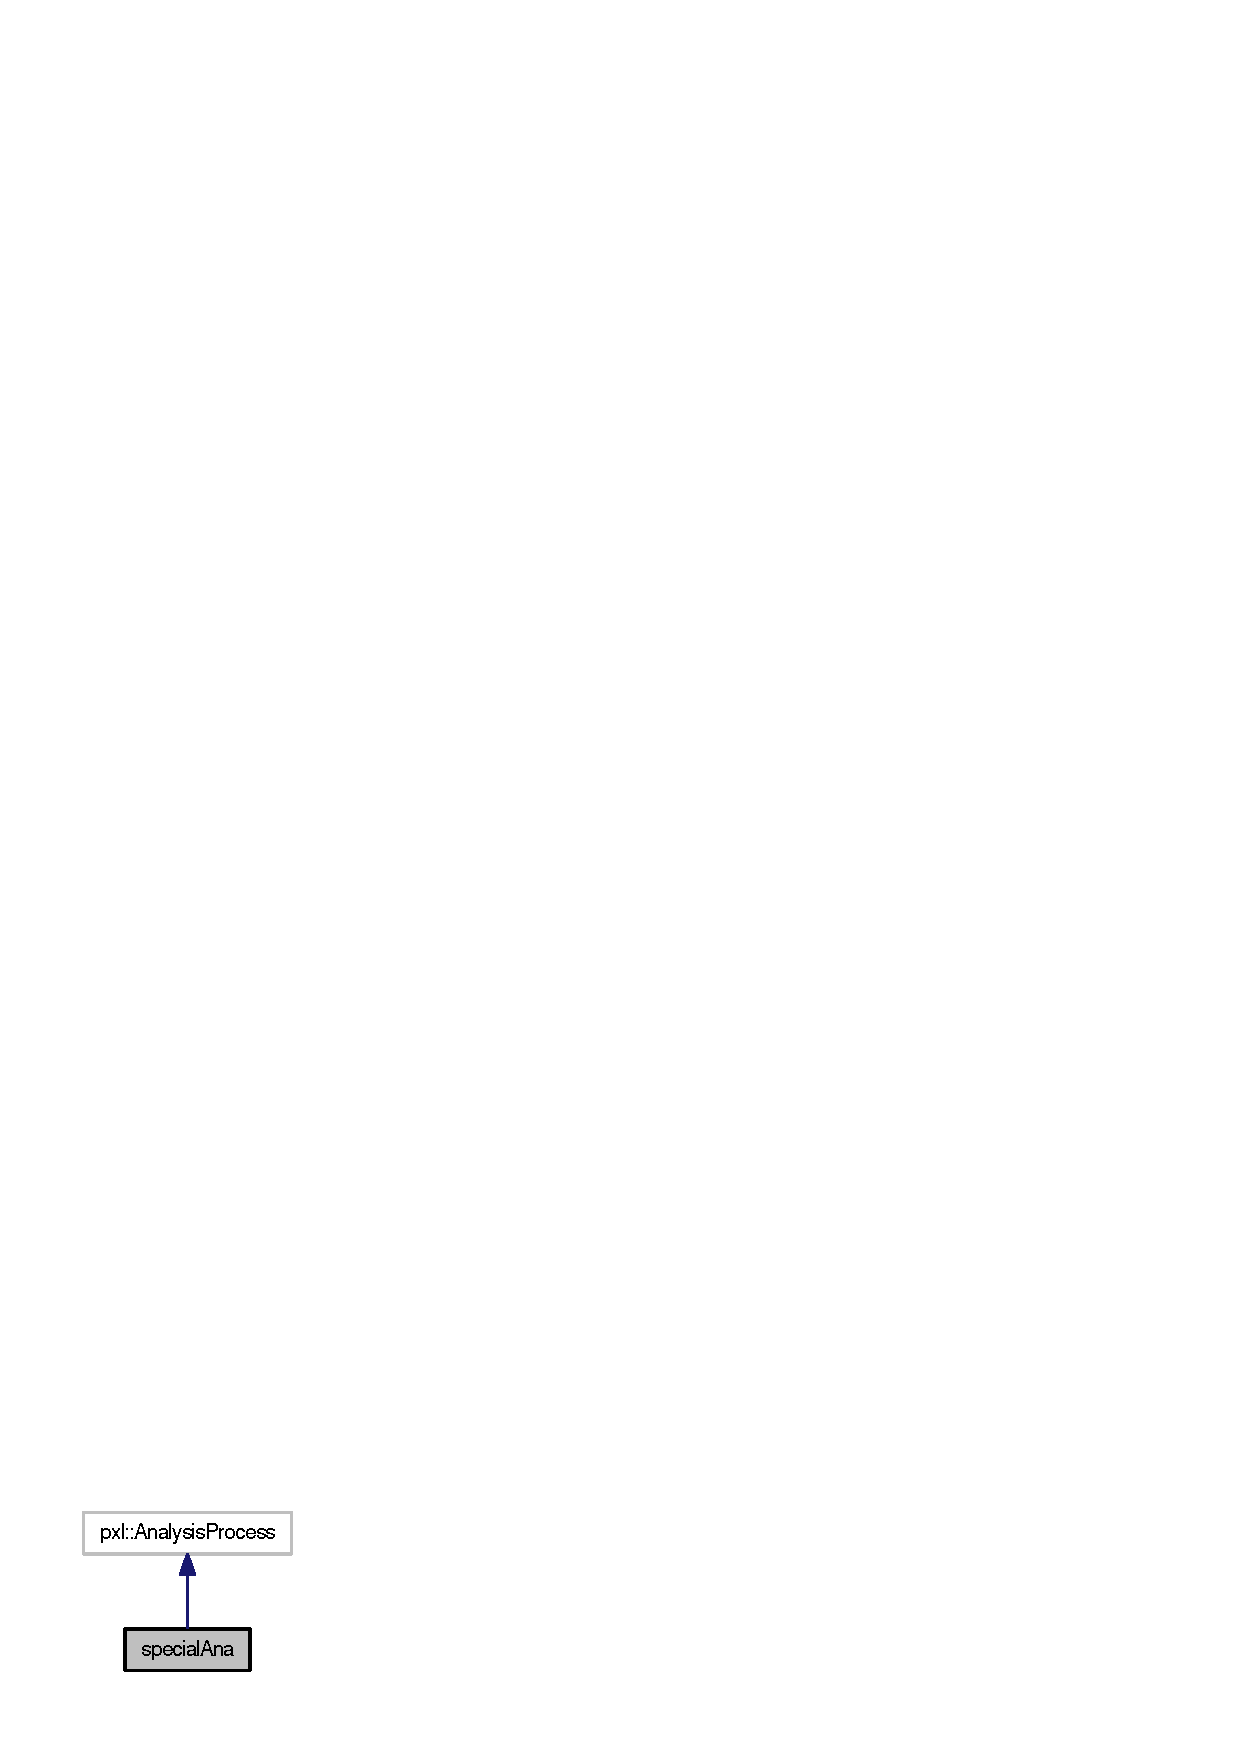
\includegraphics[width=144pt]{classspecialAna__inherit__graph}
\end{center}
\end{figure}


Collaboration diagram for special\-Ana\-:\nopagebreak
\begin{figure}[H]
\begin{center}
\leavevmode
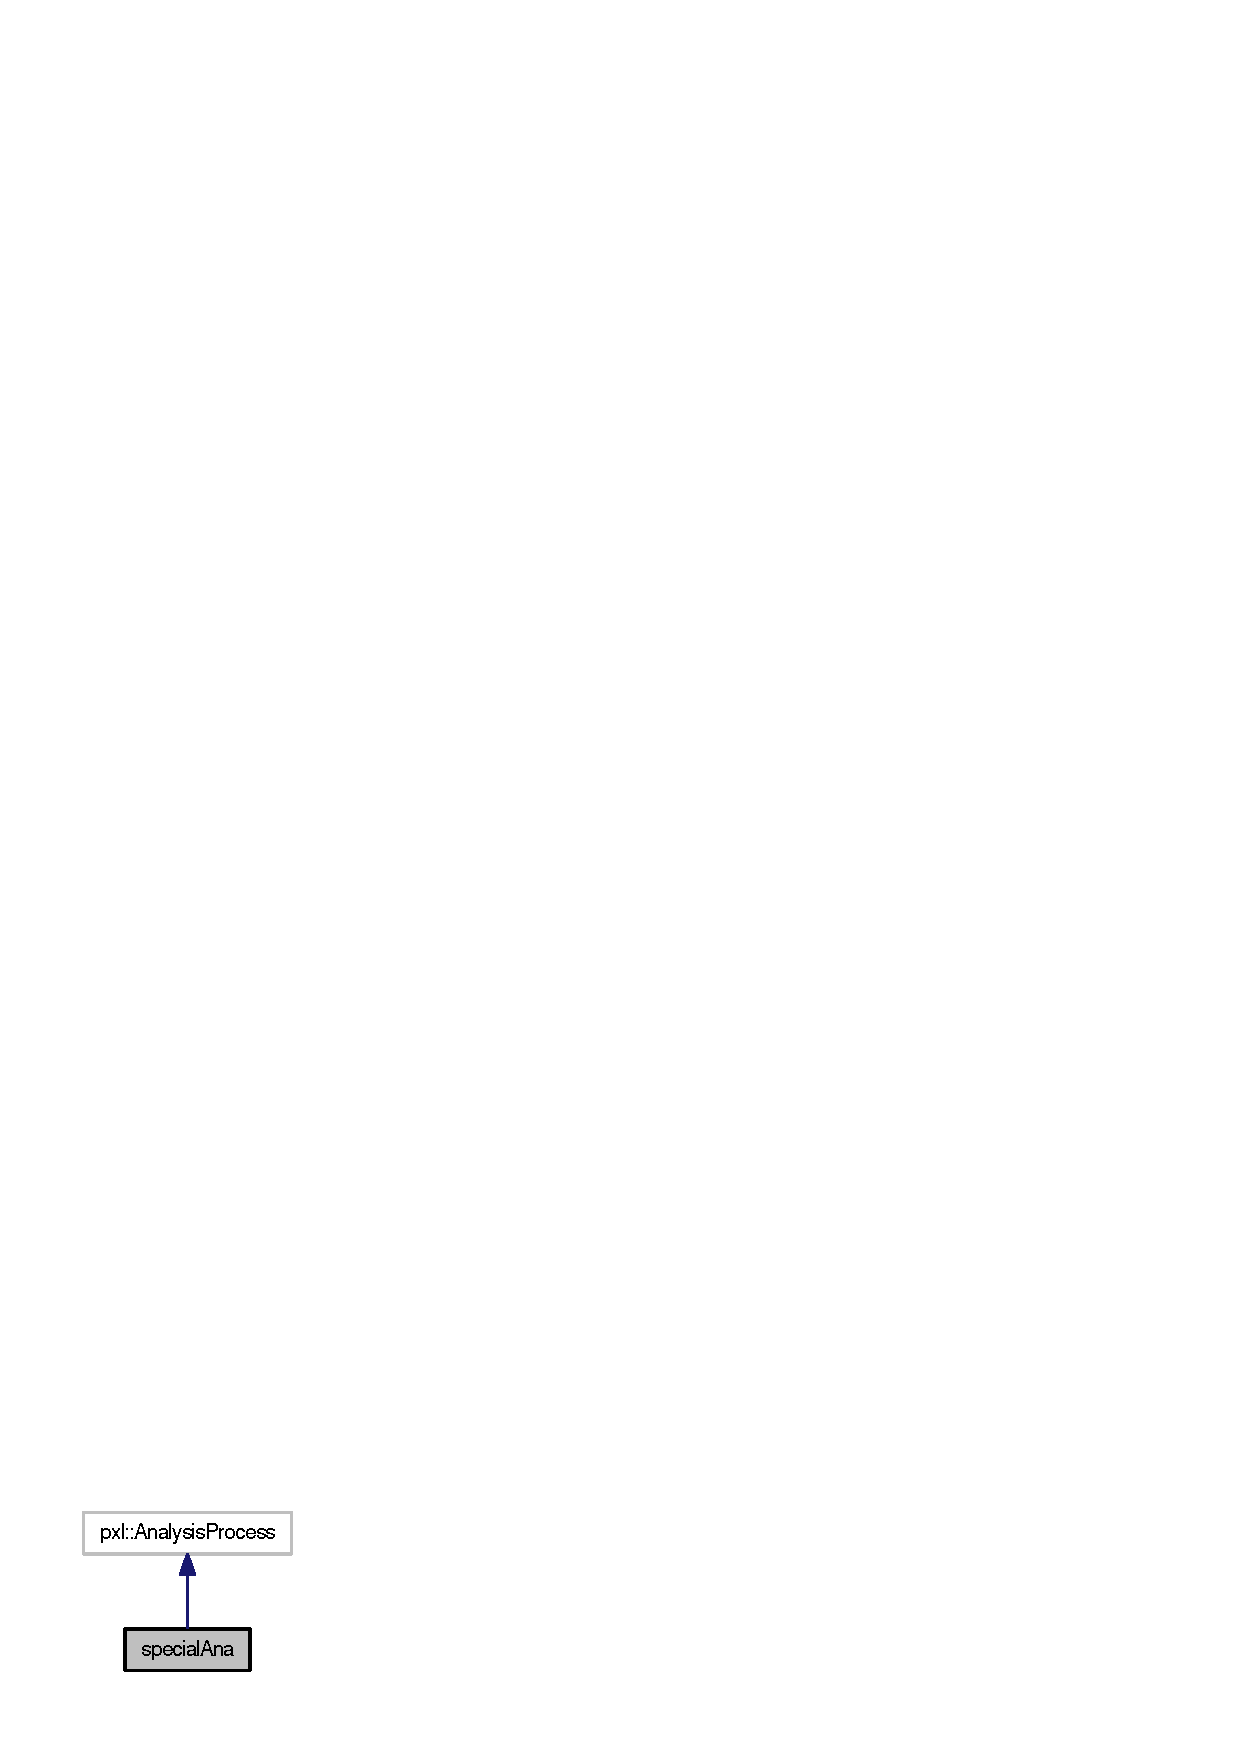
\includegraphics[width=144pt]{classspecialAna__coll__graph}
\end{center}
\end{figure}
\subsection*{Public Member Functions}
\begin{DoxyCompactItemize}
\item 
\hyperlink{classspecialAna_a709d6c8713ad2e1c14a13e384b14c21c}{special\-Ana} (const Tools\-::\-M\-Config \&config)
\item 
virtual \hyperlink{classspecialAna_aaeb00d6347026bf1ed542741f9b94ba0}{$\sim$special\-Ana} ()
\item 
virtual void \hyperlink{classspecialAna_a37d687c2af0195b3517fef360f98c979}{end\-Job} (const Serializable $\ast$)
\item 
virtual void \hyperlink{classspecialAna_a7de3fd03cce6954d6fdea113eac64799}{analyse\-Event} (const pxl\-::\-Event $\ast$event)
\item 
void \hyperlink{classspecialAna_a6a64568748075d84318c3a94731431b4}{channel\-\_\-writer} (T\-File $\ast$file, const char $\ast$channel)
\item 
bool \hyperlink{classspecialAna_ac1c57a46908e05ba036a0d876a01d805}{tail\-\_\-selector} (const pxl\-::\-Event $\ast$event)
\item 
void \hyperlink{classspecialAna_a67e68ba192d60a50835f0542b828d9ec}{Create\-\_\-\-Gen\-\_\-histograms} (const char $\ast$channel, const char $\ast$part1, const char $\ast$part2)
\item 
void \hyperlink{classspecialAna_ac84e4d445770d092d3eabb1190a7f9bc}{Fill\-\_\-\-Gen\-\_\-histograms} (const char $\ast$channel, const char $\ast$part1, const char $\ast$part2)
\item 
void \hyperlink{classspecialAna_a6e6b80f16fbb84dba1ff7f8245938164}{Init\-\_\-emu\-\_\-cuts} ()
\item 
void \hyperlink{classspecialAna_a6fa51ec65238915bb415ad7f7d63767b}{Init\-\_\-etau\-\_\-cuts} ()
\item 
void \hyperlink{classspecialAna_a7700dad4d41222c7dfb66e34da83ef3e}{Init\-\_\-mutau\-\_\-cuts} ()
\item 
void \hyperlink{classspecialAna_a8e01b23b113658e9c1f978eea69a39ef}{Init\-\_\-etaue\-\_\-cuts} ()
\item 
void \hyperlink{classspecialAna_a5fff5c84a270e73d3883bf1fb0a61b33}{Init\-\_\-etaumu\-\_\-cuts} ()
\item 
void \hyperlink{classspecialAna_ad63394b3c2396acdccadf5eeffa6fa83}{Init\-\_\-mutaue\-\_\-cuts} ()
\item 
void \hyperlink{classspecialAna_ad065f19da9d982699fb105d1670bb47e}{Init\-\_\-mutaumu\-\_\-cuts} ()
\item 
void \hyperlink{classspecialAna_a5a8d03afb432c7ce987b7d319cf475c4}{Fill\-Controll\-Histos} ()
\item 
void \hyperlink{classspecialAna_a24c1665cec24295951bb4a78442fdd83}{Create\-\_\-\-N1\-\_\-histos} (const char $\ast$channel, std\-::map$<$ std\-::string, \hyperlink{classCuts}{Cuts} $>$ \&m\-\_\-cfg, std\-::string const endung=\char`\"{}\char`\"{})
\item 
void \hyperlink{classspecialAna_a3ebe8a8f452b201a078c460a3e052854}{Fill\-\_\-\-N1\-\_\-histos} (const char $\ast$channel, std\-::map$<$ std\-::string, \hyperlink{classCuts}{Cuts} $>$ \&m\-\_\-cfg, std\-::string const endung=\char`\"{}\char`\"{})
\item 
void \hyperlink{classspecialAna_a7be51543df2b4fcbe5d4ae802028fffb}{Create\-\_\-\-Resonance\-\_\-histograms} (int n\-\_\-histos, const char $\ast$channel, const char $\ast$part1, const char $\ast$part2, std\-::string const endung=\char`\"{}\char`\"{})
\item 
void \hyperlink{classspecialAna_ae2c14a5d38214aee793dd6801b66b2c8}{Fill\-\_\-\-Resonance\-\_\-histograms} (int n\-\_\-histos, const char $\ast$channel, const char $\ast$part1, const char $\ast$part2, std\-::string const endung=\char`\"{}\char`\"{})
\item 
void \hyperlink{classspecialAna_a16ba40b9f9d027a4bd26859fd13642fc}{Kinematics\-Selector} (std\-::string const endung=\char`\"{}\char`\"{})
\item 
bool \hyperlink{classspecialAna_a5f15a75ae1b9dee9633dc4243e60f0ea}{Find\-Resonance} (const char $\ast$channel, vector$<$ pxl\-::\-Particle $\ast$ $>$ gen\-\_\-list)
\item 
bool \hyperlink{classspecialAna_a114fc22f04da620313ccada3cc1cf412}{Find\-Resonance} (const char $\ast$channel, vector$<$ pxl\-::\-Particle $\ast$ $>$ part1\-\_\-list, vector$<$ pxl\-::\-Particle $\ast$ $>$ part2\-\_\-list)
\item 
bool \hyperlink{classspecialAna_a897bc49eeef23f5982d4d6adadb3837b}{Find\-Resonance} (const char $\ast$channel, vector$<$ pxl\-::\-Particle $\ast$ $>$ part1\-\_\-list, vector$<$ pxl\-::\-Particle $\ast$ $>$ part2\-\_\-list, vector$<$ pxl\-::\-Particle $\ast$ $>$ met\-\_\-list)
\item 
void \hyperlink{classspecialAna_a1910a5c4831d81dd596b192231579994}{Gen\-Selector} ()
\item 
void \hyperlink{classspecialAna_a9ddbb4b17312c5eb0def21037db6eb93}{Fill\-\_\-\-Gen\-\_\-\-Controll\-\_\-histo} ()
\item 
void \hyperlink{classspecialAna_a9c41a6185342e9e612796dc8e35cafaf}{Fill\-\_\-\-Particle\-\_\-histos} (int hist\-\_\-number, pxl\-::\-Particle $\ast$lepton)
\item 
void \hyperlink{classspecialAna_abdfb375e586c5403addc11fd579740ea}{Fill\-\_\-\-Gen\-\_\-histograms} (int n\-\_\-histos, const char $\ast$channel, const char $\ast$part1, const char $\ast$part2)
\item 
pxl\-::\-Particle $\ast$ \hyperlink{classspecialAna_a29be2d17ee48fc508fa2dd9dc7f09762}{Get\-\_\-\-Truth\-\_\-match} (string name, pxl\-::\-Particle $\ast$lepton)
\item 
void \hyperlink{classspecialAna_ab0c365edd2b99787852a8ca21b612672}{Fill\-Systematics} (const pxl\-::\-Event $\ast$event, std\-::string const particle\-Name)
\item 
void \hyperlink{classspecialAna_a2233cf73756ab1135592eda1daeb45e5}{Fill\-Systematics\-Up\-Down} (const pxl\-::\-Event $\ast$event, std\-::string const particle\-Name, std\-::string const updown, std\-::string const shift\-Type)
\item 
void \hyperlink{classspecialAna_a0dbcc8ff0def8509792f0256cbbad85e}{init\-Event} (const pxl\-::\-Event $\ast$event)
\item 
void \hyperlink{classspecialAna_a0f73f64ce2c3e2c50c822a006ba680c1}{end\-Event} (const pxl\-::\-Event $\ast$event)
\item 
bool \hyperlink{classspecialAna_a3da70eb8be6a5ccdf1e5566ccf275aed}{Check\-\_\-\-Par\-\_\-\-I\-D} (pxl\-::\-Particle $\ast$part)
\item 
bool \hyperlink{classspecialAna_aeb000115550c29442092ee8567970124}{Check\-\_\-\-Muo\-\_\-\-I\-D} (pxl\-::\-Particle $\ast$muon)
\item 
bool \hyperlink{classspecialAna_ae78625a0c42a7e30927996f4117ed2f5}{Check\-\_\-\-Tau\-\_\-\-I\-D} (pxl\-::\-Particle $\ast$tau)
\item 
bool \hyperlink{classspecialAna_a8ddbe8fd55d1f44ef6842bdea591fa0f}{Check\-\_\-\-Ele\-\_\-\-I\-D} (pxl\-::\-Particle $\ast$ele)
\item 
vector$<$ double $>$ \hyperlink{classspecialAna_afe8814caa57ef3d373cd16f34e10494a}{Make\-\_\-zeta\-\_\-stuff} (pxl\-::\-Particle $\ast$muon, pxl\-::\-Particle $\ast$tau, pxl\-::\-Particle $\ast$met)
\item 
bool \hyperlink{classspecialAna_a6ecfdf37feacbf9b285a521edcdca579}{Make\-\_\-zeta\-\_\-cut} (\hyperlink{classCuts}{Cuts} \&cuts)
\item 
bool \hyperlink{classspecialAna_a977d93938993f07d68c995d0b6b93f5e}{Make\-\_\-\-Delta\-Phi\-\_\-tau\-M\-E\-T} (\hyperlink{classCuts}{Cuts} \&cuts)
\item 
bool \hyperlink{classspecialAna_aebff8eb590cd7facedac62b7f92fe0a4}{Make\-\_\-\-Delta\-Phi\-\_\-mutau} (\hyperlink{classCuts}{Cuts} \&cuts)
\item 
bool \hyperlink{classspecialAna_a4ee793e1dd340b2d82928a62a207cc8b}{Make\-\_\-\-Delta\-Phi\-\_\-tauemu} (\hyperlink{classCuts}{Cuts} \&cuts)
\item 
bool \hyperlink{classspecialAna_ac0e1d88ebff2ec0899b721e7c3ca2b0e}{Bjet\-\_\-veto} (\hyperlink{classCuts}{Cuts} \&cuts)
\item 
bool \hyperlink{classspecialAna_a00234e58c40f7c972287d1f06d17b547}{Opp\-Sign\-\_\-charge} (\hyperlink{classCuts}{Cuts} \&cuts)
\item 
bool \hyperlink{classspecialAna_a488e0e15a436a9ed877718101eb70ce4}{M\-T\-\_\-cut} (\hyperlink{classCuts}{Cuts} \&cuts)
\item 
double \hyperlink{classspecialAna_a1829be6b0581ef1d46258163466a899b}{calc\-\_\-lep\-\_\-fraction} ()
\item 
bool \hyperlink{classspecialAna_a5eba4cc7dd4f309946b1bcf79259b098}{Leptonic\-\_\-fraction\-\_\-cut} (\hyperlink{classCuts}{Cuts} \&cuts)
\item 
bool \hyperlink{classspecialAna_ae106d787dd2453faba4bfa0a99cb3253}{p\-T\-\_\-mutau\-\_\-ratio\-\_\-cut} (\hyperlink{classCuts}{Cuts} \&cuts)
\item 
bool \hyperlink{classspecialAna_abc40177d37851dc68b4fd8c9609a23a7}{p\-T\-\_\-muele\-\_\-ratio\-\_\-cut} (\hyperlink{classCuts}{Cuts} \&cuts)
\item 
bool \hyperlink{classspecialAna_a6f96f4a11c793dcc97e530cd5ff245a2}{Make\-\_\-\-Delta\-Phi\-\_\-emu} (\hyperlink{classCuts}{Cuts} \&cuts)
\item 
bool \hyperlink{classspecialAna_a28a598e3f0ef500d0d2171751fdfd842}{Trigger\-Selector} (const pxl\-::\-Event $\ast$event)
\item 
double \hyperlink{classspecialAna_a13633015e15fd8354abadae9b07a4a3a}{Delta\-Phi} (double a, double b)
\item 
double \hyperlink{classspecialAna_ae6b596bc1040d602298b5d0501abb13d}{Delta\-Phi} (pxl\-::\-Particle $\ast$lepton, pxl\-::\-Particle $\ast$met)
\item 
double \hyperlink{classspecialAna_af80d7455d04539410714b947025f4bf4}{M\-T} (pxl\-::\-Particle $\ast$lepton, pxl\-::\-Particle $\ast$met)
\item 
double \hyperlink{classspecialAna_ac6dc740c484c3291b7c8e4d707c109dc}{get\-Pt\-Hat} ()
\item 
double \hyperlink{classspecialAna_ab358fee251f1dc54cdf046e898361d83}{get\-H\-T} ()
\end{DoxyCompactItemize}
\subsection*{Public Attributes}
\begin{DoxyCompactItemize}
\item 
T\-File $\ast$ \hyperlink{classspecialAna_a926d4b22d2a4c69f67ad9a2708ae96a0}{file1}
\item 
pxl\-::\-Event\-View $\ast$ \hyperlink{classspecialAna_a7544fa663090f43e35ff6c8594884c37}{m\-\_\-\-Rec\-Evt\-View}
\item 
pxl\-::\-Event\-View $\ast$ \hyperlink{classspecialAna_a68771d0c3f87434532645d27d5c2316b}{m\-\_\-\-Gen\-Evt\-View}
\item 
pxl\-::\-Event\-View $\ast$ \hyperlink{classspecialAna_aaacff41e1aa1c73726d348ead1319c2e}{m\-\_\-\-Trig\-Evt\-View}
\item 
bool \hyperlink{classspecialAna_aad40cb68a6bfb77e015fd348b620fa4a}{run\-On\-Data}
\item 
string const \hyperlink{classspecialAna_a7ac446797f2e7984a748e887709870c3}{m\-\_\-\-Jet\-Algo}
\item 
string const \hyperlink{classspecialAna_adf4b91d17a05add2c475bad5ab72d414}{m\-\_\-\-B\-Jets\-\_\-algo}
\item 
string const \hyperlink{classspecialAna_a3463aa545f96fc9a4ae14b82aadb01c6}{m\-\_\-\-M\-E\-T\-Type}
\item 
string const \hyperlink{classspecialAna_a928cc6c577c7d2a9df708f038c7b7b2f}{m\-\_\-\-Tau\-Type}
\item 
const std\-::string \hyperlink{classspecialAna_a68eaaa795a5c08f7505d44b51361b224}{particles} \mbox{[}4\mbox{]} = \{\char`\"{}Ele\char`\"{}, \char`\"{}Muon\char`\"{}, \char`\"{}Tau\char`\"{}, \char`\"{}M\-E\-T\char`\"{}\}
\item 
const std\-::string \hyperlink{classspecialAna_a5500b6ed6706afbab4721747b9a475c8}{particle\-Symbols} \mbox{[}4\mbox{]} = \{\char`\"{}e\char`\"{}, \char`\"{}\#mu\char`\"{}, \char`\"{}\#tau\char`\"{}, \char`\"{}E\-\_\-\{T\}$^\wedge$\{miss\}\char`\"{}\}
\item 
T\-String \hyperlink{classspecialAna_a6b83298c41f32cdbd7979ec8033eefd6}{d\-\_\-mydisc} \mbox{[}66\mbox{]}
\item 
bool \hyperlink{classspecialAna_add184c9cd673ecf710b3801749931b03}{is\-Old\-P\-X\-L\-File}
\item 
const std\-::string \hyperlink{classspecialAna_aac185c43fcd3fbaa8b869fb8bdba8b42}{m\-\_\-cutdatafile}
\item 
const vector$<$ string $>$ \hyperlink{classspecialAna_a4e5b506555aa75a4b132df95398a5ae5}{m\-\_\-trigger\-\_\-string}
\item 
T\-String \hyperlink{classspecialAna_a8bd00db3975c79baf92da5f720cca2fc}{d\-\_\-mydiscmu} \mbox{[}6\mbox{]}
\item 
const std\-::string \hyperlink{classspecialAna_a5962acc8cee4aa0fdb0f01caab08dd22}{m\-\_\-data\-Period}
\item 
const std\-::string \hyperlink{classspecialAna_a71e9557d5927332677564f33668e8c80}{m\-\_\-channel}
\item 
const Tools\-::\-M\-Config \hyperlink{classspecialAna_a1e76bd61bb4a97d99729f398674e14e2}{config\-\_\-}
\item 
double \hyperlink{classspecialAna_a739ec443ba622f962854c133080624db}{temp\-\_\-run}
\item 
double \hyperlink{classspecialAna_ad1c4dd4e6eb56e86c4ad24b8f942ebef}{temp\-\_\-ls}
\item 
double \hyperlink{classspecialAna_a70360bfdefab8b0cdfd126e40d109c34}{temp\-\_\-event}
\item 
double \hyperlink{classspecialAna_a093be544141cb52a9b5a1f5ef3bb7e32}{weight}
\item 
unsigned int \hyperlink{classspecialAna_af9324bf8986d292f34deeb070d0eccb1}{num\-Muon}
\item 
unsigned int \hyperlink{classspecialAna_a11b4167816b835bd2a729ebde0dc1098}{num\-Ele}
\item 
unsigned int \hyperlink{classspecialAna_a3f9a479af1480789df7ac7978b61cca5}{num\-Tau}
\item 
unsigned int \hyperlink{classspecialAna_a76c852b99af4a8890ab656c041fba8af}{num\-Gamma}
\item 
unsigned int \hyperlink{classspecialAna_a13da6896f59e970912c902579e3887e5}{num\-M\-E\-T}
\item 
unsigned int \hyperlink{classspecialAna_aa2601aeefa3374b37708442a41f9d876}{num\-Jet}
\item 
unsigned int \hyperlink{classspecialAna_af82a39567ee3dd6a4e5f5bfd439e3945}{num\-B\-Jet}
\item 
int \hyperlink{classspecialAna_aff5d8d0f950637c1d885ebfff0c3b9a8}{events\-\_\-}
\item 
unsigned int \hyperlink{classspecialAna_af80eb340f7aed6a1d0caa49d2b30a884}{n\-\_\-lepton}
\item 
vector$<$ pxl\-::\-Particle $\ast$ $>$ $\ast$ \hyperlink{classspecialAna_a20428604e5f83134e03ded624a4f4c6a}{Ele\-List}
\item 
vector$<$ pxl\-::\-Particle $\ast$ $>$ $\ast$ \hyperlink{classspecialAna_a6bcf2c30750671faeda4f4b38a4cfbb7}{Muon\-List}
\item 
vector$<$ pxl\-::\-Particle $\ast$ $>$ $\ast$ \hyperlink{classspecialAna_a84140461ae32bd6482b36642714d2669}{Tau\-List}
\item 
vector$<$ pxl\-::\-Particle $\ast$ $>$ $\ast$ \hyperlink{classspecialAna_ae66ed155895258a7dbbf3cc1d89a8e26}{Gamma\-List}
\item 
vector$<$ pxl\-::\-Particle $\ast$ $>$ $\ast$ \hyperlink{classspecialAna_a26e3e78376bd7d09a09d6b2db1152402}{M\-E\-T\-List}
\item 
vector$<$ pxl\-::\-Particle $\ast$ $>$ $\ast$ \hyperlink{classspecialAna_a3d7eb132203a986d49e303ba8cdd606f}{Jet\-List}
\item 
vector$<$ pxl\-::\-Particle $\ast$ $>$ $\ast$ \hyperlink{classspecialAna_a2978a50df2e166bb5475200bff24ffb2}{B\-Jet\-List}
\item 
vector$<$ pxl\-::\-Particle $\ast$ $>$ $\ast$ \hyperlink{classspecialAna_a803a475f188fbbe83b866ced8ece1442}{Remember\-Part}
\item 
vector$<$ pxl\-::\-Particle $\ast$ $>$ $\ast$ \hyperlink{classspecialAna_a3da2afad197768ff70017d2439a4ecbb}{Remember\-M\-E\-T}
\item 
vector$<$ pxl\-::\-Particle $\ast$ $>$ $\ast$ \hyperlink{classspecialAna_a8bfd838b3d91f8a0721b22b75c4078a9}{Ele\-List\-Gen}
\item 
vector$<$ pxl\-::\-Particle $\ast$ $>$ $\ast$ \hyperlink{classspecialAna_ab7b983c53e3c9bc2f4677fc76ef65fb0}{Muon\-List\-Gen}
\item 
vector$<$ pxl\-::\-Particle $\ast$ $>$ $\ast$ \hyperlink{classspecialAna_a4d474151b634aefba1f87728805d45fe}{Tau\-List\-Gen}
\item 
vector$<$ pxl\-::\-Particle $\ast$ $>$ $\ast$ \hyperlink{classspecialAna_a1e4de01edc121633e4c961284def2ef3}{Gamma\-List\-Gen}
\item 
vector$<$ pxl\-::\-Particle $\ast$ $>$ $\ast$ \hyperlink{classspecialAna_a771b064c24368a06e5de930cb48f2d36}{M\-E\-T\-List\-Gen}
\item 
vector$<$ pxl\-::\-Particle $\ast$ $>$ $\ast$ \hyperlink{classspecialAna_aaab9fa9e1d1e85bc1ff931569a709096}{Jet\-List\-Gen}
\item 
vector$<$ pxl\-::\-Particle $\ast$ $>$ $\ast$ \hyperlink{classspecialAna_a401eeadc9b34b0278c2cdf45256e9baa}{S3\-List\-Gen}
\item 
bool \hyperlink{classspecialAna_abcfabe97f1d18a464f420c1b47582338}{b\-\_\-14\-Te\-V}
\item 
bool \hyperlink{classspecialAna_aa8d4b44be61d1e2f53c63a5dfb42382d}{b\-\_\-13\-Te\-V}
\item 
bool \hyperlink{classspecialAna_ac4ed94b197d05282ab2aeed78bea4dad}{b\-\_\-8\-Te\-V}
\item 
bool \hyperlink{classspecialAna_aae4e34dea84468db09355f5c33ac58dd}{b\-\_\-emu}
\item 
bool \hyperlink{classspecialAna_a14aecaa955dbd8cb22e22107c1991ebe}{b\-\_\-etau}
\item 
bool \hyperlink{classspecialAna_ae6b84e17047e8a379fad795966129512}{b\-\_\-mutau}
\item 
bool \hyperlink{classspecialAna_ab6038122295663c5a43fe1e89c86ae36}{b\-\_\-etaue}
\item 
bool \hyperlink{classspecialAna_a1ea533f85d436109263a69b2943b906b}{b\-\_\-etaumu}
\item 
bool \hyperlink{classspecialAna_a3b8dec739eeb3aba67512a275a740978}{b\-\_\-mutaue}
\item 
bool \hyperlink{classspecialAna_a251c50e90dd2f85e67dac70abd219bf9}{b\-\_\-mutaumu}
\item 
map$<$ string, \hyperlink{classCuts}{Cuts} $>$ \hyperlink{classspecialAna_a15d1b215f95e104a1728a3e090ef76df}{emu\-\_\-cut\-\_\-cfgs}
\item 
map$<$ string, \hyperlink{classCuts}{Cuts} $>$ \hyperlink{classspecialAna_aae200ba5c12c48ca4dadc47e657a14fc}{etau\-\_\-cut\-\_\-cfgs}
\item 
map$<$ string, \hyperlink{classCuts}{Cuts} $>$ \hyperlink{classspecialAna_a1cc60d87fb53c47860a45b50f996147f}{mutau\-\_\-cut\-\_\-cfgs}
\item 
map$<$ string, \hyperlink{classCuts}{Cuts} $>$ \hyperlink{classspecialAna_abd425daefdae175f64d5d2ec8eaeb859}{etaue\-\_\-cut\-\_\-cfgs}
\item 
map$<$ string, \hyperlink{classCuts}{Cuts} $>$ \hyperlink{classspecialAna_a649fbc7d8b73e8227e7844a3d7d2f7d5}{etaumu\-\_\-cut\-\_\-cfgs}
\item 
map$<$ string, \hyperlink{classCuts}{Cuts} $>$ \hyperlink{classspecialAna_ae140f6e63d9061ce6b8310f093e163c6}{mutaue\-\_\-cut\-\_\-cfgs}
\item 
map$<$ string, \hyperlink{classCuts}{Cuts} $>$ \hyperlink{classspecialAna_af9e77720216d2b89101572b8b620ab72}{mutaumu\-\_\-cut\-\_\-cfgs}
\item 
map$<$ string, int $>$ \hyperlink{classspecialAna_a58cbc80a0bb41446344e4d9170450974}{channel\-\_\-stages}
\item 
pxl\-::\-Particle $\ast$ \hyperlink{classspecialAna_a9beb30fa9c4671d0b5d6a35df0470fa8}{sel\-\_\-part1\-\_\-gen}
\item 
pxl\-::\-Particle $\ast$ \hyperlink{classspecialAna_a5e06d3c9b3b9dbd2353e7abf1645d32e}{sel\-\_\-part2\-\_\-gen}
\item 
pxl\-::\-Particle $\ast$ \hyperlink{classspecialAna_aee9025a3b86abbffe066e42aa521d801}{sel\-\_\-lepton\-\_\-prompt}
\item 
pxl\-::\-Particle $\ast$ \hyperlink{classspecialAna_a2bb3bd3f562063bd54fa72eb36a4d7de}{sel\-\_\-lepton\-\_\-nprompt}
\item 
pxl\-::\-Particle $\ast$ \hyperlink{classspecialAna_adf5da0cbdfda1f8b7e2504cdd3506ba0}{sel\-\_\-met}
\item 
pxl\-::\-Particle $\ast$ \hyperlink{classspecialAna_aa92d86a2b74ba4f7157522752e638a22}{sel\-\_\-lepton\-\_\-nprompt\-\_\-corr}
\item 
map$<$ string, double $>$ \hyperlink{classspecialAna_a1af23a7951217b703465b152e08d8ec6}{resonance\-\_\-mass}
\item 
map$<$ string, double $>$ \hyperlink{classspecialAna_aa0c7fe4e8cb8142f2f8f4c4967e658b2}{resonance\-\_\-mass\-\_\-gen}
\item 
unordered\-\_\-set$<$ string $>$ \hyperlink{classspecialAna_a7578000c63d8e3555315047763358e32}{triggers}
\item 
map$<$ string, float $>$ \hyperlink{classspecialAna_ae7c181ead078f2fec53d80943afe9352}{m\-Lepton\-Tree}
\item 
bool \hyperlink{classspecialAna_affbbcba600d494b2dbb3397bea059672}{keep\-\_\-data\-\_\-event}
\item 
map$<$ string, float $>$ \hyperlink{classspecialAna_a94f42f297f53448b135d5586055bb7d1}{mkeep\-\_\-resonance\-\_\-mass}
\item 
double \hyperlink{classspecialAna_aaafb641b3e4372a247d24b678ed4a549}{event\-\_\-weight}
\item 
double \hyperlink{classspecialAna_a2b5b5144746c7a945308b1700a0b0a10}{pileup\-\_\-weight}
\item 
T\-Efficiency $\ast$ \hyperlink{classspecialAna_a1271615b07b243df0bd09c1c612258af}{p\-Eff}
\end{DoxyCompactItemize}


\subsection{Detailed Description}


Definition at line 30 of file special\-Ana.\-hh.



\subsection{Constructor \& Destructor Documentation}
\index{special\-Ana@{special\-Ana}!special\-Ana@{special\-Ana}}
\index{special\-Ana@{special\-Ana}!specialAna@{special\-Ana}}
\subsubsection[{special\-Ana}]{\setlength{\rightskip}{0pt plus 5cm}special\-Ana\-::special\-Ana (
\begin{DoxyParamCaption}
\item[{const Tools\-::\-M\-Config \&}]{config}
\end{DoxyParamCaption}
)}\label{classspecialAna_a709d6c8713ad2e1c14a13e384b14c21c}


Definition at line 10 of file special\-Ana.\-cc.

\index{special\-Ana@{special\-Ana}!$\sim$special\-Ana@{$\sim$special\-Ana}}
\index{$\sim$special\-Ana@{$\sim$special\-Ana}!specialAna@{special\-Ana}}
\subsubsection[{$\sim$special\-Ana}]{\setlength{\rightskip}{0pt plus 5cm}special\-Ana\-::$\sim$special\-Ana (
\begin{DoxyParamCaption}
{}
\end{DoxyParamCaption}
)\hspace{0.3cm}{\ttfamily [virtual]}}\label{classspecialAna_aaeb00d6347026bf1ed542741f9b94ba0}


Definition at line 278 of file special\-Ana.\-cc.



\subsection{Member Function Documentation}
\index{special\-Ana@{special\-Ana}!analyse\-Event@{analyse\-Event}}
\index{analyse\-Event@{analyse\-Event}!specialAna@{special\-Ana}}
\subsubsection[{analyse\-Event}]{\setlength{\rightskip}{0pt plus 5cm}void special\-Ana\-::analyse\-Event (
\begin{DoxyParamCaption}
\item[{const pxl\-::\-Event $\ast$}]{event}
\end{DoxyParamCaption}
)\hspace{0.3cm}{\ttfamily [virtual]}}\label{classspecialAna_a7de3fd03cce6954d6fdea113eac64799}


Definition at line 281 of file special\-Ana.\-cc.



References Check\-\_\-\-Muo\-\_\-\-I\-D(), Check\-\_\-\-Tau\-\_\-\-I\-D(), Ele\-List, end\-Event(), Fill\-\_\-\-Gen\-\_\-\-Controll\-\_\-histo(), Fill\-\_\-\-Particle\-\_\-histos(), Fill\-Controll\-Histos(), Fill\-Systematics(), Fill\-Systematics\-Up\-Down(), Gen\-Selector(), init\-Event(), Kinematics\-Selector(), M\-E\-T\-List, Muon\-List, p\-Eff, run\-On\-Data, tail\-\_\-selector(), Tau\-List, Trigger\-Selector(), and weight.

\index{special\-Ana@{special\-Ana}!Bjet\-\_\-veto@{Bjet\-\_\-veto}}
\index{Bjet\-\_\-veto@{Bjet\-\_\-veto}!specialAna@{special\-Ana}}
\subsubsection[{Bjet\-\_\-veto}]{\setlength{\rightskip}{0pt plus 5cm}bool special\-Ana\-::\-Bjet\-\_\-veto (
\begin{DoxyParamCaption}
\item[{{\bf Cuts} \&}]{cuts}
\end{DoxyParamCaption}
)}\label{classspecialAna_ac0e1d88ebff2ec0899b721e7c3ca2b0e}


Definition at line 1417 of file special\-Ana.\-cc.



References num\-B\-Jet, and Cuts\-::\-Set\-Vars().



Referenced by Kinematics\-Selector().

\index{special\-Ana@{special\-Ana}!calc\-\_\-lep\-\_\-fraction@{calc\-\_\-lep\-\_\-fraction}}
\index{calc\-\_\-lep\-\_\-fraction@{calc\-\_\-lep\-\_\-fraction}!specialAna@{special\-Ana}}
\subsubsection[{calc\-\_\-lep\-\_\-fraction}]{\setlength{\rightskip}{0pt plus 5cm}double special\-Ana\-::calc\-\_\-lep\-\_\-fraction (
\begin{DoxyParamCaption}
{}
\end{DoxyParamCaption}
)}\label{classspecialAna_a1829be6b0581ef1d46258163466a899b}


Definition at line 1453 of file special\-Ana.\-cc.



References Jet\-List, sel\-\_\-lepton\-\_\-nprompt, and sel\-\_\-lepton\-\_\-prompt.



Referenced by Leptonic\-\_\-fraction\-\_\-cut().

\index{special\-Ana@{special\-Ana}!channel\-\_\-writer@{channel\-\_\-writer}}
\index{channel\-\_\-writer@{channel\-\_\-writer}!specialAna@{special\-Ana}}
\subsubsection[{channel\-\_\-writer}]{\setlength{\rightskip}{0pt plus 5cm}void special\-Ana\-::channel\-\_\-writer (
\begin{DoxyParamCaption}
\item[{T\-File $\ast$}]{file, }
\item[{const char $\ast$}]{channel}
\end{DoxyParamCaption}
)}\label{classspecialAna_a6a64568748075d84318c3a94731431b4}


Definition at line 1715 of file special\-Ana.\-cc.



References channel\-\_\-stages, and file1.



Referenced by end\-Job().

\index{special\-Ana@{special\-Ana}!Check\-\_\-\-Ele\-\_\-\-I\-D@{Check\-\_\-\-Ele\-\_\-\-I\-D}}
\index{Check\-\_\-\-Ele\-\_\-\-I\-D@{Check\-\_\-\-Ele\-\_\-\-I\-D}!specialAna@{special\-Ana}}
\subsubsection[{Check\-\_\-\-Ele\-\_\-\-I\-D}]{\setlength{\rightskip}{0pt plus 5cm}bool special\-Ana\-::\-Check\-\_\-\-Ele\-\_\-\-I\-D (
\begin{DoxyParamCaption}
\item[{pxl\-::\-Particle $\ast$}]{ele}
\end{DoxyParamCaption}
)}\label{classspecialAna_a8ddbe8fd55d1f44ef6842bdea591fa0f}


Definition at line 1316 of file special\-Ana.\-cc.



Referenced by Check\-\_\-\-Par\-\_\-\-I\-D().

\index{special\-Ana@{special\-Ana}!Check\-\_\-\-Muo\-\_\-\-I\-D@{Check\-\_\-\-Muo\-\_\-\-I\-D}}
\index{Check\-\_\-\-Muo\-\_\-\-I\-D@{Check\-\_\-\-Muo\-\_\-\-I\-D}!specialAna@{special\-Ana}}
\subsubsection[{Check\-\_\-\-Muo\-\_\-\-I\-D}]{\setlength{\rightskip}{0pt plus 5cm}bool special\-Ana\-::\-Check\-\_\-\-Muo\-\_\-\-I\-D (
\begin{DoxyParamCaption}
\item[{pxl\-::\-Particle $\ast$}]{muon}
\end{DoxyParamCaption}
)}\label{classspecialAna_aeb000115550c29442092ee8567970124}


Definition at line 1301 of file special\-Ana.\-cc.



References b\-\_\-13\-Te\-V, and b\-\_\-8\-Te\-V.



Referenced by analyse\-Event(), and Check\-\_\-\-Par\-\_\-\-I\-D().

\index{special\-Ana@{special\-Ana}!Check\-\_\-\-Par\-\_\-\-I\-D@{Check\-\_\-\-Par\-\_\-\-I\-D}}
\index{Check\-\_\-\-Par\-\_\-\-I\-D@{Check\-\_\-\-Par\-\_\-\-I\-D}!specialAna@{special\-Ana}}
\subsubsection[{Check\-\_\-\-Par\-\_\-\-I\-D}]{\setlength{\rightskip}{0pt plus 5cm}bool special\-Ana\-::\-Check\-\_\-\-Par\-\_\-\-I\-D (
\begin{DoxyParamCaption}
\item[{pxl\-::\-Particle $\ast$}]{part}
\end{DoxyParamCaption}
)}\label{classspecialAna_a3da70eb8be6a5ccdf1e5566ccf275aed}


Definition at line 1267 of file special\-Ana.\-cc.



References Check\-\_\-\-Ele\-\_\-\-I\-D(), Check\-\_\-\-Muo\-\_\-\-I\-D(), Check\-\_\-\-Tau\-\_\-\-I\-D(), and m\-\_\-\-Tau\-Type.



Referenced by Find\-Resonance().

\index{special\-Ana@{special\-Ana}!Check\-\_\-\-Tau\-\_\-\-I\-D@{Check\-\_\-\-Tau\-\_\-\-I\-D}}
\index{Check\-\_\-\-Tau\-\_\-\-I\-D@{Check\-\_\-\-Tau\-\_\-\-I\-D}!specialAna@{special\-Ana}}
\subsubsection[{Check\-\_\-\-Tau\-\_\-\-I\-D}]{\setlength{\rightskip}{0pt plus 5cm}bool special\-Ana\-::\-Check\-\_\-\-Tau\-\_\-\-I\-D (
\begin{DoxyParamCaption}
\item[{pxl\-::\-Particle $\ast$}]{tau}
\end{DoxyParamCaption}
)}\label{classspecialAna_ae78625a0c42a7e30927996f4117ed2f5}


Definition at line 1283 of file special\-Ana.\-cc.



References b\-\_\-13\-Te\-V, and b\-\_\-8\-Te\-V.



Referenced by analyse\-Event(), and Check\-\_\-\-Par\-\_\-\-I\-D().

\index{special\-Ana@{special\-Ana}!Create\-\_\-\-Gen\-\_\-histograms@{Create\-\_\-\-Gen\-\_\-histograms}}
\index{Create\-\_\-\-Gen\-\_\-histograms@{Create\-\_\-\-Gen\-\_\-histograms}!specialAna@{special\-Ana}}
\subsubsection[{Create\-\_\-\-Gen\-\_\-histograms}]{\setlength{\rightskip}{0pt plus 5cm}void special\-Ana\-::\-Create\-\_\-\-Gen\-\_\-histograms (
\begin{DoxyParamCaption}
\item[{const char $\ast$}]{channel, }
\item[{const char $\ast$}]{part1, }
\item[{const char $\ast$}]{part2}
\end{DoxyParamCaption}
)}\label{classspecialAna_a67e68ba192d60a50835f0542b828d9ec}
Resonant mass histogram

First particle histograms

Second particle histograms

Delta phi between the two particles

p\-T ratio of the two particles 

Definition at line 1003 of file special\-Ana.\-cc.

\index{special\-Ana@{special\-Ana}!Create\-\_\-\-N1\-\_\-histos@{Create\-\_\-\-N1\-\_\-histos}}
\index{Create\-\_\-\-N1\-\_\-histos@{Create\-\_\-\-N1\-\_\-histos}!specialAna@{special\-Ana}}
\subsubsection[{Create\-\_\-\-N1\-\_\-histos}]{\setlength{\rightskip}{0pt plus 5cm}void special\-Ana\-::\-Create\-\_\-\-N1\-\_\-histos (
\begin{DoxyParamCaption}
\item[{const char $\ast$}]{channel, }
\item[{std\-::map$<$ std\-::string, {\bf Cuts} $>$ \&}]{m\-\_\-cfg, }
\item[{std\-::string const}]{endung = {\ttfamily \char`\"{}\char`\"{}}}
\end{DoxyParamCaption}
)}\label{classspecialAna_a24c1665cec24295951bb4a78442fdd83}


Definition at line 923 of file special\-Ana.\-cc.

\index{special\-Ana@{special\-Ana}!Create\-\_\-\-Resonance\-\_\-histograms@{Create\-\_\-\-Resonance\-\_\-histograms}}
\index{Create\-\_\-\-Resonance\-\_\-histograms@{Create\-\_\-\-Resonance\-\_\-histograms}!specialAna@{special\-Ana}}
\subsubsection[{Create\-\_\-\-Resonance\-\_\-histograms}]{\setlength{\rightskip}{0pt plus 5cm}void special\-Ana\-::\-Create\-\_\-\-Resonance\-\_\-histograms (
\begin{DoxyParamCaption}
\item[{int}]{n\-\_\-histos, }
\item[{const char $\ast$}]{channel, }
\item[{const char $\ast$}]{part1, }
\item[{const char $\ast$}]{part2, }
\item[{std\-::string const}]{endung = {\ttfamily \char`\"{}\char`\"{}}}
\end{DoxyParamCaption}
)}\label{classspecialAna_a7be51543df2b4fcbe5d4ae802028fffb}
Cutflow histogram

Resonant mass histogram

Resonant mass resolution histogram

First particle histograms

Second particle histograms

Delta phi between the two particles

p\-T ratio of the two particles

Create histograms for channels with M\-E\-T

M\-E\-T histograms

Corrected second particle histogram

Delta phi between the other particles

p\-T ratio of the other particles 

Definition at line 1037 of file special\-Ana.\-cc.

\index{special\-Ana@{special\-Ana}!Delta\-Phi@{Delta\-Phi}}
\index{Delta\-Phi@{Delta\-Phi}!specialAna@{special\-Ana}}
\subsubsection[{Delta\-Phi}]{\setlength{\rightskip}{0pt plus 5cm}double special\-Ana\-::\-Delta\-Phi (
\begin{DoxyParamCaption}
\item[{double}]{a, }
\item[{double}]{b}
\end{DoxyParamCaption}
)}\label{classspecialAna_a13633015e15fd8354abadae9b07a4a3a}


Definition at line 1636 of file special\-Ana.\-cc.



Referenced by Fill\-\_\-\-Gen\-\_\-histograms(), Fill\-\_\-\-Resonance\-\_\-histograms(), Make\-\_\-\-Delta\-Phi\-\_\-emu(), Make\-\_\-\-Delta\-Phi\-\_\-mutau(), Make\-\_\-\-Delta\-Phi\-\_\-tauemu(), and Make\-\_\-\-Delta\-Phi\-\_\-tau\-M\-E\-T().

\index{special\-Ana@{special\-Ana}!Delta\-Phi@{Delta\-Phi}}
\index{Delta\-Phi@{Delta\-Phi}!specialAna@{special\-Ana}}
\subsubsection[{Delta\-Phi}]{\setlength{\rightskip}{0pt plus 5cm}double special\-Ana\-::\-Delta\-Phi (
\begin{DoxyParamCaption}
\item[{pxl\-::\-Particle $\ast$}]{lepton, }
\item[{pxl\-::\-Particle $\ast$}]{met}
\end{DoxyParamCaption}
)}\label{classspecialAna_ae6b596bc1040d602298b5d0501abb13d}


Definition at line 1645 of file special\-Ana.\-cc.

\index{special\-Ana@{special\-Ana}!end\-Event@{end\-Event}}
\index{end\-Event@{end\-Event}!specialAna@{special\-Ana}}
\subsubsection[{end\-Event}]{\setlength{\rightskip}{0pt plus 5cm}void special\-Ana\-::end\-Event (
\begin{DoxyParamCaption}
\item[{const pxl\-::\-Event $\ast$}]{event}
\end{DoxyParamCaption}
)}\label{classspecialAna_a0f73f64ce2c3e2c50c822a006ba680c1}


Definition at line 1947 of file special\-Ana.\-cc.



References Ele\-List, Ele\-List\-Gen, Gamma\-List, Gamma\-List\-Gen, Jet\-List, Jet\-List\-Gen, keep\-\_\-data\-\_\-event, M\-E\-T\-List, M\-E\-T\-List\-Gen, Muon\-List, Muon\-List\-Gen, run\-On\-Data, Tau\-List, and Tau\-List\-Gen.



Referenced by analyse\-Event().

\index{special\-Ana@{special\-Ana}!end\-Job@{end\-Job}}
\index{end\-Job@{end\-Job}!specialAna@{special\-Ana}}
\subsubsection[{end\-Job}]{\setlength{\rightskip}{0pt plus 5cm}void special\-Ana\-::end\-Job (
\begin{DoxyParamCaption}
\item[{const Serializable $\ast$}]{}
\end{DoxyParamCaption}
)\hspace{0.3cm}{\ttfamily [virtual]}}\label{classspecialAna_a37d687c2af0195b3517fef360f98c979}


Definition at line 1749 of file special\-Ana.\-cc.



References channel\-\_\-writer(), file1, p\-Eff, run\-On\-Data, and triggers.

\index{special\-Ana@{special\-Ana}!Fill\-\_\-\-Gen\-\_\-\-Controll\-\_\-histo@{Fill\-\_\-\-Gen\-\_\-\-Controll\-\_\-histo}}
\index{Fill\-\_\-\-Gen\-\_\-\-Controll\-\_\-histo@{Fill\-\_\-\-Gen\-\_\-\-Controll\-\_\-histo}!specialAna@{special\-Ana}}
\subsubsection[{Fill\-\_\-\-Gen\-\_\-\-Controll\-\_\-histo}]{\setlength{\rightskip}{0pt plus 5cm}void special\-Ana\-::\-Fill\-\_\-\-Gen\-\_\-\-Controll\-\_\-histo (
\begin{DoxyParamCaption}
{}
\end{DoxyParamCaption}
)}\label{classspecialAna_a9ddbb4b17312c5eb0def21037db6eb93}


Definition at line 1538 of file special\-Ana.\-cc.



References m\-\_\-\-Gen\-Evt\-View, and S3\-List\-Gen.



Referenced by analyse\-Event().

\index{special\-Ana@{special\-Ana}!Fill\-\_\-\-Gen\-\_\-histograms@{Fill\-\_\-\-Gen\-\_\-histograms}}
\index{Fill\-\_\-\-Gen\-\_\-histograms@{Fill\-\_\-\-Gen\-\_\-histograms}!specialAna@{special\-Ana}}
\subsubsection[{Fill\-\_\-\-Gen\-\_\-histograms}]{\setlength{\rightskip}{0pt plus 5cm}void special\-Ana\-::\-Fill\-\_\-\-Gen\-\_\-histograms (
\begin{DoxyParamCaption}
\item[{const char $\ast$}]{channel, }
\item[{const char $\ast$}]{part1, }
\item[{const char $\ast$}]{part2}
\end{DoxyParamCaption}
)}\label{classspecialAna_ac84e4d445770d092d3eabb1190a7f9bc}
Resonant mass histogram

First particle histograms

Second particle histograms

Delta phi between the two particles

p\-T ratio of the two particles 

Definition at line 1020 of file special\-Ana.\-cc.



References Delta\-Phi(), resonance\-\_\-mass\-\_\-gen, sel\-\_\-part1\-\_\-gen, sel\-\_\-part2\-\_\-gen, and weight.



Referenced by Gen\-Selector().

\index{special\-Ana@{special\-Ana}!Fill\-\_\-\-Gen\-\_\-histograms@{Fill\-\_\-\-Gen\-\_\-histograms}}
\index{Fill\-\_\-\-Gen\-\_\-histograms@{Fill\-\_\-\-Gen\-\_\-histograms}!specialAna@{special\-Ana}}
\subsubsection[{Fill\-\_\-\-Gen\-\_\-histograms}]{\setlength{\rightskip}{0pt plus 5cm}void special\-Ana\-::\-Fill\-\_\-\-Gen\-\_\-histograms (
\begin{DoxyParamCaption}
\item[{int}]{n\-\_\-histos, }
\item[{const char $\ast$}]{channel, }
\item[{const char $\ast$}]{part1, }
\item[{const char $\ast$}]{part2}
\end{DoxyParamCaption}
)}\label{classspecialAna_abdfb375e586c5403addc11fd579740ea}
\index{special\-Ana@{special\-Ana}!Fill\-\_\-\-N1\-\_\-histos@{Fill\-\_\-\-N1\-\_\-histos}}
\index{Fill\-\_\-\-N1\-\_\-histos@{Fill\-\_\-\-N1\-\_\-histos}!specialAna@{special\-Ana}}
\subsubsection[{Fill\-\_\-\-N1\-\_\-histos}]{\setlength{\rightskip}{0pt plus 5cm}void special\-Ana\-::\-Fill\-\_\-\-N1\-\_\-histos (
\begin{DoxyParamCaption}
\item[{const char $\ast$}]{channel, }
\item[{std\-::map$<$ std\-::string, {\bf Cuts} $>$ \&}]{m\-\_\-cfg, }
\item[{std\-::string const}]{endung = {\ttfamily \char`\"{}\char`\"{}}}
\end{DoxyParamCaption}
)}\label{classspecialAna_a3ebe8a8f452b201a078c460a3e052854}


Definition at line 937 of file special\-Ana.\-cc.



References weight.



Referenced by Kinematics\-Selector().

\index{special\-Ana@{special\-Ana}!Fill\-\_\-\-Particle\-\_\-histos@{Fill\-\_\-\-Particle\-\_\-histos}}
\index{Fill\-\_\-\-Particle\-\_\-histos@{Fill\-\_\-\-Particle\-\_\-histos}!specialAna@{special\-Ana}}
\subsubsection[{Fill\-\_\-\-Particle\-\_\-histos}]{\setlength{\rightskip}{0pt plus 5cm}void special\-Ana\-::\-Fill\-\_\-\-Particle\-\_\-histos (
\begin{DoxyParamCaption}
\item[{int}]{hist\-\_\-number, }
\item[{pxl\-::\-Particle $\ast$}]{lepton}
\end{DoxyParamCaption}
)}\label{classspecialAna_a9c41a6185342e9e612796dc8e35cafaf}


Definition at line 1574 of file special\-Ana.\-cc.



References Get\-\_\-\-Truth\-\_\-match(), m\-\_\-\-M\-E\-T\-Type, m\-\_\-\-Tau\-Type, and weight.



Referenced by analyse\-Event().

\index{special\-Ana@{special\-Ana}!Fill\-\_\-\-Resonance\-\_\-histograms@{Fill\-\_\-\-Resonance\-\_\-histograms}}
\index{Fill\-\_\-\-Resonance\-\_\-histograms@{Fill\-\_\-\-Resonance\-\_\-histograms}!specialAna@{special\-Ana}}
\subsubsection[{Fill\-\_\-\-Resonance\-\_\-histograms}]{\setlength{\rightskip}{0pt plus 5cm}void special\-Ana\-::\-Fill\-\_\-\-Resonance\-\_\-histograms (
\begin{DoxyParamCaption}
\item[{int}]{n\-\_\-histos, }
\item[{const char $\ast$}]{channel, }
\item[{const char $\ast$}]{part1, }
\item[{const char $\ast$}]{part2, }
\item[{std\-::string const}]{endung = {\ttfamily \char`\"{}\char`\"{}}}
\end{DoxyParamCaption}
)}\label{classspecialAna_ae2c14a5d38214aee793dd6801b66b2c8}
Cutflow histogram

Resonant mass histogram

Resonant mass resolution histogram

First particle histograms

Second particle histograms

Delta phi between the two particles

p\-T ratio of the two particles

Create histograms for channels with M\-E\-T

M\-E\-T histograms

Corrected second particle histogram

Delta phi between the other particles

p\-T ratio of the other particles 

Definition at line 1079 of file special\-Ana.\-cc.



References Delta\-Phi(), resonance\-\_\-mass, resonance\-\_\-mass\-\_\-gen, sel\-\_\-lepton\-\_\-nprompt, sel\-\_\-lepton\-\_\-nprompt\-\_\-corr, sel\-\_\-lepton\-\_\-prompt, sel\-\_\-met, and weight.



Referenced by Kinematics\-Selector().

\index{special\-Ana@{special\-Ana}!Fill\-Controll\-Histos@{Fill\-Controll\-Histos}}
\index{Fill\-Controll\-Histos@{Fill\-Controll\-Histos}!specialAna@{special\-Ana}}
\subsubsection[{Fill\-Controll\-Histos}]{\setlength{\rightskip}{0pt plus 5cm}void special\-Ana\-::\-Fill\-Controll\-Histos (
\begin{DoxyParamCaption}
{}
\end{DoxyParamCaption}
)}\label{classspecialAna_a5a8d03afb432c7ce987b7d319cf475c4}


Definition at line 590 of file special\-Ana.\-cc.



References event\-\_\-weight, get\-H\-T(), get\-Pt\-Hat(), m\-\_\-\-Rec\-Evt\-View, pileup\-\_\-weight, run\-On\-Data, and weight.



Referenced by analyse\-Event().

\index{special\-Ana@{special\-Ana}!Fill\-Systematics@{Fill\-Systematics}}
\index{Fill\-Systematics@{Fill\-Systematics}!specialAna@{special\-Ana}}
\subsubsection[{Fill\-Systematics}]{\setlength{\rightskip}{0pt plus 5cm}void special\-Ana\-::\-Fill\-Systematics (
\begin{DoxyParamCaption}
\item[{const pxl\-::\-Event $\ast$}]{event, }
\item[{std\-::string const}]{particle\-Name}
\end{DoxyParamCaption}
)}\label{classspecialAna_ab0c365edd2b99787852a8ca21b612672}


Definition at line 493 of file special\-Ana.\-cc.



References Fill\-Systematics\-Up\-Down().



Referenced by analyse\-Event().

\index{special\-Ana@{special\-Ana}!Fill\-Systematics\-Up\-Down@{Fill\-Systematics\-Up\-Down}}
\index{Fill\-Systematics\-Up\-Down@{Fill\-Systematics\-Up\-Down}!specialAna@{special\-Ana}}
\subsubsection[{Fill\-Systematics\-Up\-Down}]{\setlength{\rightskip}{0pt plus 5cm}void special\-Ana\-::\-Fill\-Systematics\-Up\-Down (
\begin{DoxyParamCaption}
\item[{const pxl\-::\-Event $\ast$}]{event, }
\item[{std\-::string const}]{particle\-Name, }
\item[{std\-::string const}]{updown, }
\item[{std\-::string const}]{shift\-Type}
\end{DoxyParamCaption}
)}\label{classspecialAna_a2233cf73756ab1135592eda1daeb45e5}
extract one Event\-View make sure the object key is the same as in Systematics.\-cc specified

get all particles

backup Old\-List

reset the chosen M\-E\-T and lepton

return to backup 

Definition at line 500 of file special\-Ana.\-cc.



References Ele\-List, Kinematics\-Selector(), m\-\_\-\-M\-E\-T\-Type, m\-\_\-\-Tau\-Type, M\-E\-T\-List, Muon\-List, Remember\-M\-E\-T, Remember\-Part, resonance\-\_\-mass, resonance\-\_\-mass\-\_\-gen, sel\-\_\-lepton\-\_\-nprompt, sel\-\_\-lepton\-\_\-nprompt\-\_\-corr, sel\-\_\-lepton\-\_\-prompt, sel\-\_\-met, and Tau\-List.



Referenced by analyse\-Event(), and Fill\-Systematics().

\index{special\-Ana@{special\-Ana}!Find\-Resonance@{Find\-Resonance}}
\index{Find\-Resonance@{Find\-Resonance}!specialAna@{special\-Ana}}
\subsubsection[{Find\-Resonance}]{\setlength{\rightskip}{0pt plus 5cm}bool special\-Ana\-::\-Find\-Resonance (
\begin{DoxyParamCaption}
\item[{const char $\ast$}]{channel, }
\item[{vector$<$ pxl\-::\-Particle $\ast$ $>$}]{gen\-\_\-list}
\end{DoxyParamCaption}
)}\label{classspecialAna_a5f15a75ae1b9dee9633dc4243e60f0ea}


Definition at line 1122 of file special\-Ana.\-cc.



References b\-\_\-13\-Te\-V, b\-\_\-8\-Te\-V, resonance\-\_\-mass\-\_\-gen, sel\-\_\-part1\-\_\-gen, and sel\-\_\-part2\-\_\-gen.



Referenced by Gen\-Selector(), and Kinematics\-Selector().

\index{special\-Ana@{special\-Ana}!Find\-Resonance@{Find\-Resonance}}
\index{Find\-Resonance@{Find\-Resonance}!specialAna@{special\-Ana}}
\subsubsection[{Find\-Resonance}]{\setlength{\rightskip}{0pt plus 5cm}bool special\-Ana\-::\-Find\-Resonance (
\begin{DoxyParamCaption}
\item[{const char $\ast$}]{channel, }
\item[{vector$<$ pxl\-::\-Particle $\ast$ $>$}]{part1\-\_\-list, }
\item[{vector$<$ pxl\-::\-Particle $\ast$ $>$}]{part2\-\_\-list}
\end{DoxyParamCaption}
)}\label{classspecialAna_a114fc22f04da620313ccada3cc1cf412}


Definition at line 1180 of file special\-Ana.\-cc.



References Check\-\_\-\-Par\-\_\-\-I\-D(), resonance\-\_\-mass, sel\-\_\-lepton\-\_\-nprompt, and sel\-\_\-lepton\-\_\-prompt.

\index{special\-Ana@{special\-Ana}!Find\-Resonance@{Find\-Resonance}}
\index{Find\-Resonance@{Find\-Resonance}!specialAna@{special\-Ana}}
\subsubsection[{Find\-Resonance}]{\setlength{\rightskip}{0pt plus 5cm}bool special\-Ana\-::\-Find\-Resonance (
\begin{DoxyParamCaption}
\item[{const char $\ast$}]{channel, }
\item[{vector$<$ pxl\-::\-Particle $\ast$ $>$}]{part1\-\_\-list, }
\item[{vector$<$ pxl\-::\-Particle $\ast$ $>$}]{part2\-\_\-list, }
\item[{vector$<$ pxl\-::\-Particle $\ast$ $>$}]{met\-\_\-list}
\end{DoxyParamCaption}
)}\label{classspecialAna_a897bc49eeef23f5982d4d6adadb3837b}
use tau eta to project M\-E\-T

rotate M\-E\-T to tau direction

project M\-E\-T to tau direction

project M\-E\-T parallel to tau direction 

Definition at line 1205 of file special\-Ana.\-cc.



References Check\-\_\-\-Par\-\_\-\-I\-D(), resonance\-\_\-mass, sel\-\_\-lepton\-\_\-nprompt, sel\-\_\-lepton\-\_\-nprompt\-\_\-corr, sel\-\_\-lepton\-\_\-prompt, and sel\-\_\-met.

\index{special\-Ana@{special\-Ana}!Gen\-Selector@{Gen\-Selector}}
\index{Gen\-Selector@{Gen\-Selector}!specialAna@{special\-Ana}}
\subsubsection[{Gen\-Selector}]{\setlength{\rightskip}{0pt plus 5cm}void special\-Ana\-::\-Gen\-Selector (
\begin{DoxyParamCaption}
{}
\end{DoxyParamCaption}
)}\label{classspecialAna_a1910a5c4831d81dd596b192231579994}


Definition at line 965 of file special\-Ana.\-cc.



References b\-\_\-emu, b\-\_\-etau, b\-\_\-etaue, b\-\_\-etaumu, b\-\_\-mutau, b\-\_\-mutaue, b\-\_\-mutaumu, Fill\-\_\-\-Gen\-\_\-histograms(), Find\-Resonance(), and S3\-List\-Gen.



Referenced by analyse\-Event().

\index{special\-Ana@{special\-Ana}!Get\-\_\-\-Truth\-\_\-match@{Get\-\_\-\-Truth\-\_\-match}}
\index{Get\-\_\-\-Truth\-\_\-match@{Get\-\_\-\-Truth\-\_\-match}!specialAna@{special\-Ana}}
\subsubsection[{Get\-\_\-\-Truth\-\_\-match}]{\setlength{\rightskip}{0pt plus 5cm}pxl\-::\-Particle $\ast$ special\-Ana\-::\-Get\-\_\-\-Truth\-\_\-match (
\begin{DoxyParamCaption}
\item[{string}]{name, }
\item[{pxl\-::\-Particle $\ast$}]{lepton}
\end{DoxyParamCaption}
)}\label{classspecialAna_a29be2d17ee48fc508fa2dd9dc7f09762}


Definition at line 1603 of file special\-Ana.\-cc.



References b\-\_\-13\-Te\-V, b\-\_\-8\-Te\-V, and S3\-List\-Gen.



Referenced by Fill\-\_\-\-Particle\-\_\-histos().

\index{special\-Ana@{special\-Ana}!get\-H\-T@{get\-H\-T}}
\index{get\-H\-T@{get\-H\-T}!specialAna@{special\-Ana}}
\subsubsection[{get\-H\-T}]{\setlength{\rightskip}{0pt plus 5cm}double special\-Ana\-::get\-H\-T (
\begin{DoxyParamCaption}
{}
\end{DoxyParamCaption}
)}\label{classspecialAna_ab358fee251f1dc54cdf046e898361d83}


Definition at line 1704 of file special\-Ana.\-cc.



References B\-Jet\-List, and Jet\-List.



Referenced by Fill\-Controll\-Histos().

\index{special\-Ana@{special\-Ana}!get\-Pt\-Hat@{get\-Pt\-Hat}}
\index{get\-Pt\-Hat@{get\-Pt\-Hat}!specialAna@{special\-Ana}}
\subsubsection[{get\-Pt\-Hat}]{\setlength{\rightskip}{0pt plus 5cm}double special\-Ana\-::get\-Pt\-Hat (
\begin{DoxyParamCaption}
{}
\end{DoxyParamCaption}
)}\label{classspecialAna_ac6dc740c484c3291b7c8e4d707c109dc}


Definition at line 1661 of file special\-Ana.\-cc.



References b\-\_\-13\-Te\-V, b\-\_\-8\-Te\-V, and S3\-List\-Gen.



Referenced by Fill\-Controll\-Histos().

\index{special\-Ana@{special\-Ana}!Init\-\_\-emu\-\_\-cuts@{Init\-\_\-emu\-\_\-cuts}}
\index{Init\-\_\-emu\-\_\-cuts@{Init\-\_\-emu\-\_\-cuts}!specialAna@{special\-Ana}}
\subsubsection[{Init\-\_\-emu\-\_\-cuts}]{\setlength{\rightskip}{0pt plus 5cm}void special\-Ana\-::\-Init\-\_\-emu\-\_\-cuts (
\begin{DoxyParamCaption}
{}
\end{DoxyParamCaption}
)}\label{classspecialAna_a6e6b80f16fbb84dba1ff7f8245938164}


Definition at line 600 of file special\-Ana.\-cc.



References emu\-\_\-cut\-\_\-cfgs.

\index{special\-Ana@{special\-Ana}!Init\-\_\-etau\-\_\-cuts@{Init\-\_\-etau\-\_\-cuts}}
\index{Init\-\_\-etau\-\_\-cuts@{Init\-\_\-etau\-\_\-cuts}!specialAna@{special\-Ana}}
\subsubsection[{Init\-\_\-etau\-\_\-cuts}]{\setlength{\rightskip}{0pt plus 5cm}void special\-Ana\-::\-Init\-\_\-etau\-\_\-cuts (
\begin{DoxyParamCaption}
{}
\end{DoxyParamCaption}
)}\label{classspecialAna_a6fa51ec65238915bb415ad7f7d63767b}


Definition at line 607 of file special\-Ana.\-cc.



References etau\-\_\-cut\-\_\-cfgs.

\index{special\-Ana@{special\-Ana}!Init\-\_\-etaue\-\_\-cuts@{Init\-\_\-etaue\-\_\-cuts}}
\index{Init\-\_\-etaue\-\_\-cuts@{Init\-\_\-etaue\-\_\-cuts}!specialAna@{special\-Ana}}
\subsubsection[{Init\-\_\-etaue\-\_\-cuts}]{\setlength{\rightskip}{0pt plus 5cm}void special\-Ana\-::\-Init\-\_\-etaue\-\_\-cuts (
\begin{DoxyParamCaption}
{}
\end{DoxyParamCaption}
)}\label{classspecialAna_a8e01b23b113658e9c1f978eea69a39ef}


Definition at line 621 of file special\-Ana.\-cc.



References etaue\-\_\-cut\-\_\-cfgs.

\index{special\-Ana@{special\-Ana}!Init\-\_\-etaumu\-\_\-cuts@{Init\-\_\-etaumu\-\_\-cuts}}
\index{Init\-\_\-etaumu\-\_\-cuts@{Init\-\_\-etaumu\-\_\-cuts}!specialAna@{special\-Ana}}
\subsubsection[{Init\-\_\-etaumu\-\_\-cuts}]{\setlength{\rightskip}{0pt plus 5cm}void special\-Ana\-::\-Init\-\_\-etaumu\-\_\-cuts (
\begin{DoxyParamCaption}
{}
\end{DoxyParamCaption}
)}\label{classspecialAna_a5fff5c84a270e73d3883bf1fb0a61b33}


Definition at line 625 of file special\-Ana.\-cc.



References etaumu\-\_\-cut\-\_\-cfgs.

\index{special\-Ana@{special\-Ana}!Init\-\_\-mutau\-\_\-cuts@{Init\-\_\-mutau\-\_\-cuts}}
\index{Init\-\_\-mutau\-\_\-cuts@{Init\-\_\-mutau\-\_\-cuts}!specialAna@{special\-Ana}}
\subsubsection[{Init\-\_\-mutau\-\_\-cuts}]{\setlength{\rightskip}{0pt plus 5cm}void special\-Ana\-::\-Init\-\_\-mutau\-\_\-cuts (
\begin{DoxyParamCaption}
{}
\end{DoxyParamCaption}
)}\label{classspecialAna_a7700dad4d41222c7dfb66e34da83ef3e}


Definition at line 611 of file special\-Ana.\-cc.



References mutau\-\_\-cut\-\_\-cfgs.

\index{special\-Ana@{special\-Ana}!Init\-\_\-mutaue\-\_\-cuts@{Init\-\_\-mutaue\-\_\-cuts}}
\index{Init\-\_\-mutaue\-\_\-cuts@{Init\-\_\-mutaue\-\_\-cuts}!specialAna@{special\-Ana}}
\subsubsection[{Init\-\_\-mutaue\-\_\-cuts}]{\setlength{\rightskip}{0pt plus 5cm}void special\-Ana\-::\-Init\-\_\-mutaue\-\_\-cuts (
\begin{DoxyParamCaption}
{}
\end{DoxyParamCaption}
)}\label{classspecialAna_ad63394b3c2396acdccadf5eeffa6fa83}


Definition at line 629 of file special\-Ana.\-cc.



References mutaue\-\_\-cut\-\_\-cfgs.

\index{special\-Ana@{special\-Ana}!Init\-\_\-mutaumu\-\_\-cuts@{Init\-\_\-mutaumu\-\_\-cuts}}
\index{Init\-\_\-mutaumu\-\_\-cuts@{Init\-\_\-mutaumu\-\_\-cuts}!specialAna@{special\-Ana}}
\subsubsection[{Init\-\_\-mutaumu\-\_\-cuts}]{\setlength{\rightskip}{0pt plus 5cm}void special\-Ana\-::\-Init\-\_\-mutaumu\-\_\-cuts (
\begin{DoxyParamCaption}
{}
\end{DoxyParamCaption}
)}\label{classspecialAna_ad065f19da9d982699fb105d1670bb47e}


Definition at line 638 of file special\-Ana.\-cc.



References mutaumu\-\_\-cut\-\_\-cfgs.

\index{special\-Ana@{special\-Ana}!init\-Event@{init\-Event}}
\index{init\-Event@{init\-Event}!specialAna@{special\-Ana}}
\subsubsection[{init\-Event}]{\setlength{\rightskip}{0pt plus 5cm}void special\-Ana\-::init\-Event (
\begin{DoxyParamCaption}
\item[{const pxl\-::\-Event $\ast$}]{event}
\end{DoxyParamCaption}
)}\label{classspecialAna_a0dbcc8ff0def8509792f0256cbbad85e}


Definition at line 1799 of file special\-Ana.\-cc.



References b\-\_\-13\-Te\-V, b\-\_\-8\-Te\-V, B\-Jet\-List, Ele\-List, Ele\-List\-Gen, event\-\_\-weight, events\-\_\-, Gamma\-List, Gamma\-List\-Gen, Jet\-List, Jet\-List\-Gen, keep\-\_\-data\-\_\-event, m\-\_\-\-B\-Jets\-\_\-algo, m\-\_\-data\-Period, m\-\_\-\-Gen\-Evt\-View, m\-\_\-\-Jet\-Algo, m\-\_\-\-M\-E\-T\-Type, m\-\_\-\-Rec\-Evt\-View, m\-\_\-\-Tau\-Type, m\-\_\-\-Trig\-Evt\-View, M\-E\-T\-List, M\-E\-T\-List\-Gen, mkeep\-\_\-resonance\-\_\-mass, Muon\-List, Muon\-List\-Gen, num\-B\-Jet, num\-Ele, num\-Gamma, num\-Jet, num\-M\-E\-T, num\-Muon, num\-Tau, pileup\-\_\-weight, resonance\-\_\-mass, resonance\-\_\-mass\-\_\-gen, run\-On\-Data, S3\-List\-Gen, sel\-\_\-lepton\-\_\-nprompt, sel\-\_\-lepton\-\_\-nprompt\-\_\-corr, sel\-\_\-lepton\-\_\-prompt, sel\-\_\-met, Tau\-List, Tau\-List\-Gen, temp\-\_\-event, temp\-\_\-ls, temp\-\_\-run, and weight.



Referenced by analyse\-Event().

\index{special\-Ana@{special\-Ana}!Kinematics\-Selector@{Kinematics\-Selector}}
\index{Kinematics\-Selector@{Kinematics\-Selector}!specialAna@{special\-Ana}}
\subsubsection[{Kinematics\-Selector}]{\setlength{\rightskip}{0pt plus 5cm}void special\-Ana\-::\-Kinematics\-Selector (
\begin{DoxyParamCaption}
\item[{std\-::string const}]{endung = {\ttfamily \char`\"{}\char`\"{}}}
\end{DoxyParamCaption}
)}\label{classspecialAna_a16ba40b9f9d027a4bd26859fd13642fc}
Selection for the e-\/mu channel

Make the same-\/sign charge cut

Make the b-\/jet veto

Make the cut on Delta\-Phi(e,mu) 

 Selection for the e-\/tau\-\_\-h channel 

 Selection for the muo-\/tau\-\_\-h channel

Find the actual resonance

Make the cut on zeta

Make the cut on Delta\-Phi(tau,\-M\-E\-T)

Make the cut on Delta\-Phi(mu,tau)

Make the b-\/jet veto

Make the same-\/sign charge cut

Make the M\-\_\-\-T cut

Fill the N-\/1 histograms 

 Selection for the e-\/tau\-\_\-e channel 

 Selection for the e-\/tau\-\_\-muo channel 

 Selection for the muo-\/tau\-\_\-e channel

Find the actual resonance

Make the b-\/jet veto

Make the cut on Delta\-Phi(e,mu)

Make the cut on the leptonic p\-T fraction

Make the cut on the p\-T ratio of mu and tau

Make the cut on the p\-T ratio of mu and ele 

 Selection for the muo-\/tau\-\_\-muo channel 

Definition at line 642 of file special\-Ana.\-cc.



References b\-\_\-emu, b\-\_\-etau, b\-\_\-etaue, b\-\_\-etaumu, b\-\_\-mutau, b\-\_\-mutaue, b\-\_\-mutaumu, Bjet\-\_\-veto(), Ele\-List, emu\-\_\-cut\-\_\-cfgs, etau\-\_\-cut\-\_\-cfgs, etaue\-\_\-cut\-\_\-cfgs, etaumu\-\_\-cut\-\_\-cfgs, event\-\_\-weight, Fill\-\_\-\-N1\-\_\-histos(), Fill\-\_\-\-Resonance\-\_\-histograms(), Find\-Resonance(), keep\-\_\-data\-\_\-event, Leptonic\-\_\-fraction\-\_\-cut(), m\-\_\-\-Rec\-Evt\-View, Make\-\_\-\-Delta\-Phi\-\_\-emu(), Make\-\_\-\-Delta\-Phi\-\_\-mutau(), Make\-\_\-\-Delta\-Phi\-\_\-tauemu(), Make\-\_\-\-Delta\-Phi\-\_\-tau\-M\-E\-T(), Make\-\_\-zeta\-\_\-cut(), M\-E\-T\-List, mkeep\-\_\-resonance\-\_\-mass, M\-T\-\_\-cut(), Muon\-List, mutau\-\_\-cut\-\_\-cfgs, mutaue\-\_\-cut\-\_\-cfgs, mutaumu\-\_\-cut\-\_\-cfgs, Opp\-Sign\-\_\-charge(), pileup\-\_\-weight, p\-T\-\_\-muele\-\_\-ratio\-\_\-cut(), p\-T\-\_\-mutau\-\_\-ratio\-\_\-cut(), resonance\-\_\-mass, and Tau\-List.



Referenced by analyse\-Event(), and Fill\-Systematics\-Up\-Down().

\index{special\-Ana@{special\-Ana}!Leptonic\-\_\-fraction\-\_\-cut@{Leptonic\-\_\-fraction\-\_\-cut}}
\index{Leptonic\-\_\-fraction\-\_\-cut@{Leptonic\-\_\-fraction\-\_\-cut}!specialAna@{special\-Ana}}
\subsubsection[{Leptonic\-\_\-fraction\-\_\-cut}]{\setlength{\rightskip}{0pt plus 5cm}bool special\-Ana\-::\-Leptonic\-\_\-fraction\-\_\-cut (
\begin{DoxyParamCaption}
\item[{{\bf Cuts} \&}]{cuts}
\end{DoxyParamCaption}
)}\label{classspecialAna_a5eba4cc7dd4f309946b1bcf79259b098}


Definition at line 1464 of file special\-Ana.\-cc.



References calc\-\_\-lep\-\_\-fraction(), sel\-\_\-lepton\-\_\-nprompt, sel\-\_\-lepton\-\_\-prompt, and Cuts\-::\-Set\-Vars().



Referenced by Kinematics\-Selector().

\index{special\-Ana@{special\-Ana}!Make\-\_\-\-Delta\-Phi\-\_\-emu@{Make\-\_\-\-Delta\-Phi\-\_\-emu}}
\index{Make\-\_\-\-Delta\-Phi\-\_\-emu@{Make\-\_\-\-Delta\-Phi\-\_\-emu}!specialAna@{special\-Ana}}
\subsubsection[{Make\-\_\-\-Delta\-Phi\-\_\-emu}]{\setlength{\rightskip}{0pt plus 5cm}bool special\-Ana\-::\-Make\-\_\-\-Delta\-Phi\-\_\-emu (
\begin{DoxyParamCaption}
\item[{{\bf Cuts} \&}]{cuts}
\end{DoxyParamCaption}
)}\label{classspecialAna_a6f96f4a11c793dcc97e530cd5ff245a2}


Definition at line 1403 of file special\-Ana.\-cc.



References Delta\-Phi(), sel\-\_\-lepton\-\_\-nprompt, sel\-\_\-lepton\-\_\-prompt, and Cuts\-::\-Set\-Vars().



Referenced by Kinematics\-Selector().

\index{special\-Ana@{special\-Ana}!Make\-\_\-\-Delta\-Phi\-\_\-mutau@{Make\-\_\-\-Delta\-Phi\-\_\-mutau}}
\index{Make\-\_\-\-Delta\-Phi\-\_\-mutau@{Make\-\_\-\-Delta\-Phi\-\_\-mutau}!specialAna@{special\-Ana}}
\subsubsection[{Make\-\_\-\-Delta\-Phi\-\_\-mutau}]{\setlength{\rightskip}{0pt plus 5cm}bool special\-Ana\-::\-Make\-\_\-\-Delta\-Phi\-\_\-mutau (
\begin{DoxyParamCaption}
\item[{{\bf Cuts} \&}]{cuts}
\end{DoxyParamCaption}
)}\label{classspecialAna_aebff8eb590cd7facedac62b7f92fe0a4}


Definition at line 1375 of file special\-Ana.\-cc.



References Delta\-Phi(), sel\-\_\-lepton\-\_\-nprompt, sel\-\_\-lepton\-\_\-prompt, and Cuts\-::\-Set\-Vars().



Referenced by Kinematics\-Selector().

\index{special\-Ana@{special\-Ana}!Make\-\_\-\-Delta\-Phi\-\_\-tauemu@{Make\-\_\-\-Delta\-Phi\-\_\-tauemu}}
\index{Make\-\_\-\-Delta\-Phi\-\_\-tauemu@{Make\-\_\-\-Delta\-Phi\-\_\-tauemu}!specialAna@{special\-Ana}}
\subsubsection[{Make\-\_\-\-Delta\-Phi\-\_\-tauemu}]{\setlength{\rightskip}{0pt plus 5cm}bool special\-Ana\-::\-Make\-\_\-\-Delta\-Phi\-\_\-tauemu (
\begin{DoxyParamCaption}
\item[{{\bf Cuts} \&}]{cuts}
\end{DoxyParamCaption}
)}\label{classspecialAna_a4ee793e1dd340b2d82928a62a207cc8b}


Definition at line 1389 of file special\-Ana.\-cc.



References Delta\-Phi(), sel\-\_\-lepton\-\_\-nprompt, sel\-\_\-lepton\-\_\-prompt, and Cuts\-::\-Set\-Vars().



Referenced by Kinematics\-Selector().

\index{special\-Ana@{special\-Ana}!Make\-\_\-\-Delta\-Phi\-\_\-tau\-M\-E\-T@{Make\-\_\-\-Delta\-Phi\-\_\-tau\-M\-E\-T}}
\index{Make\-\_\-\-Delta\-Phi\-\_\-tau\-M\-E\-T@{Make\-\_\-\-Delta\-Phi\-\_\-tau\-M\-E\-T}!specialAna@{special\-Ana}}
\subsubsection[{Make\-\_\-\-Delta\-Phi\-\_\-tau\-M\-E\-T}]{\setlength{\rightskip}{0pt plus 5cm}bool special\-Ana\-::\-Make\-\_\-\-Delta\-Phi\-\_\-tau\-M\-E\-T (
\begin{DoxyParamCaption}
\item[{{\bf Cuts} \&}]{cuts}
\end{DoxyParamCaption}
)}\label{classspecialAna_a977d93938993f07d68c995d0b6b93f5e}


Definition at line 1361 of file special\-Ana.\-cc.



References Delta\-Phi(), sel\-\_\-lepton\-\_\-nprompt, sel\-\_\-met, and Cuts\-::\-Set\-Vars().



Referenced by Kinematics\-Selector().

\index{special\-Ana@{special\-Ana}!Make\-\_\-zeta\-\_\-cut@{Make\-\_\-zeta\-\_\-cut}}
\index{Make\-\_\-zeta\-\_\-cut@{Make\-\_\-zeta\-\_\-cut}!specialAna@{special\-Ana}}
\subsubsection[{Make\-\_\-zeta\-\_\-cut}]{\setlength{\rightskip}{0pt plus 5cm}bool special\-Ana\-::\-Make\-\_\-zeta\-\_\-cut (
\begin{DoxyParamCaption}
\item[{{\bf Cuts} \&}]{cuts}
\end{DoxyParamCaption}
)}\label{classspecialAna_a6ecfdf37feacbf9b285a521edcdca579}


Definition at line 1349 of file special\-Ana.\-cc.



References Make\-\_\-zeta\-\_\-stuff(), sel\-\_\-lepton\-\_\-nprompt, sel\-\_\-lepton\-\_\-prompt, sel\-\_\-met, and Cuts\-::\-Set\-Vars().



Referenced by Kinematics\-Selector().

\index{special\-Ana@{special\-Ana}!Make\-\_\-zeta\-\_\-stuff@{Make\-\_\-zeta\-\_\-stuff}}
\index{Make\-\_\-zeta\-\_\-stuff@{Make\-\_\-zeta\-\_\-stuff}!specialAna@{special\-Ana}}
\subsubsection[{Make\-\_\-zeta\-\_\-stuff}]{\setlength{\rightskip}{0pt plus 5cm}vector$<$ double $>$ special\-Ana\-::\-Make\-\_\-zeta\-\_\-stuff (
\begin{DoxyParamCaption}
\item[{pxl\-::\-Particle $\ast$}]{muon, }
\item[{pxl\-::\-Particle $\ast$}]{tau, }
\item[{pxl\-::\-Particle $\ast$}]{met}
\end{DoxyParamCaption}
)}\label{classspecialAna_afe8814caa57ef3d373cd16f34e10494a}


Definition at line 1322 of file special\-Ana.\-cc.



Referenced by Make\-\_\-zeta\-\_\-cut().

\index{special\-Ana@{special\-Ana}!M\-T@{M\-T}}
\index{M\-T@{M\-T}!specialAna@{special\-Ana}}
\subsubsection[{M\-T}]{\setlength{\rightskip}{0pt plus 5cm}double special\-Ana\-::\-M\-T (
\begin{DoxyParamCaption}
\item[{pxl\-::\-Particle $\ast$}]{lepton, }
\item[{pxl\-::\-Particle $\ast$}]{met}
\end{DoxyParamCaption}
)}\label{classspecialAna_af80d7455d04539410714b947025f4bf4}


Definition at line 1656 of file special\-Ana.\-cc.



Referenced by M\-T\-\_\-cut().

\index{special\-Ana@{special\-Ana}!M\-T\-\_\-cut@{M\-T\-\_\-cut}}
\index{M\-T\-\_\-cut@{M\-T\-\_\-cut}!specialAna@{special\-Ana}}
\subsubsection[{M\-T\-\_\-cut}]{\setlength{\rightskip}{0pt plus 5cm}bool special\-Ana\-::\-M\-T\-\_\-cut (
\begin{DoxyParamCaption}
\item[{{\bf Cuts} \&}]{cuts}
\end{DoxyParamCaption}
)}\label{classspecialAna_a488e0e15a436a9ed877718101eb70ce4}


Definition at line 1439 of file special\-Ana.\-cc.



References M\-T(), sel\-\_\-lepton\-\_\-prompt, sel\-\_\-met, and Cuts\-::\-Set\-Vars().



Referenced by Kinematics\-Selector().

\index{special\-Ana@{special\-Ana}!Opp\-Sign\-\_\-charge@{Opp\-Sign\-\_\-charge}}
\index{Opp\-Sign\-\_\-charge@{Opp\-Sign\-\_\-charge}!specialAna@{special\-Ana}}
\subsubsection[{Opp\-Sign\-\_\-charge}]{\setlength{\rightskip}{0pt plus 5cm}bool special\-Ana\-::\-Opp\-Sign\-\_\-charge (
\begin{DoxyParamCaption}
\item[{{\bf Cuts} \&}]{cuts}
\end{DoxyParamCaption}
)}\label{classspecialAna_a00234e58c40f7c972287d1f06d17b547}


Definition at line 1426 of file special\-Ana.\-cc.



References sel\-\_\-lepton\-\_\-nprompt, sel\-\_\-lepton\-\_\-prompt, and Cuts\-::\-Set\-Vars().



Referenced by Kinematics\-Selector().

\index{special\-Ana@{special\-Ana}!p\-T\-\_\-muele\-\_\-ratio\-\_\-cut@{p\-T\-\_\-muele\-\_\-ratio\-\_\-cut}}
\index{p\-T\-\_\-muele\-\_\-ratio\-\_\-cut@{p\-T\-\_\-muele\-\_\-ratio\-\_\-cut}!specialAna@{special\-Ana}}
\subsubsection[{p\-T\-\_\-muele\-\_\-ratio\-\_\-cut}]{\setlength{\rightskip}{0pt plus 5cm}bool special\-Ana\-::p\-T\-\_\-muele\-\_\-ratio\-\_\-cut (
\begin{DoxyParamCaption}
\item[{{\bf Cuts} \&}]{cuts}
\end{DoxyParamCaption}
)}\label{classspecialAna_abc40177d37851dc68b4fd8c9609a23a7}


Definition at line 1493 of file special\-Ana.\-cc.



References sel\-\_\-lepton\-\_\-nprompt, sel\-\_\-lepton\-\_\-prompt, and Cuts\-::\-Set\-Vars().



Referenced by Kinematics\-Selector().

\index{special\-Ana@{special\-Ana}!p\-T\-\_\-mutau\-\_\-ratio\-\_\-cut@{p\-T\-\_\-mutau\-\_\-ratio\-\_\-cut}}
\index{p\-T\-\_\-mutau\-\_\-ratio\-\_\-cut@{p\-T\-\_\-mutau\-\_\-ratio\-\_\-cut}!specialAna@{special\-Ana}}
\subsubsection[{p\-T\-\_\-mutau\-\_\-ratio\-\_\-cut}]{\setlength{\rightskip}{0pt plus 5cm}bool special\-Ana\-::p\-T\-\_\-mutau\-\_\-ratio\-\_\-cut (
\begin{DoxyParamCaption}
\item[{{\bf Cuts} \&}]{cuts}
\end{DoxyParamCaption}
)}\label{classspecialAna_ae106d787dd2453faba4bfa0a99cb3253}


Definition at line 1478 of file special\-Ana.\-cc.



References sel\-\_\-lepton\-\_\-nprompt\-\_\-corr, sel\-\_\-lepton\-\_\-prompt, and Cuts\-::\-Set\-Vars().



Referenced by Kinematics\-Selector().

\index{special\-Ana@{special\-Ana}!tail\-\_\-selector@{tail\-\_\-selector}}
\index{tail\-\_\-selector@{tail\-\_\-selector}!specialAna@{special\-Ana}}
\subsubsection[{tail\-\_\-selector}]{\setlength{\rightskip}{0pt plus 5cm}bool special\-Ana\-::tail\-\_\-selector (
\begin{DoxyParamCaption}
\item[{const pxl\-::\-Event $\ast$}]{event}
\end{DoxyParamCaption}
)}\label{classspecialAna_ac1c57a46908e05ba036a0d876a01d805}
Diboson tail fitting

ttbar 8\-Te\-V tail fitting

ttbar 13\-Te\-V tail fitting

Signal parameter selection 

Definition at line 378 of file special\-Ana.\-cc.



References b\-\_\-13\-Te\-V, b\-\_\-8\-Te\-V, config\-\_\-, m\-\_\-\-Gen\-Evt\-View, S3\-List\-Gen, and weight.



Referenced by analyse\-Event().

\index{special\-Ana@{special\-Ana}!Trigger\-Selector@{Trigger\-Selector}}
\index{Trigger\-Selector@{Trigger\-Selector}!specialAna@{special\-Ana}}
\subsubsection[{Trigger\-Selector}]{\setlength{\rightskip}{0pt plus 5cm}bool special\-Ana\-::\-Trigger\-Selector (
\begin{DoxyParamCaption}
\item[{const pxl\-::\-Event $\ast$}]{event}
\end{DoxyParamCaption}
)}\label{classspecialAna_a28a598e3f0ef500d0d2171751fdfd842}


Definition at line 1507 of file special\-Ana.\-cc.



References b\-\_\-13\-Te\-V, b\-\_\-8\-Te\-V, m\-\_\-\-Trig\-Evt\-View, m\-\_\-trigger\-\_\-string, and triggers.



Referenced by analyse\-Event().



\subsection{Member Data Documentation}
\index{special\-Ana@{special\-Ana}!b\-\_\-13\-Te\-V@{b\-\_\-13\-Te\-V}}
\index{b\-\_\-13\-Te\-V@{b\-\_\-13\-Te\-V}!specialAna@{special\-Ana}}
\subsubsection[{b\-\_\-13\-Te\-V}]{\setlength{\rightskip}{0pt plus 5cm}bool special\-Ana\-::b\-\_\-13\-Te\-V}\label{classspecialAna_aa8d4b44be61d1e2f53c63a5dfb42382d}


Definition at line 170 of file special\-Ana.\-hh.



Referenced by Check\-\_\-\-Muo\-\_\-\-I\-D(), Check\-\_\-\-Tau\-\_\-\-I\-D(), Find\-Resonance(), Get\-\_\-\-Truth\-\_\-match(), get\-Pt\-Hat(), init\-Event(), tail\-\_\-selector(), and Trigger\-Selector().

\index{special\-Ana@{special\-Ana}!b\-\_\-14\-Te\-V@{b\-\_\-14\-Te\-V}}
\index{b\-\_\-14\-Te\-V@{b\-\_\-14\-Te\-V}!specialAna@{special\-Ana}}
\subsubsection[{b\-\_\-14\-Te\-V}]{\setlength{\rightskip}{0pt plus 5cm}bool special\-Ana\-::b\-\_\-14\-Te\-V}\label{classspecialAna_abcfabe97f1d18a464f420c1b47582338}


Definition at line 169 of file special\-Ana.\-hh.

\index{special\-Ana@{special\-Ana}!b\-\_\-8\-Te\-V@{b\-\_\-8\-Te\-V}}
\index{b\-\_\-8\-Te\-V@{b\-\_\-8\-Te\-V}!specialAna@{special\-Ana}}
\subsubsection[{b\-\_\-8\-Te\-V}]{\setlength{\rightskip}{0pt plus 5cm}bool special\-Ana\-::b\-\_\-8\-Te\-V}\label{classspecialAna_ac4ed94b197d05282ab2aeed78bea4dad}


Definition at line 171 of file special\-Ana.\-hh.



Referenced by Check\-\_\-\-Muo\-\_\-\-I\-D(), Check\-\_\-\-Tau\-\_\-\-I\-D(), Find\-Resonance(), Get\-\_\-\-Truth\-\_\-match(), get\-Pt\-Hat(), init\-Event(), tail\-\_\-selector(), and Trigger\-Selector().

\index{special\-Ana@{special\-Ana}!b\-\_\-emu@{b\-\_\-emu}}
\index{b\-\_\-emu@{b\-\_\-emu}!specialAna@{special\-Ana}}
\subsubsection[{b\-\_\-emu}]{\setlength{\rightskip}{0pt plus 5cm}bool special\-Ana\-::b\-\_\-emu}\label{classspecialAna_aae4e34dea84468db09355f5c33ac58dd}


Definition at line 173 of file special\-Ana.\-hh.



Referenced by Gen\-Selector(), and Kinematics\-Selector().

\index{special\-Ana@{special\-Ana}!b\-\_\-etau@{b\-\_\-etau}}
\index{b\-\_\-etau@{b\-\_\-etau}!specialAna@{special\-Ana}}
\subsubsection[{b\-\_\-etau}]{\setlength{\rightskip}{0pt plus 5cm}bool special\-Ana\-::b\-\_\-etau}\label{classspecialAna_a14aecaa955dbd8cb22e22107c1991ebe}


Definition at line 174 of file special\-Ana.\-hh.



Referenced by Gen\-Selector(), and Kinematics\-Selector().

\index{special\-Ana@{special\-Ana}!b\-\_\-etaue@{b\-\_\-etaue}}
\index{b\-\_\-etaue@{b\-\_\-etaue}!specialAna@{special\-Ana}}
\subsubsection[{b\-\_\-etaue}]{\setlength{\rightskip}{0pt plus 5cm}bool special\-Ana\-::b\-\_\-etaue}\label{classspecialAna_ab6038122295663c5a43fe1e89c86ae36}


Definition at line 176 of file special\-Ana.\-hh.



Referenced by Gen\-Selector(), and Kinematics\-Selector().

\index{special\-Ana@{special\-Ana}!b\-\_\-etaumu@{b\-\_\-etaumu}}
\index{b\-\_\-etaumu@{b\-\_\-etaumu}!specialAna@{special\-Ana}}
\subsubsection[{b\-\_\-etaumu}]{\setlength{\rightskip}{0pt plus 5cm}bool special\-Ana\-::b\-\_\-etaumu}\label{classspecialAna_a1ea533f85d436109263a69b2943b906b}


Definition at line 177 of file special\-Ana.\-hh.



Referenced by Gen\-Selector(), and Kinematics\-Selector().

\index{special\-Ana@{special\-Ana}!b\-\_\-mutau@{b\-\_\-mutau}}
\index{b\-\_\-mutau@{b\-\_\-mutau}!specialAna@{special\-Ana}}
\subsubsection[{b\-\_\-mutau}]{\setlength{\rightskip}{0pt plus 5cm}bool special\-Ana\-::b\-\_\-mutau}\label{classspecialAna_ae6b84e17047e8a379fad795966129512}


Definition at line 175 of file special\-Ana.\-hh.



Referenced by Gen\-Selector(), and Kinematics\-Selector().

\index{special\-Ana@{special\-Ana}!b\-\_\-mutaue@{b\-\_\-mutaue}}
\index{b\-\_\-mutaue@{b\-\_\-mutaue}!specialAna@{special\-Ana}}
\subsubsection[{b\-\_\-mutaue}]{\setlength{\rightskip}{0pt plus 5cm}bool special\-Ana\-::b\-\_\-mutaue}\label{classspecialAna_a3b8dec739eeb3aba67512a275a740978}


Definition at line 178 of file special\-Ana.\-hh.



Referenced by Gen\-Selector(), and Kinematics\-Selector().

\index{special\-Ana@{special\-Ana}!b\-\_\-mutaumu@{b\-\_\-mutaumu}}
\index{b\-\_\-mutaumu@{b\-\_\-mutaumu}!specialAna@{special\-Ana}}
\subsubsection[{b\-\_\-mutaumu}]{\setlength{\rightskip}{0pt plus 5cm}bool special\-Ana\-::b\-\_\-mutaumu}\label{classspecialAna_a251c50e90dd2f85e67dac70abd219bf9}


Definition at line 179 of file special\-Ana.\-hh.



Referenced by Gen\-Selector(), and Kinematics\-Selector().

\index{special\-Ana@{special\-Ana}!B\-Jet\-List@{B\-Jet\-List}}
\index{B\-Jet\-List@{B\-Jet\-List}!specialAna@{special\-Ana}}
\subsubsection[{B\-Jet\-List}]{\setlength{\rightskip}{0pt plus 5cm}vector$<$ pxl\-::\-Particle$\ast$ $>$$\ast$ special\-Ana\-::\-B\-Jet\-List}\label{classspecialAna_a2978a50df2e166bb5475200bff24ffb2}


Definition at line 156 of file special\-Ana.\-hh.



Referenced by get\-H\-T(), and init\-Event().

\index{special\-Ana@{special\-Ana}!channel\-\_\-stages@{channel\-\_\-stages}}
\index{channel\-\_\-stages@{channel\-\_\-stages}!specialAna@{special\-Ana}}
\subsubsection[{channel\-\_\-stages}]{\setlength{\rightskip}{0pt plus 5cm}map$<$ string, int $>$ special\-Ana\-::channel\-\_\-stages}\label{classspecialAna_a58cbc80a0bb41446344e4d9170450974}


Definition at line 189 of file special\-Ana.\-hh.



Referenced by channel\-\_\-writer().

\index{special\-Ana@{special\-Ana}!config\-\_\-@{config\-\_\-}}
\index{config\-\_\-@{config\-\_\-}!specialAna@{special\-Ana}}
\subsubsection[{config\-\_\-}]{\setlength{\rightskip}{0pt plus 5cm}const Tools\-::\-M\-Config special\-Ana\-::config\-\_\-}\label{classspecialAna_a1e76bd61bb4a97d99729f398674e14e2}


Definition at line 131 of file special\-Ana.\-hh.



Referenced by tail\-\_\-selector().

\index{special\-Ana@{special\-Ana}!d\-\_\-mydisc@{d\-\_\-mydisc}}
\index{d\-\_\-mydisc@{d\-\_\-mydisc}!specialAna@{special\-Ana}}
\subsubsection[{d\-\_\-mydisc}]{\setlength{\rightskip}{0pt plus 5cm}T\-String special\-Ana\-::d\-\_\-mydisc\mbox{[}66\mbox{]}}\label{classspecialAna_a6b83298c41f32cdbd7979ec8033eefd6}


Definition at line 122 of file special\-Ana.\-hh.

\index{special\-Ana@{special\-Ana}!d\-\_\-mydiscmu@{d\-\_\-mydiscmu}}
\index{d\-\_\-mydiscmu@{d\-\_\-mydiscmu}!specialAna@{special\-Ana}}
\subsubsection[{d\-\_\-mydiscmu}]{\setlength{\rightskip}{0pt plus 5cm}T\-String special\-Ana\-::d\-\_\-mydiscmu\mbox{[}6\mbox{]}}\label{classspecialAna_a8bd00db3975c79baf92da5f720cca2fc}


Definition at line 128 of file special\-Ana.\-hh.

\index{special\-Ana@{special\-Ana}!Ele\-List@{Ele\-List}}
\index{Ele\-List@{Ele\-List}!specialAna@{special\-Ana}}
\subsubsection[{Ele\-List}]{\setlength{\rightskip}{0pt plus 5cm}vector$<$ pxl\-::\-Particle$\ast$ $>$$\ast$ special\-Ana\-::\-Ele\-List}\label{classspecialAna_a20428604e5f83134e03ded624a4f4c6a}


Definition at line 150 of file special\-Ana.\-hh.



Referenced by analyse\-Event(), end\-Event(), Fill\-Systematics\-Up\-Down(), init\-Event(), and Kinematics\-Selector().

\index{special\-Ana@{special\-Ana}!Ele\-List\-Gen@{Ele\-List\-Gen}}
\index{Ele\-List\-Gen@{Ele\-List\-Gen}!specialAna@{special\-Ana}}
\subsubsection[{Ele\-List\-Gen}]{\setlength{\rightskip}{0pt plus 5cm}vector$<$ pxl\-::\-Particle$\ast$ $>$$\ast$ special\-Ana\-::\-Ele\-List\-Gen}\label{classspecialAna_a8bfd838b3d91f8a0721b22b75c4078a9}


Definition at line 161 of file special\-Ana.\-hh.



Referenced by end\-Event(), and init\-Event().

\index{special\-Ana@{special\-Ana}!emu\-\_\-cut\-\_\-cfgs@{emu\-\_\-cut\-\_\-cfgs}}
\index{emu\-\_\-cut\-\_\-cfgs@{emu\-\_\-cut\-\_\-cfgs}!specialAna@{special\-Ana}}
\subsubsection[{emu\-\_\-cut\-\_\-cfgs}]{\setlength{\rightskip}{0pt plus 5cm}map$<$ string, {\bf Cuts} $>$ special\-Ana\-::emu\-\_\-cut\-\_\-cfgs}\label{classspecialAna_a15d1b215f95e104a1728a3e090ef76df}


Definition at line 181 of file special\-Ana.\-hh.



Referenced by Init\-\_\-emu\-\_\-cuts(), and Kinematics\-Selector().

\index{special\-Ana@{special\-Ana}!etau\-\_\-cut\-\_\-cfgs@{etau\-\_\-cut\-\_\-cfgs}}
\index{etau\-\_\-cut\-\_\-cfgs@{etau\-\_\-cut\-\_\-cfgs}!specialAna@{special\-Ana}}
\subsubsection[{etau\-\_\-cut\-\_\-cfgs}]{\setlength{\rightskip}{0pt plus 5cm}map$<$ string, {\bf Cuts} $>$ special\-Ana\-::etau\-\_\-cut\-\_\-cfgs}\label{classspecialAna_aae200ba5c12c48ca4dadc47e657a14fc}


Definition at line 182 of file special\-Ana.\-hh.



Referenced by Init\-\_\-etau\-\_\-cuts(), and Kinematics\-Selector().

\index{special\-Ana@{special\-Ana}!etaue\-\_\-cut\-\_\-cfgs@{etaue\-\_\-cut\-\_\-cfgs}}
\index{etaue\-\_\-cut\-\_\-cfgs@{etaue\-\_\-cut\-\_\-cfgs}!specialAna@{special\-Ana}}
\subsubsection[{etaue\-\_\-cut\-\_\-cfgs}]{\setlength{\rightskip}{0pt plus 5cm}map$<$ string, {\bf Cuts} $>$ special\-Ana\-::etaue\-\_\-cut\-\_\-cfgs}\label{classspecialAna_abd425daefdae175f64d5d2ec8eaeb859}


Definition at line 184 of file special\-Ana.\-hh.



Referenced by Init\-\_\-etaue\-\_\-cuts(), and Kinematics\-Selector().

\index{special\-Ana@{special\-Ana}!etaumu\-\_\-cut\-\_\-cfgs@{etaumu\-\_\-cut\-\_\-cfgs}}
\index{etaumu\-\_\-cut\-\_\-cfgs@{etaumu\-\_\-cut\-\_\-cfgs}!specialAna@{special\-Ana}}
\subsubsection[{etaumu\-\_\-cut\-\_\-cfgs}]{\setlength{\rightskip}{0pt plus 5cm}map$<$ string, {\bf Cuts} $>$ special\-Ana\-::etaumu\-\_\-cut\-\_\-cfgs}\label{classspecialAna_a649fbc7d8b73e8227e7844a3d7d2f7d5}


Definition at line 185 of file special\-Ana.\-hh.



Referenced by Init\-\_\-etaumu\-\_\-cuts(), and Kinematics\-Selector().

\index{special\-Ana@{special\-Ana}!event\-\_\-weight@{event\-\_\-weight}}
\index{event\-\_\-weight@{event\-\_\-weight}!specialAna@{special\-Ana}}
\subsubsection[{event\-\_\-weight}]{\setlength{\rightskip}{0pt plus 5cm}double special\-Ana\-::event\-\_\-weight}\label{classspecialAna_aaafb641b3e4372a247d24b678ed4a549}


Definition at line 209 of file special\-Ana.\-hh.



Referenced by Fill\-Controll\-Histos(), init\-Event(), and Kinematics\-Selector().

\index{special\-Ana@{special\-Ana}!events\-\_\-@{events\-\_\-}}
\index{events\-\_\-@{events\-\_\-}!specialAna@{special\-Ana}}
\subsubsection[{events\-\_\-}]{\setlength{\rightskip}{0pt plus 5cm}int special\-Ana\-::events\-\_\-}\label{classspecialAna_aff5d8d0f950637c1d885ebfff0c3b9a8}


Definition at line 147 of file special\-Ana.\-hh.



Referenced by init\-Event().

\index{special\-Ana@{special\-Ana}!file1@{file1}}
\index{file1@{file1}!specialAna@{special\-Ana}}
\subsubsection[{file1}]{\setlength{\rightskip}{0pt plus 5cm}T\-File$\ast$ special\-Ana\-::file1}\label{classspecialAna_a926d4b22d2a4c69f67ad9a2708ae96a0}


Definition at line 40 of file special\-Ana.\-hh.



Referenced by channel\-\_\-writer(), and end\-Job().

\index{special\-Ana@{special\-Ana}!Gamma\-List@{Gamma\-List}}
\index{Gamma\-List@{Gamma\-List}!specialAna@{special\-Ana}}
\subsubsection[{Gamma\-List}]{\setlength{\rightskip}{0pt plus 5cm}vector$<$ pxl\-::\-Particle$\ast$ $>$$\ast$ special\-Ana\-::\-Gamma\-List}\label{classspecialAna_ae66ed155895258a7dbbf3cc1d89a8e26}


Definition at line 153 of file special\-Ana.\-hh.



Referenced by end\-Event(), and init\-Event().

\index{special\-Ana@{special\-Ana}!Gamma\-List\-Gen@{Gamma\-List\-Gen}}
\index{Gamma\-List\-Gen@{Gamma\-List\-Gen}!specialAna@{special\-Ana}}
\subsubsection[{Gamma\-List\-Gen}]{\setlength{\rightskip}{0pt plus 5cm}vector$<$ pxl\-::\-Particle$\ast$ $>$$\ast$ special\-Ana\-::\-Gamma\-List\-Gen}\label{classspecialAna_a1e4de01edc121633e4c961284def2ef3}


Definition at line 164 of file special\-Ana.\-hh.



Referenced by end\-Event(), and init\-Event().

\index{special\-Ana@{special\-Ana}!is\-Old\-P\-X\-L\-File@{is\-Old\-P\-X\-L\-File}}
\index{is\-Old\-P\-X\-L\-File@{is\-Old\-P\-X\-L\-File}!specialAna@{special\-Ana}}
\subsubsection[{is\-Old\-P\-X\-L\-File}]{\setlength{\rightskip}{0pt plus 5cm}bool special\-Ana\-::is\-Old\-P\-X\-L\-File}\label{classspecialAna_add184c9cd673ecf710b3801749931b03}


Definition at line 124 of file special\-Ana.\-hh.

\index{special\-Ana@{special\-Ana}!Jet\-List@{Jet\-List}}
\index{Jet\-List@{Jet\-List}!specialAna@{special\-Ana}}
\subsubsection[{Jet\-List}]{\setlength{\rightskip}{0pt plus 5cm}vector$<$ pxl\-::\-Particle$\ast$ $>$$\ast$ special\-Ana\-::\-Jet\-List}\label{classspecialAna_a3d7eb132203a986d49e303ba8cdd606f}


Definition at line 155 of file special\-Ana.\-hh.



Referenced by calc\-\_\-lep\-\_\-fraction(), end\-Event(), get\-H\-T(), and init\-Event().

\index{special\-Ana@{special\-Ana}!Jet\-List\-Gen@{Jet\-List\-Gen}}
\index{Jet\-List\-Gen@{Jet\-List\-Gen}!specialAna@{special\-Ana}}
\subsubsection[{Jet\-List\-Gen}]{\setlength{\rightskip}{0pt plus 5cm}vector$<$ pxl\-::\-Particle$\ast$ $>$$\ast$ special\-Ana\-::\-Jet\-List\-Gen}\label{classspecialAna_aaab9fa9e1d1e85bc1ff931569a709096}


Definition at line 166 of file special\-Ana.\-hh.



Referenced by end\-Event(), and init\-Event().

\index{special\-Ana@{special\-Ana}!keep\-\_\-data\-\_\-event@{keep\-\_\-data\-\_\-event}}
\index{keep\-\_\-data\-\_\-event@{keep\-\_\-data\-\_\-event}!specialAna@{special\-Ana}}
\subsubsection[{keep\-\_\-data\-\_\-event}]{\setlength{\rightskip}{0pt plus 5cm}bool special\-Ana\-::keep\-\_\-data\-\_\-event}\label{classspecialAna_affbbcba600d494b2dbb3397bea059672}


Definition at line 206 of file special\-Ana.\-hh.



Referenced by end\-Event(), init\-Event(), and Kinematics\-Selector().

\index{special\-Ana@{special\-Ana}!m\-\_\-\-B\-Jets\-\_\-algo@{m\-\_\-\-B\-Jets\-\_\-algo}}
\index{m\-\_\-\-B\-Jets\-\_\-algo@{m\-\_\-\-B\-Jets\-\_\-algo}!specialAna@{special\-Ana}}
\subsubsection[{m\-\_\-\-B\-Jets\-\_\-algo}]{\setlength{\rightskip}{0pt plus 5cm}string const special\-Ana\-::m\-\_\-\-B\-Jets\-\_\-algo}\label{classspecialAna_adf4b91d17a05add2c475bad5ab72d414}


Definition at line 116 of file special\-Ana.\-hh.



Referenced by init\-Event().

\index{special\-Ana@{special\-Ana}!m\-\_\-channel@{m\-\_\-channel}}
\index{m\-\_\-channel@{m\-\_\-channel}!specialAna@{special\-Ana}}
\subsubsection[{m\-\_\-channel}]{\setlength{\rightskip}{0pt plus 5cm}const std\-::string special\-Ana\-::m\-\_\-channel}\label{classspecialAna_a71e9557d5927332677564f33668e8c80}


Definition at line 130 of file special\-Ana.\-hh.

\index{special\-Ana@{special\-Ana}!m\-\_\-cutdatafile@{m\-\_\-cutdatafile}}
\index{m\-\_\-cutdatafile@{m\-\_\-cutdatafile}!specialAna@{special\-Ana}}
\subsubsection[{m\-\_\-cutdatafile}]{\setlength{\rightskip}{0pt plus 5cm}const std\-::string special\-Ana\-::m\-\_\-cutdatafile}\label{classspecialAna_aac185c43fcd3fbaa8b869fb8bdba8b42}


Definition at line 126 of file special\-Ana.\-hh.

\index{special\-Ana@{special\-Ana}!m\-\_\-data\-Period@{m\-\_\-data\-Period}}
\index{m\-\_\-data\-Period@{m\-\_\-data\-Period}!specialAna@{special\-Ana}}
\subsubsection[{m\-\_\-data\-Period}]{\setlength{\rightskip}{0pt plus 5cm}const std\-::string special\-Ana\-::m\-\_\-data\-Period}\label{classspecialAna_a5962acc8cee4aa0fdb0f01caab08dd22}


Definition at line 129 of file special\-Ana.\-hh.



Referenced by init\-Event().

\index{special\-Ana@{special\-Ana}!m\-\_\-\-Gen\-Evt\-View@{m\-\_\-\-Gen\-Evt\-View}}
\index{m\-\_\-\-Gen\-Evt\-View@{m\-\_\-\-Gen\-Evt\-View}!specialAna@{special\-Ana}}
\subsubsection[{m\-\_\-\-Gen\-Evt\-View}]{\setlength{\rightskip}{0pt plus 5cm}pxl\-::\-Event\-View$\ast$ special\-Ana\-::m\-\_\-\-Gen\-Evt\-View}\label{classspecialAna_a68771d0c3f87434532645d27d5c2316b}


Definition at line 112 of file special\-Ana.\-hh.



Referenced by Fill\-\_\-\-Gen\-\_\-\-Controll\-\_\-histo(), init\-Event(), and tail\-\_\-selector().

\index{special\-Ana@{special\-Ana}!m\-\_\-\-Jet\-Algo@{m\-\_\-\-Jet\-Algo}}
\index{m\-\_\-\-Jet\-Algo@{m\-\_\-\-Jet\-Algo}!specialAna@{special\-Ana}}
\subsubsection[{m\-\_\-\-Jet\-Algo}]{\setlength{\rightskip}{0pt plus 5cm}string const special\-Ana\-::m\-\_\-\-Jet\-Algo}\label{classspecialAna_a7ac446797f2e7984a748e887709870c3}


Definition at line 116 of file special\-Ana.\-hh.



Referenced by init\-Event().

\index{special\-Ana@{special\-Ana}!m\-\_\-\-M\-E\-T\-Type@{m\-\_\-\-M\-E\-T\-Type}}
\index{m\-\_\-\-M\-E\-T\-Type@{m\-\_\-\-M\-E\-T\-Type}!specialAna@{special\-Ana}}
\subsubsection[{m\-\_\-\-M\-E\-T\-Type}]{\setlength{\rightskip}{0pt plus 5cm}string const special\-Ana\-::m\-\_\-\-M\-E\-T\-Type}\label{classspecialAna_a3463aa545f96fc9a4ae14b82aadb01c6}


Definition at line 116 of file special\-Ana.\-hh.



Referenced by Fill\-\_\-\-Particle\-\_\-histos(), Fill\-Systematics\-Up\-Down(), and init\-Event().

\index{special\-Ana@{special\-Ana}!m\-\_\-\-Rec\-Evt\-View@{m\-\_\-\-Rec\-Evt\-View}}
\index{m\-\_\-\-Rec\-Evt\-View@{m\-\_\-\-Rec\-Evt\-View}!specialAna@{special\-Ana}}
\subsubsection[{m\-\_\-\-Rec\-Evt\-View}]{\setlength{\rightskip}{0pt plus 5cm}pxl\-::\-Event\-View$\ast$ special\-Ana\-::m\-\_\-\-Rec\-Evt\-View}\label{classspecialAna_a7544fa663090f43e35ff6c8594884c37}


Definition at line 111 of file special\-Ana.\-hh.



Referenced by Fill\-Controll\-Histos(), init\-Event(), and Kinematics\-Selector().

\index{special\-Ana@{special\-Ana}!m\-\_\-\-Tau\-Type@{m\-\_\-\-Tau\-Type}}
\index{m\-\_\-\-Tau\-Type@{m\-\_\-\-Tau\-Type}!specialAna@{special\-Ana}}
\subsubsection[{m\-\_\-\-Tau\-Type}]{\setlength{\rightskip}{0pt plus 5cm}string const special\-Ana\-::m\-\_\-\-Tau\-Type}\label{classspecialAna_a928cc6c577c7d2a9df708f038c7b7b2f}


Definition at line 116 of file special\-Ana.\-hh.



Referenced by Check\-\_\-\-Par\-\_\-\-I\-D(), Fill\-\_\-\-Particle\-\_\-histos(), Fill\-Systematics\-Up\-Down(), and init\-Event().

\index{special\-Ana@{special\-Ana}!m\-\_\-\-Trig\-Evt\-View@{m\-\_\-\-Trig\-Evt\-View}}
\index{m\-\_\-\-Trig\-Evt\-View@{m\-\_\-\-Trig\-Evt\-View}!specialAna@{special\-Ana}}
\subsubsection[{m\-\_\-\-Trig\-Evt\-View}]{\setlength{\rightskip}{0pt plus 5cm}pxl\-::\-Event\-View$\ast$ special\-Ana\-::m\-\_\-\-Trig\-Evt\-View}\label{classspecialAna_aaacff41e1aa1c73726d348ead1319c2e}


Definition at line 113 of file special\-Ana.\-hh.



Referenced by init\-Event(), and Trigger\-Selector().

\index{special\-Ana@{special\-Ana}!m\-\_\-trigger\-\_\-string@{m\-\_\-trigger\-\_\-string}}
\index{m\-\_\-trigger\-\_\-string@{m\-\_\-trigger\-\_\-string}!specialAna@{special\-Ana}}
\subsubsection[{m\-\_\-trigger\-\_\-string}]{\setlength{\rightskip}{0pt plus 5cm}const vector$<$ string $>$ special\-Ana\-::m\-\_\-trigger\-\_\-string}\label{classspecialAna_a4e5b506555aa75a4b132df95398a5ae5}


Definition at line 127 of file special\-Ana.\-hh.



Referenced by Trigger\-Selector().

\index{special\-Ana@{special\-Ana}!M\-E\-T\-List@{M\-E\-T\-List}}
\index{M\-E\-T\-List@{M\-E\-T\-List}!specialAna@{special\-Ana}}
\subsubsection[{M\-E\-T\-List}]{\setlength{\rightskip}{0pt plus 5cm}vector$<$ pxl\-::\-Particle$\ast$ $>$$\ast$ special\-Ana\-::\-M\-E\-T\-List}\label{classspecialAna_a26e3e78376bd7d09a09d6b2db1152402}


Definition at line 154 of file special\-Ana.\-hh.



Referenced by analyse\-Event(), end\-Event(), Fill\-Systematics\-Up\-Down(), init\-Event(), and Kinematics\-Selector().

\index{special\-Ana@{special\-Ana}!M\-E\-T\-List\-Gen@{M\-E\-T\-List\-Gen}}
\index{M\-E\-T\-List\-Gen@{M\-E\-T\-List\-Gen}!specialAna@{special\-Ana}}
\subsubsection[{M\-E\-T\-List\-Gen}]{\setlength{\rightskip}{0pt plus 5cm}vector$<$ pxl\-::\-Particle$\ast$ $>$$\ast$ special\-Ana\-::\-M\-E\-T\-List\-Gen}\label{classspecialAna_a771b064c24368a06e5de930cb48f2d36}


Definition at line 165 of file special\-Ana.\-hh.



Referenced by end\-Event(), and init\-Event().

\index{special\-Ana@{special\-Ana}!mkeep\-\_\-resonance\-\_\-mass@{mkeep\-\_\-resonance\-\_\-mass}}
\index{mkeep\-\_\-resonance\-\_\-mass@{mkeep\-\_\-resonance\-\_\-mass}!specialAna@{special\-Ana}}
\subsubsection[{mkeep\-\_\-resonance\-\_\-mass}]{\setlength{\rightskip}{0pt plus 5cm}map$<$ string,float $>$ special\-Ana\-::mkeep\-\_\-resonance\-\_\-mass}\label{classspecialAna_a94f42f297f53448b135d5586055bb7d1}


Definition at line 207 of file special\-Ana.\-hh.



Referenced by init\-Event(), and Kinematics\-Selector().

\index{special\-Ana@{special\-Ana}!m\-Lepton\-Tree@{m\-Lepton\-Tree}}
\index{m\-Lepton\-Tree@{m\-Lepton\-Tree}!specialAna@{special\-Ana}}
\subsubsection[{m\-Lepton\-Tree}]{\setlength{\rightskip}{0pt plus 5cm}map$<$ string,float $>$ special\-Ana\-::m\-Lepton\-Tree}\label{classspecialAna_ae7c181ead078f2fec53d80943afe9352}


Definition at line 204 of file special\-Ana.\-hh.

\index{special\-Ana@{special\-Ana}!Muon\-List@{Muon\-List}}
\index{Muon\-List@{Muon\-List}!specialAna@{special\-Ana}}
\subsubsection[{Muon\-List}]{\setlength{\rightskip}{0pt plus 5cm}vector$<$ pxl\-::\-Particle$\ast$ $>$$\ast$ special\-Ana\-::\-Muon\-List}\label{classspecialAna_a6bcf2c30750671faeda4f4b38a4cfbb7}


Definition at line 151 of file special\-Ana.\-hh.



Referenced by analyse\-Event(), end\-Event(), Fill\-Systematics\-Up\-Down(), init\-Event(), and Kinematics\-Selector().

\index{special\-Ana@{special\-Ana}!Muon\-List\-Gen@{Muon\-List\-Gen}}
\index{Muon\-List\-Gen@{Muon\-List\-Gen}!specialAna@{special\-Ana}}
\subsubsection[{Muon\-List\-Gen}]{\setlength{\rightskip}{0pt plus 5cm}vector$<$ pxl\-::\-Particle$\ast$ $>$$\ast$ special\-Ana\-::\-Muon\-List\-Gen}\label{classspecialAna_ab7b983c53e3c9bc2f4677fc76ef65fb0}


Definition at line 162 of file special\-Ana.\-hh.



Referenced by end\-Event(), and init\-Event().

\index{special\-Ana@{special\-Ana}!mutau\-\_\-cut\-\_\-cfgs@{mutau\-\_\-cut\-\_\-cfgs}}
\index{mutau\-\_\-cut\-\_\-cfgs@{mutau\-\_\-cut\-\_\-cfgs}!specialAna@{special\-Ana}}
\subsubsection[{mutau\-\_\-cut\-\_\-cfgs}]{\setlength{\rightskip}{0pt plus 5cm}map$<$ string, {\bf Cuts} $>$ special\-Ana\-::mutau\-\_\-cut\-\_\-cfgs}\label{classspecialAna_a1cc60d87fb53c47860a45b50f996147f}


Definition at line 183 of file special\-Ana.\-hh.



Referenced by Init\-\_\-mutau\-\_\-cuts(), and Kinematics\-Selector().

\index{special\-Ana@{special\-Ana}!mutaue\-\_\-cut\-\_\-cfgs@{mutaue\-\_\-cut\-\_\-cfgs}}
\index{mutaue\-\_\-cut\-\_\-cfgs@{mutaue\-\_\-cut\-\_\-cfgs}!specialAna@{special\-Ana}}
\subsubsection[{mutaue\-\_\-cut\-\_\-cfgs}]{\setlength{\rightskip}{0pt plus 5cm}map$<$ string, {\bf Cuts} $>$ special\-Ana\-::mutaue\-\_\-cut\-\_\-cfgs}\label{classspecialAna_ae140f6e63d9061ce6b8310f093e163c6}


Definition at line 186 of file special\-Ana.\-hh.



Referenced by Init\-\_\-mutaue\-\_\-cuts(), and Kinematics\-Selector().

\index{special\-Ana@{special\-Ana}!mutaumu\-\_\-cut\-\_\-cfgs@{mutaumu\-\_\-cut\-\_\-cfgs}}
\index{mutaumu\-\_\-cut\-\_\-cfgs@{mutaumu\-\_\-cut\-\_\-cfgs}!specialAna@{special\-Ana}}
\subsubsection[{mutaumu\-\_\-cut\-\_\-cfgs}]{\setlength{\rightskip}{0pt plus 5cm}map$<$ string, {\bf Cuts} $>$ special\-Ana\-::mutaumu\-\_\-cut\-\_\-cfgs}\label{classspecialAna_af9e77720216d2b89101572b8b620ab72}


Definition at line 187 of file special\-Ana.\-hh.



Referenced by Init\-\_\-mutaumu\-\_\-cuts(), and Kinematics\-Selector().

\index{special\-Ana@{special\-Ana}!n\-\_\-lepton@{n\-\_\-lepton}}
\index{n\-\_\-lepton@{n\-\_\-lepton}!specialAna@{special\-Ana}}
\subsubsection[{n\-\_\-lepton}]{\setlength{\rightskip}{0pt plus 5cm}unsigned int special\-Ana\-::n\-\_\-lepton}\label{classspecialAna_af80eb340f7aed6a1d0caa49d2b30a884}


Definition at line 148 of file special\-Ana.\-hh.

\index{special\-Ana@{special\-Ana}!num\-B\-Jet@{num\-B\-Jet}}
\index{num\-B\-Jet@{num\-B\-Jet}!specialAna@{special\-Ana}}
\subsubsection[{num\-B\-Jet}]{\setlength{\rightskip}{0pt plus 5cm}unsigned int special\-Ana\-::num\-B\-Jet}\label{classspecialAna_af82a39567ee3dd6a4e5f5bfd439e3945}


Definition at line 145 of file special\-Ana.\-hh.



Referenced by Bjet\-\_\-veto(), and init\-Event().

\index{special\-Ana@{special\-Ana}!num\-Ele@{num\-Ele}}
\index{num\-Ele@{num\-Ele}!specialAna@{special\-Ana}}
\subsubsection[{num\-Ele}]{\setlength{\rightskip}{0pt plus 5cm}unsigned int special\-Ana\-::num\-Ele}\label{classspecialAna_a11b4167816b835bd2a729ebde0dc1098}


Definition at line 140 of file special\-Ana.\-hh.



Referenced by init\-Event().

\index{special\-Ana@{special\-Ana}!num\-Gamma@{num\-Gamma}}
\index{num\-Gamma@{num\-Gamma}!specialAna@{special\-Ana}}
\subsubsection[{num\-Gamma}]{\setlength{\rightskip}{0pt plus 5cm}unsigned int special\-Ana\-::num\-Gamma}\label{classspecialAna_a76c852b99af4a8890ab656c041fba8af}


Definition at line 142 of file special\-Ana.\-hh.



Referenced by init\-Event().

\index{special\-Ana@{special\-Ana}!num\-Jet@{num\-Jet}}
\index{num\-Jet@{num\-Jet}!specialAna@{special\-Ana}}
\subsubsection[{num\-Jet}]{\setlength{\rightskip}{0pt plus 5cm}unsigned int special\-Ana\-::num\-Jet}\label{classspecialAna_aa2601aeefa3374b37708442a41f9d876}


Definition at line 144 of file special\-Ana.\-hh.



Referenced by init\-Event().

\index{special\-Ana@{special\-Ana}!num\-M\-E\-T@{num\-M\-E\-T}}
\index{num\-M\-E\-T@{num\-M\-E\-T}!specialAna@{special\-Ana}}
\subsubsection[{num\-M\-E\-T}]{\setlength{\rightskip}{0pt plus 5cm}unsigned int special\-Ana\-::num\-M\-E\-T}\label{classspecialAna_a13da6896f59e970912c902579e3887e5}


Definition at line 143 of file special\-Ana.\-hh.



Referenced by init\-Event().

\index{special\-Ana@{special\-Ana}!num\-Muon@{num\-Muon}}
\index{num\-Muon@{num\-Muon}!specialAna@{special\-Ana}}
\subsubsection[{num\-Muon}]{\setlength{\rightskip}{0pt plus 5cm}unsigned int special\-Ana\-::num\-Muon}\label{classspecialAna_af9324bf8986d292f34deeb070d0eccb1}


Definition at line 139 of file special\-Ana.\-hh.



Referenced by init\-Event().

\index{special\-Ana@{special\-Ana}!num\-Tau@{num\-Tau}}
\index{num\-Tau@{num\-Tau}!specialAna@{special\-Ana}}
\subsubsection[{num\-Tau}]{\setlength{\rightskip}{0pt plus 5cm}unsigned int special\-Ana\-::num\-Tau}\label{classspecialAna_a3f9a479af1480789df7ac7978b61cca5}


Definition at line 141 of file special\-Ana.\-hh.



Referenced by init\-Event().

\index{special\-Ana@{special\-Ana}!particles@{particles}}
\index{particles@{particles}!specialAna@{special\-Ana}}
\subsubsection[{particles}]{\setlength{\rightskip}{0pt plus 5cm}const std\-::string special\-Ana\-::particles\mbox{[}4\mbox{]} = \{\char`\"{}Ele\char`\"{}, \char`\"{}Muon\char`\"{}, \char`\"{}Tau\char`\"{}, \char`\"{}M\-E\-T\char`\"{}\}}\label{classspecialAna_a68eaaa795a5c08f7505d44b51361b224}


Definition at line 118 of file special\-Ana.\-hh.

\index{special\-Ana@{special\-Ana}!particle\-Symbols@{particle\-Symbols}}
\index{particle\-Symbols@{particle\-Symbols}!specialAna@{special\-Ana}}
\subsubsection[{particle\-Symbols}]{\setlength{\rightskip}{0pt plus 5cm}const std\-::string special\-Ana\-::particle\-Symbols\mbox{[}4\mbox{]} = \{\char`\"{}e\char`\"{}, \char`\"{}\#mu\char`\"{}, \char`\"{}\#tau\char`\"{}, \char`\"{}E\-\_\-\{T\}$^\wedge$\{miss\}\char`\"{}\}}\label{classspecialAna_a5500b6ed6706afbab4721747b9a475c8}


Definition at line 119 of file special\-Ana.\-hh.

\index{special\-Ana@{special\-Ana}!p\-Eff@{p\-Eff}}
\index{p\-Eff@{p\-Eff}!specialAna@{special\-Ana}}
\subsubsection[{p\-Eff}]{\setlength{\rightskip}{0pt plus 5cm}T\-Efficiency$\ast$ special\-Ana\-::p\-Eff}\label{classspecialAna_a1271615b07b243df0bd09c1c612258af}


Definition at line 211 of file special\-Ana.\-hh.



Referenced by analyse\-Event(), and end\-Job().

\index{special\-Ana@{special\-Ana}!pileup\-\_\-weight@{pileup\-\_\-weight}}
\index{pileup\-\_\-weight@{pileup\-\_\-weight}!specialAna@{special\-Ana}}
\subsubsection[{pileup\-\_\-weight}]{\setlength{\rightskip}{0pt plus 5cm}double special\-Ana\-::pileup\-\_\-weight}\label{classspecialAna_a2b5b5144746c7a945308b1700a0b0a10}


Definition at line 210 of file special\-Ana.\-hh.



Referenced by Fill\-Controll\-Histos(), init\-Event(), and Kinematics\-Selector().

\index{special\-Ana@{special\-Ana}!Remember\-M\-E\-T@{Remember\-M\-E\-T}}
\index{Remember\-M\-E\-T@{Remember\-M\-E\-T}!specialAna@{special\-Ana}}
\subsubsection[{Remember\-M\-E\-T}]{\setlength{\rightskip}{0pt plus 5cm}vector$<$ pxl\-::\-Particle$\ast$ $>$$\ast$ special\-Ana\-::\-Remember\-M\-E\-T}\label{classspecialAna_a3da2afad197768ff70017d2439a4ecbb}


Definition at line 159 of file special\-Ana.\-hh.



Referenced by Fill\-Systematics\-Up\-Down().

\index{special\-Ana@{special\-Ana}!Remember\-Part@{Remember\-Part}}
\index{Remember\-Part@{Remember\-Part}!specialAna@{special\-Ana}}
\subsubsection[{Remember\-Part}]{\setlength{\rightskip}{0pt plus 5cm}vector$<$ pxl\-::\-Particle$\ast$ $>$$\ast$ special\-Ana\-::\-Remember\-Part}\label{classspecialAna_a803a475f188fbbe83b866ced8ece1442}


Definition at line 158 of file special\-Ana.\-hh.



Referenced by Fill\-Systematics\-Up\-Down().

\index{special\-Ana@{special\-Ana}!resonance\-\_\-mass@{resonance\-\_\-mass}}
\index{resonance\-\_\-mass@{resonance\-\_\-mass}!specialAna@{special\-Ana}}
\subsubsection[{resonance\-\_\-mass}]{\setlength{\rightskip}{0pt plus 5cm}map$<$ string, double $>$ special\-Ana\-::resonance\-\_\-mass}\label{classspecialAna_a1af23a7951217b703465b152e08d8ec6}


Definition at line 199 of file special\-Ana.\-hh.



Referenced by Fill\-\_\-\-Resonance\-\_\-histograms(), Fill\-Systematics\-Up\-Down(), Find\-Resonance(), init\-Event(), and Kinematics\-Selector().

\index{special\-Ana@{special\-Ana}!resonance\-\_\-mass\-\_\-gen@{resonance\-\_\-mass\-\_\-gen}}
\index{resonance\-\_\-mass\-\_\-gen@{resonance\-\_\-mass\-\_\-gen}!specialAna@{special\-Ana}}
\subsubsection[{resonance\-\_\-mass\-\_\-gen}]{\setlength{\rightskip}{0pt plus 5cm}map$<$ string, double $>$ special\-Ana\-::resonance\-\_\-mass\-\_\-gen}\label{classspecialAna_aa0c7fe4e8cb8142f2f8f4c4967e658b2}


Definition at line 200 of file special\-Ana.\-hh.



Referenced by Fill\-\_\-\-Gen\-\_\-histograms(), Fill\-\_\-\-Resonance\-\_\-histograms(), Fill\-Systematics\-Up\-Down(), Find\-Resonance(), and init\-Event().

\index{special\-Ana@{special\-Ana}!run\-On\-Data@{run\-On\-Data}}
\index{run\-On\-Data@{run\-On\-Data}!specialAna@{special\-Ana}}
\subsubsection[{run\-On\-Data}]{\setlength{\rightskip}{0pt plus 5cm}bool special\-Ana\-::run\-On\-Data}\label{classspecialAna_aad40cb68a6bfb77e015fd348b620fa4a}


Definition at line 115 of file special\-Ana.\-hh.



Referenced by analyse\-Event(), end\-Event(), end\-Job(), Fill\-Controll\-Histos(), and init\-Event().

\index{special\-Ana@{special\-Ana}!S3\-List\-Gen@{S3\-List\-Gen}}
\index{S3\-List\-Gen@{S3\-List\-Gen}!specialAna@{special\-Ana}}
\subsubsection[{S3\-List\-Gen}]{\setlength{\rightskip}{0pt plus 5cm}vector$<$ pxl\-::\-Particle$\ast$ $>$$\ast$ special\-Ana\-::\-S3\-List\-Gen}\label{classspecialAna_a401eeadc9b34b0278c2cdf45256e9baa}


Definition at line 167 of file special\-Ana.\-hh.



Referenced by Fill\-\_\-\-Gen\-\_\-\-Controll\-\_\-histo(), Gen\-Selector(), Get\-\_\-\-Truth\-\_\-match(), get\-Pt\-Hat(), init\-Event(), and tail\-\_\-selector().

\index{special\-Ana@{special\-Ana}!sel\-\_\-lepton\-\_\-nprompt@{sel\-\_\-lepton\-\_\-nprompt}}
\index{sel\-\_\-lepton\-\_\-nprompt@{sel\-\_\-lepton\-\_\-nprompt}!specialAna@{special\-Ana}}
\subsubsection[{sel\-\_\-lepton\-\_\-nprompt}]{\setlength{\rightskip}{0pt plus 5cm}pxl\-::\-Particle$\ast$ special\-Ana\-::sel\-\_\-lepton\-\_\-nprompt}\label{classspecialAna_a2bb3bd3f562063bd54fa72eb36a4d7de}


Definition at line 195 of file special\-Ana.\-hh.



Referenced by calc\-\_\-lep\-\_\-fraction(), Fill\-\_\-\-Resonance\-\_\-histograms(), Fill\-Systematics\-Up\-Down(), Find\-Resonance(), init\-Event(), Leptonic\-\_\-fraction\-\_\-cut(), Make\-\_\-\-Delta\-Phi\-\_\-emu(), Make\-\_\-\-Delta\-Phi\-\_\-mutau(), Make\-\_\-\-Delta\-Phi\-\_\-tauemu(), Make\-\_\-\-Delta\-Phi\-\_\-tau\-M\-E\-T(), Make\-\_\-zeta\-\_\-cut(), Opp\-Sign\-\_\-charge(), and p\-T\-\_\-muele\-\_\-ratio\-\_\-cut().

\index{special\-Ana@{special\-Ana}!sel\-\_\-lepton\-\_\-nprompt\-\_\-corr@{sel\-\_\-lepton\-\_\-nprompt\-\_\-corr}}
\index{sel\-\_\-lepton\-\_\-nprompt\-\_\-corr@{sel\-\_\-lepton\-\_\-nprompt\-\_\-corr}!specialAna@{special\-Ana}}
\subsubsection[{sel\-\_\-lepton\-\_\-nprompt\-\_\-corr}]{\setlength{\rightskip}{0pt plus 5cm}pxl\-::\-Particle$\ast$ special\-Ana\-::sel\-\_\-lepton\-\_\-nprompt\-\_\-corr}\label{classspecialAna_aa92d86a2b74ba4f7157522752e638a22}


Definition at line 197 of file special\-Ana.\-hh.



Referenced by Fill\-\_\-\-Resonance\-\_\-histograms(), Fill\-Systematics\-Up\-Down(), Find\-Resonance(), init\-Event(), and p\-T\-\_\-mutau\-\_\-ratio\-\_\-cut().

\index{special\-Ana@{special\-Ana}!sel\-\_\-lepton\-\_\-prompt@{sel\-\_\-lepton\-\_\-prompt}}
\index{sel\-\_\-lepton\-\_\-prompt@{sel\-\_\-lepton\-\_\-prompt}!specialAna@{special\-Ana}}
\subsubsection[{sel\-\_\-lepton\-\_\-prompt}]{\setlength{\rightskip}{0pt plus 5cm}pxl\-::\-Particle$\ast$ special\-Ana\-::sel\-\_\-lepton\-\_\-prompt}\label{classspecialAna_aee9025a3b86abbffe066e42aa521d801}


Definition at line 194 of file special\-Ana.\-hh.



Referenced by calc\-\_\-lep\-\_\-fraction(), Fill\-\_\-\-Resonance\-\_\-histograms(), Fill\-Systematics\-Up\-Down(), Find\-Resonance(), init\-Event(), Leptonic\-\_\-fraction\-\_\-cut(), Make\-\_\-\-Delta\-Phi\-\_\-emu(), Make\-\_\-\-Delta\-Phi\-\_\-mutau(), Make\-\_\-\-Delta\-Phi\-\_\-tauemu(), Make\-\_\-zeta\-\_\-cut(), M\-T\-\_\-cut(), Opp\-Sign\-\_\-charge(), p\-T\-\_\-muele\-\_\-ratio\-\_\-cut(), and p\-T\-\_\-mutau\-\_\-ratio\-\_\-cut().

\index{special\-Ana@{special\-Ana}!sel\-\_\-met@{sel\-\_\-met}}
\index{sel\-\_\-met@{sel\-\_\-met}!specialAna@{special\-Ana}}
\subsubsection[{sel\-\_\-met}]{\setlength{\rightskip}{0pt plus 5cm}pxl\-::\-Particle$\ast$ special\-Ana\-::sel\-\_\-met}\label{classspecialAna_adf5da0cbdfda1f8b7e2504cdd3506ba0}


Definition at line 196 of file special\-Ana.\-hh.



Referenced by Fill\-\_\-\-Resonance\-\_\-histograms(), Fill\-Systematics\-Up\-Down(), Find\-Resonance(), init\-Event(), Make\-\_\-\-Delta\-Phi\-\_\-tau\-M\-E\-T(), Make\-\_\-zeta\-\_\-cut(), and M\-T\-\_\-cut().

\index{special\-Ana@{special\-Ana}!sel\-\_\-part1\-\_\-gen@{sel\-\_\-part1\-\_\-gen}}
\index{sel\-\_\-part1\-\_\-gen@{sel\-\_\-part1\-\_\-gen}!specialAna@{special\-Ana}}
\subsubsection[{sel\-\_\-part1\-\_\-gen}]{\setlength{\rightskip}{0pt plus 5cm}pxl\-::\-Particle$\ast$ special\-Ana\-::sel\-\_\-part1\-\_\-gen}\label{classspecialAna_a9beb30fa9c4671d0b5d6a35df0470fa8}


Definition at line 191 of file special\-Ana.\-hh.



Referenced by Fill\-\_\-\-Gen\-\_\-histograms(), and Find\-Resonance().

\index{special\-Ana@{special\-Ana}!sel\-\_\-part2\-\_\-gen@{sel\-\_\-part2\-\_\-gen}}
\index{sel\-\_\-part2\-\_\-gen@{sel\-\_\-part2\-\_\-gen}!specialAna@{special\-Ana}}
\subsubsection[{sel\-\_\-part2\-\_\-gen}]{\setlength{\rightskip}{0pt plus 5cm}pxl\-::\-Particle$\ast$ special\-Ana\-::sel\-\_\-part2\-\_\-gen}\label{classspecialAna_a5e06d3c9b3b9dbd2353e7abf1645d32e}


Definition at line 192 of file special\-Ana.\-hh.



Referenced by Fill\-\_\-\-Gen\-\_\-histograms(), and Find\-Resonance().

\index{special\-Ana@{special\-Ana}!Tau\-List@{Tau\-List}}
\index{Tau\-List@{Tau\-List}!specialAna@{special\-Ana}}
\subsubsection[{Tau\-List}]{\setlength{\rightskip}{0pt plus 5cm}vector$<$ pxl\-::\-Particle$\ast$ $>$$\ast$ special\-Ana\-::\-Tau\-List}\label{classspecialAna_a84140461ae32bd6482b36642714d2669}


Definition at line 152 of file special\-Ana.\-hh.



Referenced by analyse\-Event(), end\-Event(), Fill\-Systematics\-Up\-Down(), init\-Event(), and Kinematics\-Selector().

\index{special\-Ana@{special\-Ana}!Tau\-List\-Gen@{Tau\-List\-Gen}}
\index{Tau\-List\-Gen@{Tau\-List\-Gen}!specialAna@{special\-Ana}}
\subsubsection[{Tau\-List\-Gen}]{\setlength{\rightskip}{0pt plus 5cm}vector$<$ pxl\-::\-Particle$\ast$ $>$$\ast$ special\-Ana\-::\-Tau\-List\-Gen}\label{classspecialAna_a4d474151b634aefba1f87728805d45fe}


Definition at line 163 of file special\-Ana.\-hh.



Referenced by end\-Event(), and init\-Event().

\index{special\-Ana@{special\-Ana}!temp\-\_\-event@{temp\-\_\-event}}
\index{temp\-\_\-event@{temp\-\_\-event}!specialAna@{special\-Ana}}
\subsubsection[{temp\-\_\-event}]{\setlength{\rightskip}{0pt plus 5cm}double special\-Ana\-::temp\-\_\-event}\label{classspecialAna_a70360bfdefab8b0cdfd126e40d109c34}


Definition at line 135 of file special\-Ana.\-hh.



Referenced by init\-Event().

\index{special\-Ana@{special\-Ana}!temp\-\_\-ls@{temp\-\_\-ls}}
\index{temp\-\_\-ls@{temp\-\_\-ls}!specialAna@{special\-Ana}}
\subsubsection[{temp\-\_\-ls}]{\setlength{\rightskip}{0pt plus 5cm}double special\-Ana\-::temp\-\_\-ls}\label{classspecialAna_ad1c4dd4e6eb56e86c4ad24b8f942ebef}


Definition at line 134 of file special\-Ana.\-hh.



Referenced by init\-Event().

\index{special\-Ana@{special\-Ana}!temp\-\_\-run@{temp\-\_\-run}}
\index{temp\-\_\-run@{temp\-\_\-run}!specialAna@{special\-Ana}}
\subsubsection[{temp\-\_\-run}]{\setlength{\rightskip}{0pt plus 5cm}double special\-Ana\-::temp\-\_\-run}\label{classspecialAna_a739ec443ba622f962854c133080624db}


Definition at line 133 of file special\-Ana.\-hh.



Referenced by init\-Event().

\index{special\-Ana@{special\-Ana}!triggers@{triggers}}
\index{triggers@{triggers}!specialAna@{special\-Ana}}
\subsubsection[{triggers}]{\setlength{\rightskip}{0pt plus 5cm}unordered\-\_\-set$<$ string $>$ special\-Ana\-::triggers}\label{classspecialAna_a7578000c63d8e3555315047763358e32}


Definition at line 202 of file special\-Ana.\-hh.



Referenced by end\-Job(), and Trigger\-Selector().

\index{special\-Ana@{special\-Ana}!weight@{weight}}
\index{weight@{weight}!specialAna@{special\-Ana}}
\subsubsection[{weight}]{\setlength{\rightskip}{0pt plus 5cm}double special\-Ana\-::weight}\label{classspecialAna_a093be544141cb52a9b5a1f5ef3bb7e32}


Definition at line 137 of file special\-Ana.\-hh.



Referenced by analyse\-Event(), Fill\-\_\-\-Gen\-\_\-histograms(), Fill\-\_\-\-N1\-\_\-histos(), Fill\-\_\-\-Particle\-\_\-histos(), Fill\-\_\-\-Resonance\-\_\-histograms(), Fill\-Controll\-Histos(), init\-Event(), and tail\-\_\-selector().



The documentation for this class was generated from the following files\-:\begin{DoxyCompactItemize}
\item 
\hyperlink{specialAna_8hh}{special\-Ana.\-hh}\item 
\hyperlink{specialAna_8cc}{special\-Ana.\-cc}\end{DoxyCompactItemize}

\chapter{File Documentation}
\section{Cut\-Class.\-hh File Reference}
\label{CutClass_8hh}\index{Cut\-Class.\-hh@{Cut\-Class.\-hh}}
This graph shows which files directly or indirectly include this file\-:\nopagebreak
\begin{figure}[H]
\begin{center}
\leavevmode
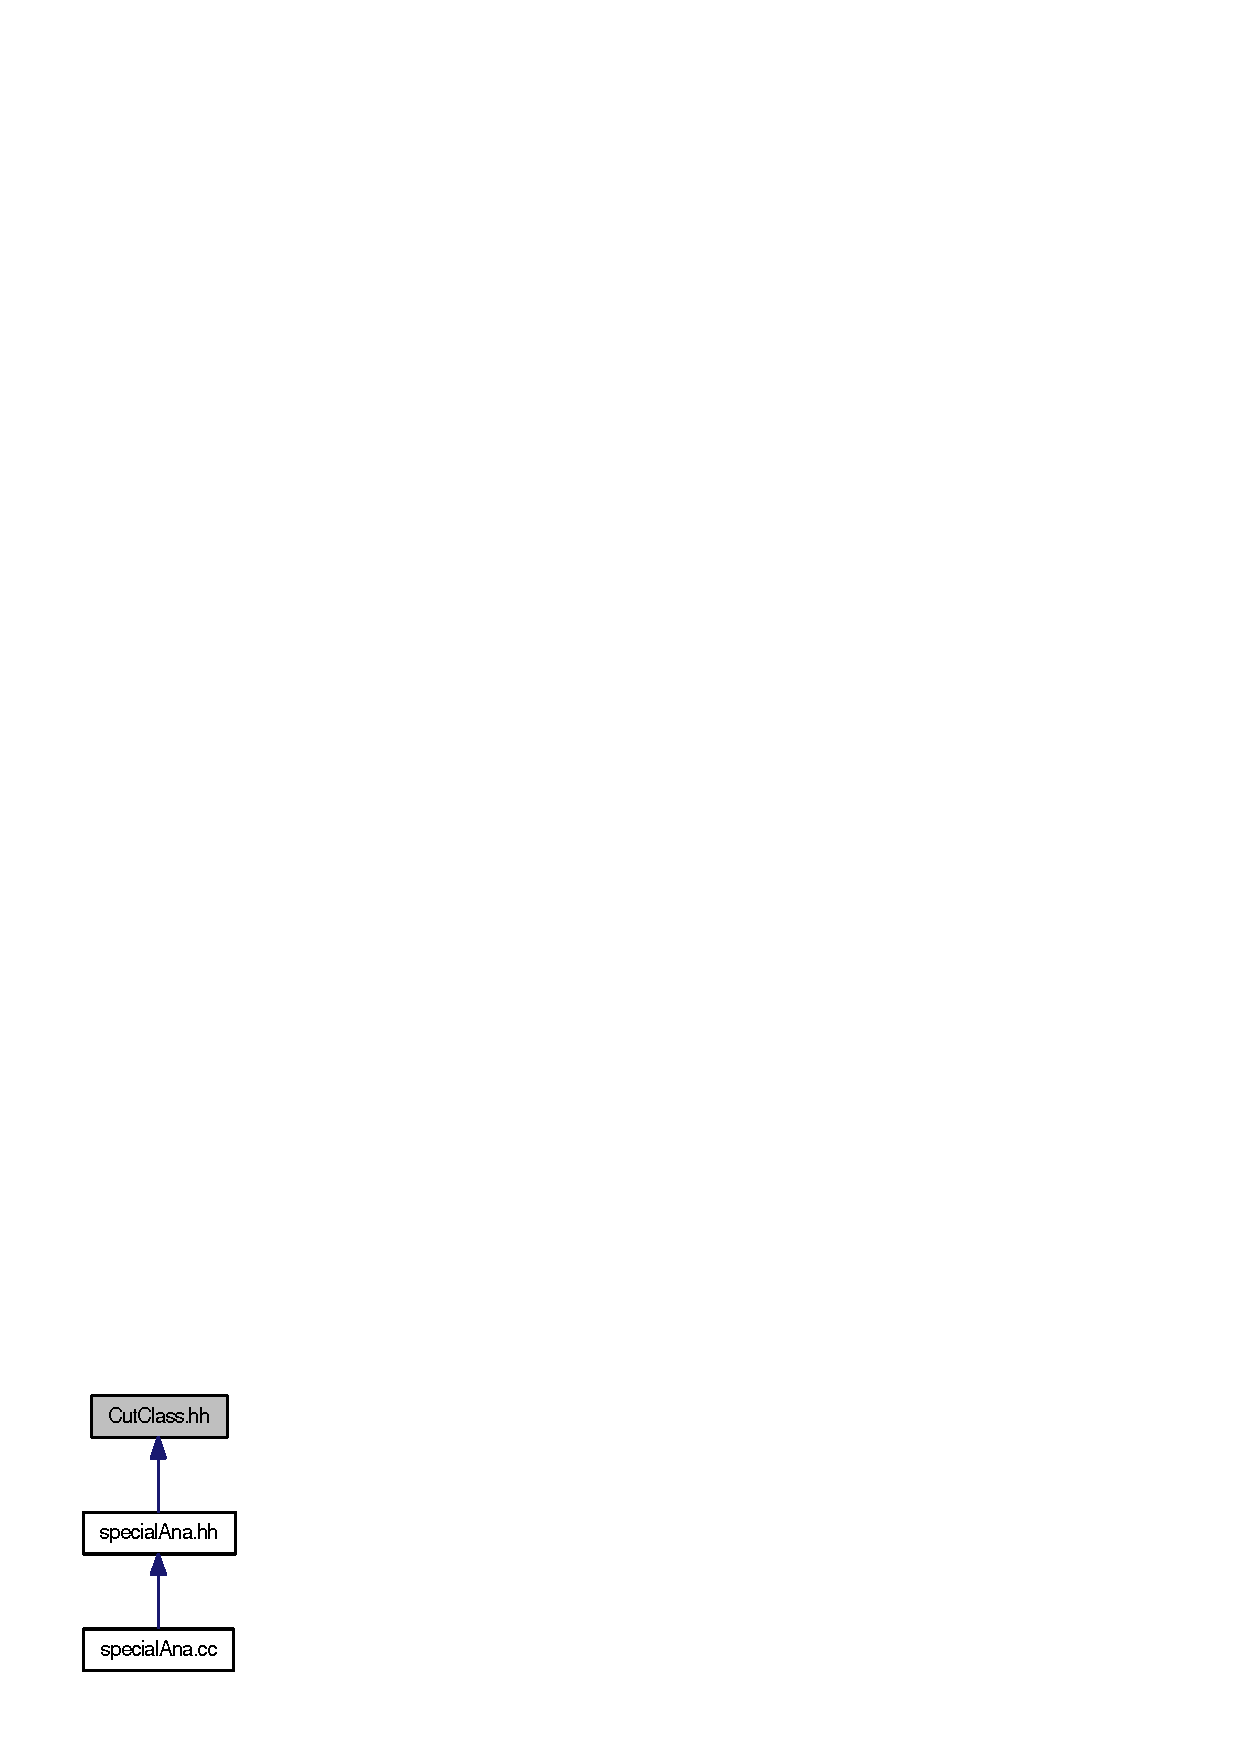
\includegraphics[width=116pt]{CutClass_8hh__dep__incl}
\end{center}
\end{figure}
\subsection*{Classes}
\begin{DoxyCompactItemize}
\item 
class \hyperlink{classCuts}{Cuts}
\end{DoxyCompactItemize}

\section{hooks/githookcontroller.py File Reference}
\label{githookcontroller_8py}\index{hooks/githookcontroller.\-py@{hooks/githookcontroller.\-py}}
\subsection*{Classes}
\begin{DoxyCompactItemize}
\item 
class \hyperlink{classgithookcontroller_1_1GitHookController}{githookcontroller.\-Git\-Hook\-Controller}
\end{DoxyCompactItemize}
\subsection*{Namespaces}
\begin{DoxyCompactItemize}
\item 
\hyperlink{namespacegithookcontroller}{githookcontroller}
\end{DoxyCompactItemize}
\subsection*{Functions}
\begin{DoxyCompactItemize}
\item 
def \hyperlink{namespacegithookcontroller_a5c0a2facfdd7509f64df2aa6aefecf17}{githookcontroller.\-main}
\end{DoxyCompactItemize}
\subsection*{Variables}
\begin{DoxyCompactItemize}
\item 
tuple \hyperlink{namespacegithookcontroller_a3bbdf7a562461bd3baca4ef635d6dd50}{githookcontroller.\-log} = logging.\-get\-Logger( 'githookcontroller' )
\item 
tuple \hyperlink{namespacegithookcontroller_a13f0aa9843a2a5b05ba2e12f5ed3c903}{githookcontroller.\-ch} = logging.\-Stream\-Handler( sys.\-stdout )
\item 
tuple \hyperlink{namespacegithookcontroller_a8672f684f117c8c4733546a0bc9e9616}{githookcontroller.\-formatter} = logging.\-Formatter( '\%(levelname)s (\%(name)s)\-: \%(message)s' )
\item 
tuple \hyperlink{namespacegithookcontroller_ae617d8e0c886ed4e082bd11f1f33bd0d}{githookcontroller.\-Push}
\item 
tuple \hyperlink{namespacegithookcontroller_af0d83e4b5f26b63a7ee452f3eb566ef4}{githookcontroller.\-Commit}
\end{DoxyCompactItemize}

\section{hooks/post-\/commit.py File Reference}
\label{post-commit_8py}\index{hooks/post-\/commit.\-py@{hooks/post-\/commit.\-py}}
\subsection*{Namespaces}
\begin{DoxyCompactItemize}
\item 
\hyperlink{namespacepost-commit}{post-\/commit}
\end{DoxyCompactItemize}

\section{hooks/pre-\/commit.py File Reference}
\label{pre-commit_8py}\index{hooks/pre-\/commit.\-py@{hooks/pre-\/commit.\-py}}
\subsection*{Namespaces}
\begin{DoxyCompactItemize}
\item 
\hyperlink{namespacepre-commit}{pre-\/commit}
\end{DoxyCompactItemize}
\subsection*{Variables}
\begin{DoxyCompactItemize}
\item 
tuple \hyperlink{namespacepre-commit_a95f05a041aa51857ded4a498e766b83d}{pre-\/commit.\-git\-Controller} = Git\-Hook\-Controller()
\item 
tuple \hyperlink{namespacepre-commit_a1c824fbe54d00a54423cb4955f97dcf5}{pre-\/commit.\-changed} = git\-Controller.\-parse\-\_\-pre\-\_\-commit()
\end{DoxyCompactItemize}

\section{hooks/pre-\/push.py File Reference}
\label{pre-push_8py}\index{hooks/pre-\/push.\-py@{hooks/pre-\/push.\-py}}
\subsection*{Namespaces}
\begin{DoxyCompactItemize}
\item 
\hyperlink{namespacepre-push}{pre-\/push}
\end{DoxyCompactItemize}
\subsection*{Variables}
\begin{DoxyCompactItemize}
\item 
tuple \hyperlink{namespacepre-push_a8c127aba641727d65b14a0f4aad44a1c}{pre-\/push.\-git\-Controller} = Git\-Hook\-Controller()
\item 
tuple \hyperlink{namespacepre-push_a71bb0fe33ffeefadee67d3dbbe085080}{pre-\/push.\-push} = git\-Controller.\-parse\-\_\-pre\-\_\-push()
\item 
list \hyperlink{namespacepre-push_a78ac8288356df9910db91d02884f211c}{pre-\/push.\-branchnames} = \mbox{[}commit.\-local\-\_\-branch for commit in push.\-commits\mbox{]}
\end{DoxyCompactItemize}

\section{hooks/\-R\-E\-A\-D\-M\-E.md File Reference}
\label{README_8md}\index{hooks/\-R\-E\-A\-D\-M\-E.\-md@{hooks/\-R\-E\-A\-D\-M\-E.\-md}}

\section{special\-Ana.\-cc File Reference}
\label{specialAna_8cc}\index{special\-Ana.\-cc@{special\-Ana.\-cc}}
{\ttfamily \#include \char`\"{}special\-Ana.\-hh\char`\"{}}\\*
{\ttfamily \#include \char`\"{}Hist\-Class.\-hh\char`\"{}}\\*
{\ttfamily \#include \char`\"{}Tools/\-Tools.\-hh\char`\"{}}\\*
{\ttfamily \#include \char`\"{}boost/format.\-hpp\char`\"{}}\\*
Include dependency graph for special\-Ana.\-cc\-:\nopagebreak
\begin{figure}[H]
\begin{center}
\leavevmode
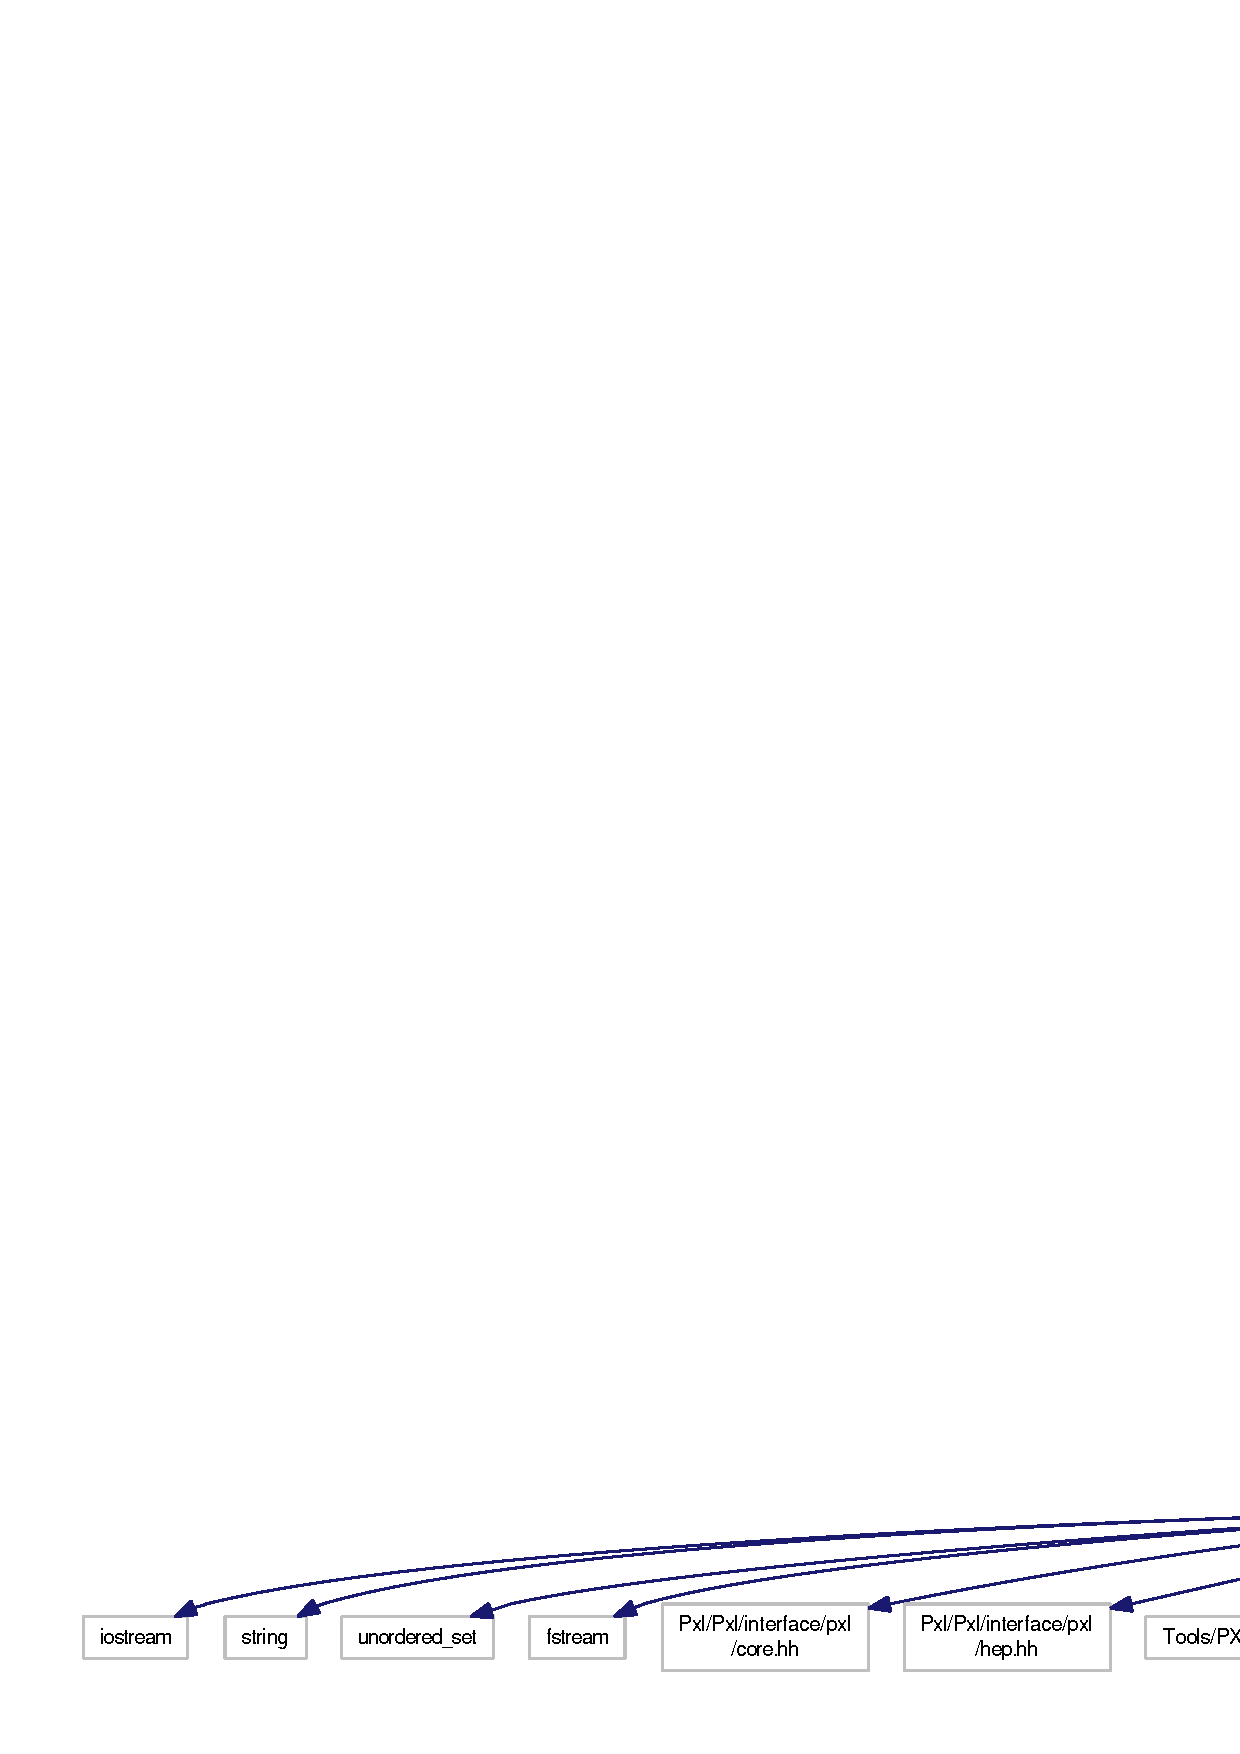
\includegraphics[width=350pt]{specialAna_8cc__incl}
\end{center}
\end{figure}
\subsection*{Functions}
\begin{DoxyCompactItemize}
\item 
\hyperlink{specialAna_8cc_ae54ac397f91803ea463afc9020684e8c}{m\-\_\-data\-Period} (cfg.\-Get\-Item$<$ string $>$(\char`\"{}General.\-Data\-Period\char`\"{}))
\item 
\hyperlink{specialAna_8cc_af0187129768123d4e14e4c2c6319a11a}{m\-\_\-channel} (cfg.\-Get\-Item$<$ string $>$(\char`\"{}R\-P\-V.\-channel\char`\"{}))
\item 
\hyperlink{specialAna_8cc_a573686cdd24430f2c33f7d1c990c8732}{config\-\_\-} (cfg)
\end{DoxyCompactItemize}


\subsection{Function Documentation}
\index{special\-Ana.\-cc@{special\-Ana.\-cc}!config\-\_\-@{config\-\_\-}}
\index{config\-\_\-@{config\-\_\-}!specialAna.cc@{special\-Ana.\-cc}}
\subsubsection[{config\-\_\-}]{\setlength{\rightskip}{0pt plus 5cm}config\-\_\- (
\begin{DoxyParamCaption}
\item[{cfg}]{}
\end{DoxyParamCaption}
)}\label{specialAna_8cc_a573686cdd24430f2c33f7d1c990c8732}


 Init for the e-\/mu channel 

 Init for the e-\/tau\-\_\-h channel 

 Init for the mu-\/tau\-\_\-h channel 

 Init for the e-\/tau\-\_\-e channel 

 Init for the e-\/tau\-\_\-mu channel 

 Init for the mu-\/tau\-\_\-e channel 

 Init for the mu-\/tau\-\_\-mu channel 

Definition at line 21 of file special\-Ana.\-cc.



References m\-\_\-channel(), and m\-\_\-data\-Period().

\index{special\-Ana.\-cc@{special\-Ana.\-cc}!m\-\_\-channel@{m\-\_\-channel}}
\index{m\-\_\-channel@{m\-\_\-channel}!specialAna.cc@{special\-Ana.\-cc}}
\subsubsection[{m\-\_\-channel}]{\setlength{\rightskip}{0pt plus 5cm}m\-\_\-channel (
\begin{DoxyParamCaption}
\item[{cfg.\-Get\-Item$<$ string $>$}]{\char`\"{}\-R\-P\-V.\-channel\char`\"{}}
\end{DoxyParamCaption}
)}\label{specialAna_8cc_af0187129768123d4e14e4c2c6319a11a}


Referenced by config\-\_\-().

\index{special\-Ana.\-cc@{special\-Ana.\-cc}!m\-\_\-data\-Period@{m\-\_\-data\-Period}}
\index{m\-\_\-data\-Period@{m\-\_\-data\-Period}!specialAna.cc@{special\-Ana.\-cc}}
\subsubsection[{m\-\_\-data\-Period}]{\setlength{\rightskip}{0pt plus 5cm}m\-\_\-data\-Period (
\begin{DoxyParamCaption}
\item[{cfg.\-Get\-Item$<$ string $>$}]{\char`\"{}\-General.\-Data\-Period\char`\"{}}
\end{DoxyParamCaption}
)}\label{specialAna_8cc_ae54ac397f91803ea463afc9020684e8c}


Referenced by config\-\_\-().


\section{special\-Ana.\-hh File Reference}
\label{specialAna_8hh}\index{special\-Ana.\-hh@{special\-Ana.\-hh}}
{\ttfamily \#include $<$iostream$>$}\\*
{\ttfamily \#include $<$string$>$}\\*
{\ttfamily \#include $<$unordered\-\_\-set$>$}\\*
{\ttfamily \#include $<$fstream$>$}\\*
{\ttfamily \#include \char`\"{}Pxl/\-Pxl/interface/pxl/core.\-hh\char`\"{}}\\*
{\ttfamily \#include \char`\"{}Pxl/\-Pxl/interface/pxl/hep.\-hh\char`\"{}}\\*
{\ttfamily \#include \char`\"{}Tools/\-P\-X\-L/\-Sort.\-hh\char`\"{}}\\*
{\ttfamily \#include \char`\"{}Tools/\-M\-Config.\-hh\char`\"{}}\\*
{\ttfamily \#include \char`\"{}T\-H1\-F.\-h\char`\"{}}\\*
{\ttfamily \#include \char`\"{}T\-H2\-F.\-h\char`\"{}}\\*
{\ttfamily \#include \char`\"{}T\-String.\-h\char`\"{}}\\*
{\ttfamily \#include \char`\"{}T\-Lorentz\-Vector.\-h\char`\"{}}\\*
{\ttfamily \#include \char`\"{}T\-Efficiency.\-h\char`\"{}}\\*
{\ttfamily \#include $<$T\-File.\-h$>$}\\*
{\ttfamily \#include \char`\"{}Main/\-Systematics.\-hh\char`\"{}}\\*
{\ttfamily \#include \char`\"{}Cut\-Class.\-hh\char`\"{}}\\*
Include dependency graph for special\-Ana.\-hh\-:\nopagebreak
\begin{figure}[H]
\begin{center}
\leavevmode
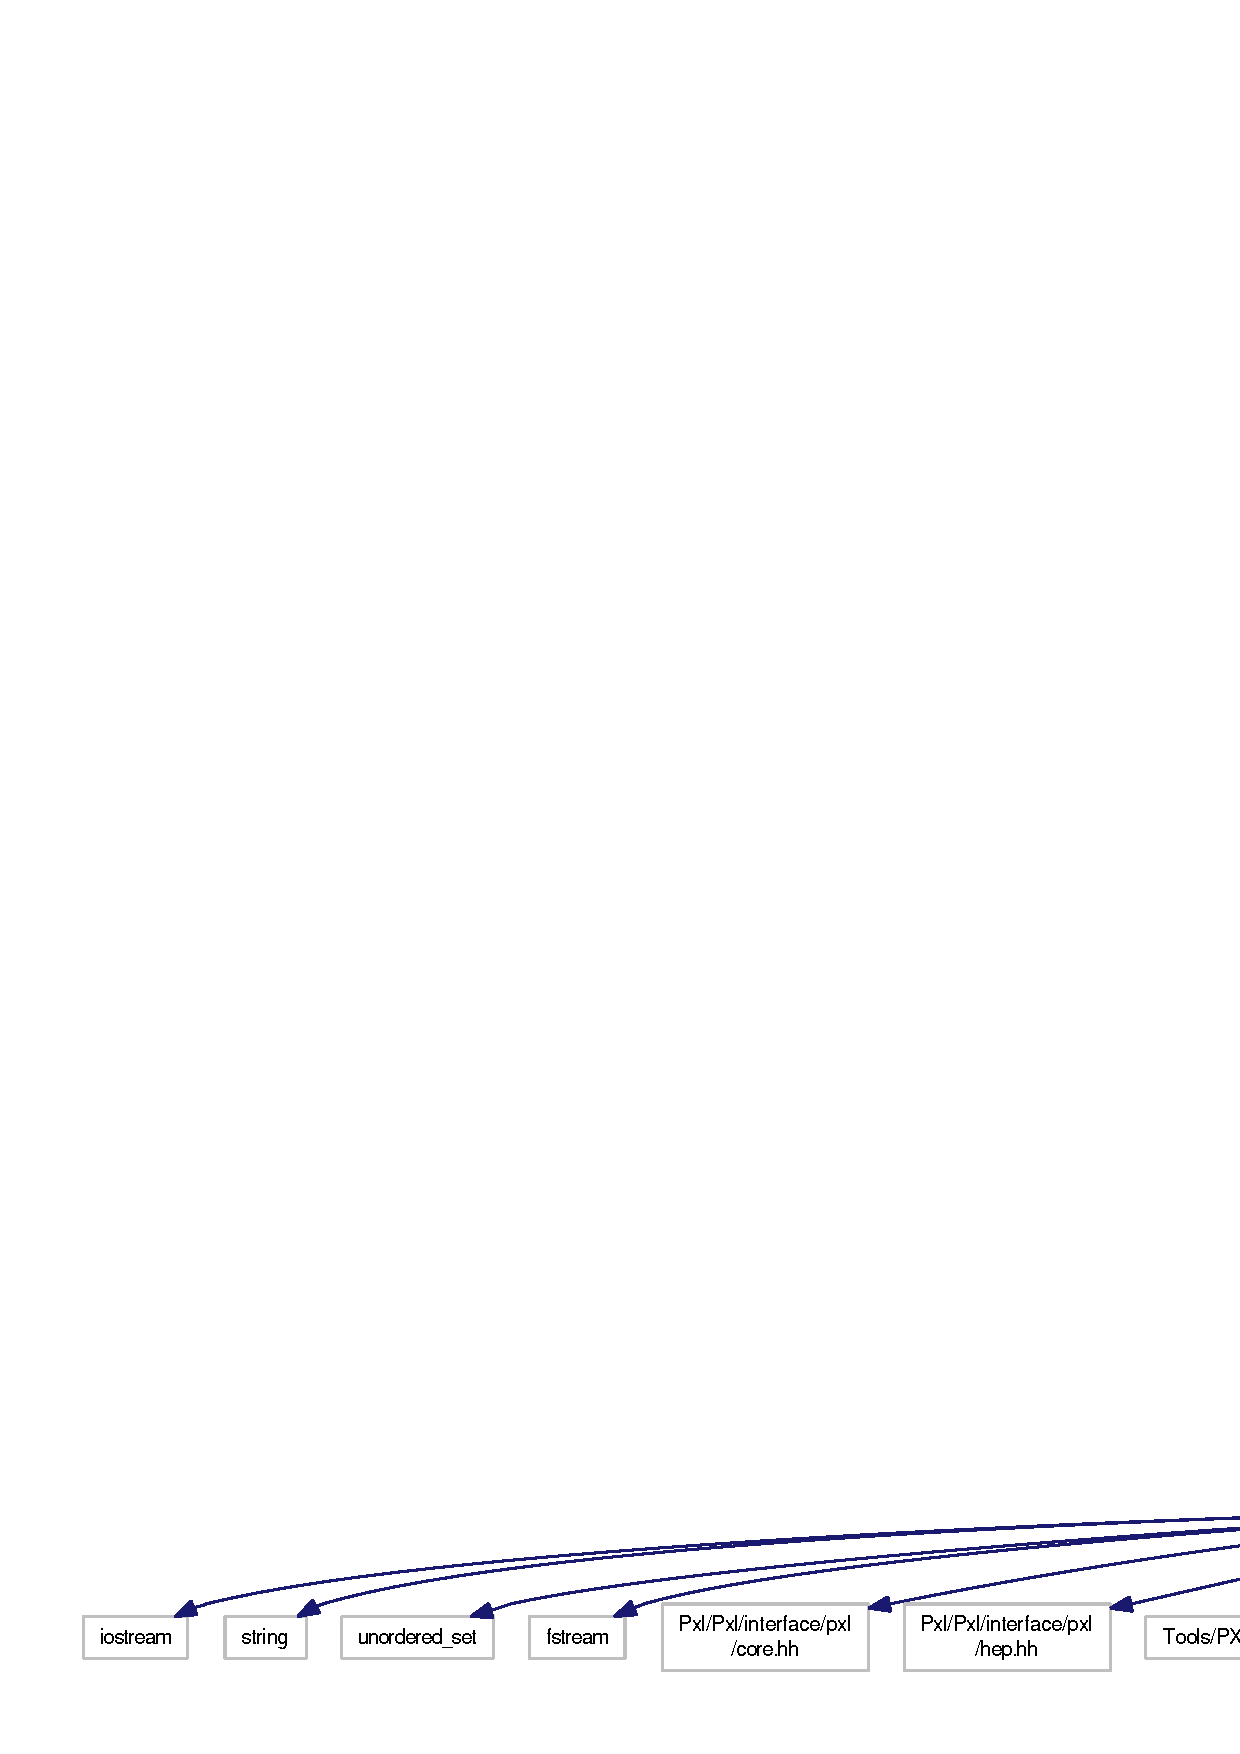
\includegraphics[width=350pt]{specialAna_8hh__incl}
\end{center}
\end{figure}
This graph shows which files directly or indirectly include this file\-:\nopagebreak
\begin{figure}[H]
\begin{center}
\leavevmode
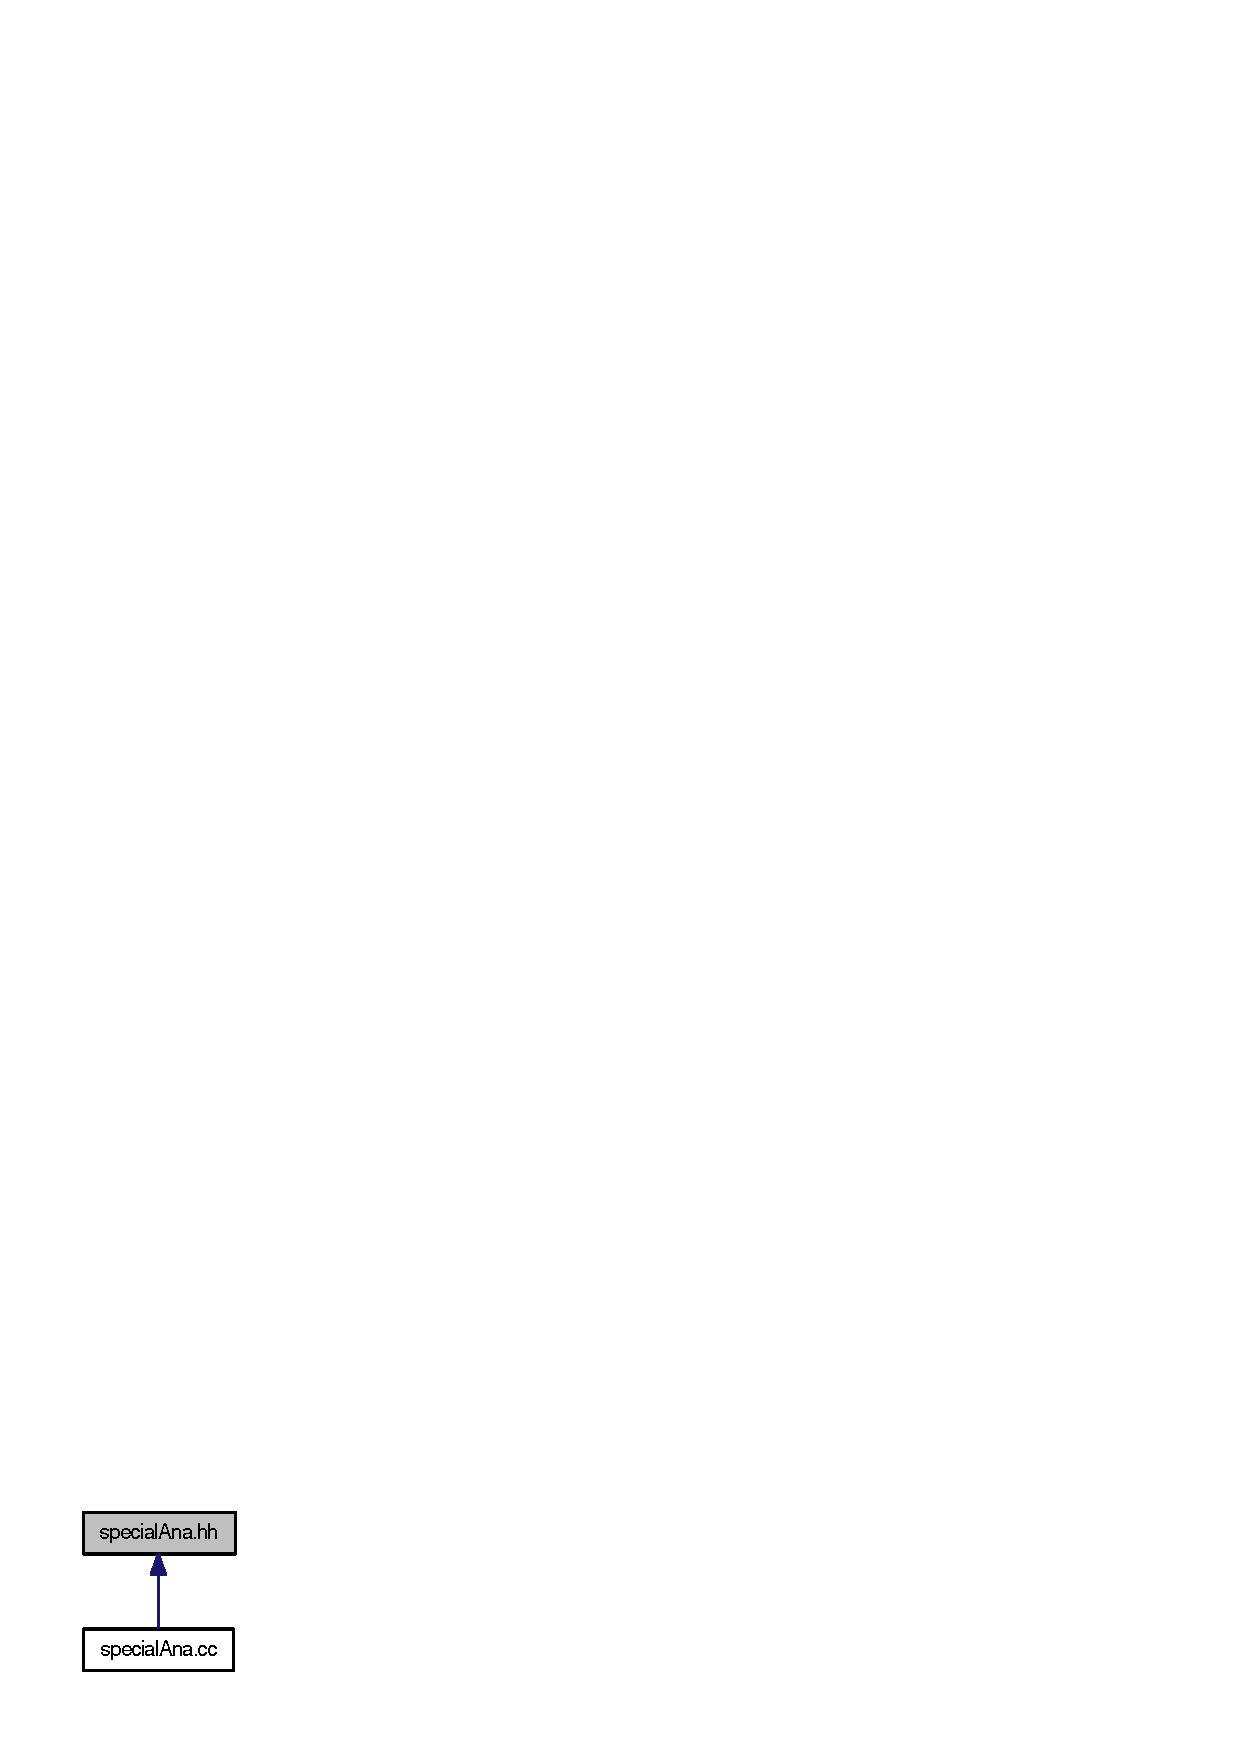
\includegraphics[width=116pt]{specialAna_8hh__dep__incl}
\end{center}
\end{figure}
\subsection*{Classes}
\begin{DoxyCompactItemize}
\item 
class \hyperlink{classspecialAna}{special\-Ana}
\end{DoxyCompactItemize}

%--- End generated contents ---

% Index
\newpage
\phantomsection
\addcontentsline{toc}{part}{Index}
\printindex

\end{document}
